% Options for packages loaded elsewhere
\PassOptionsToPackage{unicode}{hyperref}
\PassOptionsToPackage{hyphens}{url}
%
\documentclass[
]{book}
\usepackage{amsmath,amssymb}
\usepackage{lmodern}
\usepackage{iftex}
\ifPDFTeX
  \usepackage[T1]{fontenc}
  \usepackage[utf8]{inputenc}
  \usepackage{textcomp} % provide euro and other symbols
\else % if luatex or xetex
  \usepackage{unicode-math}
  \defaultfontfeatures{Scale=MatchLowercase}
  \defaultfontfeatures[\rmfamily]{Ligatures=TeX,Scale=1}
\fi
% Use upquote if available, for straight quotes in verbatim environments
\IfFileExists{upquote.sty}{\usepackage{upquote}}{}
\IfFileExists{microtype.sty}{% use microtype if available
  \usepackage[]{microtype}
  \UseMicrotypeSet[protrusion]{basicmath} % disable protrusion for tt fonts
}{}
\makeatletter
\@ifundefined{KOMAClassName}{% if non-KOMA class
  \IfFileExists{parskip.sty}{%
    \usepackage{parskip}
  }{% else
    \setlength{\parindent}{0pt}
    \setlength{\parskip}{6pt plus 2pt minus 1pt}}
}{% if KOMA class
  \KOMAoptions{parskip=half}}
\makeatother
\usepackage{xcolor}
\IfFileExists{xurl.sty}{\usepackage{xurl}}{} % add URL line breaks if available
\IfFileExists{bookmark.sty}{\usepackage{bookmark}}{\usepackage{hyperref}}
\hypersetup{
  pdftitle={My portfolio},
  pdfauthor={Claudia van der Zijden},
  hidelinks,
  pdfcreator={LaTeX via pandoc}}
\urlstyle{same} % disable monospaced font for URLs
\usepackage{color}
\usepackage{fancyvrb}
\newcommand{\VerbBar}{|}
\newcommand{\VERB}{\Verb[commandchars=\\\{\}]}
\DefineVerbatimEnvironment{Highlighting}{Verbatim}{commandchars=\\\{\}}
% Add ',fontsize=\small' for more characters per line
\usepackage{framed}
\definecolor{shadecolor}{RGB}{248,248,248}
\newenvironment{Shaded}{\begin{snugshade}}{\end{snugshade}}
\newcommand{\AlertTok}[1]{\textcolor[rgb]{0.94,0.16,0.16}{#1}}
\newcommand{\AnnotationTok}[1]{\textcolor[rgb]{0.56,0.35,0.01}{\textbf{\textit{#1}}}}
\newcommand{\AttributeTok}[1]{\textcolor[rgb]{0.77,0.63,0.00}{#1}}
\newcommand{\BaseNTok}[1]{\textcolor[rgb]{0.00,0.00,0.81}{#1}}
\newcommand{\BuiltInTok}[1]{#1}
\newcommand{\CharTok}[1]{\textcolor[rgb]{0.31,0.60,0.02}{#1}}
\newcommand{\CommentTok}[1]{\textcolor[rgb]{0.56,0.35,0.01}{\textit{#1}}}
\newcommand{\CommentVarTok}[1]{\textcolor[rgb]{0.56,0.35,0.01}{\textbf{\textit{#1}}}}
\newcommand{\ConstantTok}[1]{\textcolor[rgb]{0.00,0.00,0.00}{#1}}
\newcommand{\ControlFlowTok}[1]{\textcolor[rgb]{0.13,0.29,0.53}{\textbf{#1}}}
\newcommand{\DataTypeTok}[1]{\textcolor[rgb]{0.13,0.29,0.53}{#1}}
\newcommand{\DecValTok}[1]{\textcolor[rgb]{0.00,0.00,0.81}{#1}}
\newcommand{\DocumentationTok}[1]{\textcolor[rgb]{0.56,0.35,0.01}{\textbf{\textit{#1}}}}
\newcommand{\ErrorTok}[1]{\textcolor[rgb]{0.64,0.00,0.00}{\textbf{#1}}}
\newcommand{\ExtensionTok}[1]{#1}
\newcommand{\FloatTok}[1]{\textcolor[rgb]{0.00,0.00,0.81}{#1}}
\newcommand{\FunctionTok}[1]{\textcolor[rgb]{0.00,0.00,0.00}{#1}}
\newcommand{\ImportTok}[1]{#1}
\newcommand{\InformationTok}[1]{\textcolor[rgb]{0.56,0.35,0.01}{\textbf{\textit{#1}}}}
\newcommand{\KeywordTok}[1]{\textcolor[rgb]{0.13,0.29,0.53}{\textbf{#1}}}
\newcommand{\NormalTok}[1]{#1}
\newcommand{\OperatorTok}[1]{\textcolor[rgb]{0.81,0.36,0.00}{\textbf{#1}}}
\newcommand{\OtherTok}[1]{\textcolor[rgb]{0.56,0.35,0.01}{#1}}
\newcommand{\PreprocessorTok}[1]{\textcolor[rgb]{0.56,0.35,0.01}{\textit{#1}}}
\newcommand{\RegionMarkerTok}[1]{#1}
\newcommand{\SpecialCharTok}[1]{\textcolor[rgb]{0.00,0.00,0.00}{#1}}
\newcommand{\SpecialStringTok}[1]{\textcolor[rgb]{0.31,0.60,0.02}{#1}}
\newcommand{\StringTok}[1]{\textcolor[rgb]{0.31,0.60,0.02}{#1}}
\newcommand{\VariableTok}[1]{\textcolor[rgb]{0.00,0.00,0.00}{#1}}
\newcommand{\VerbatimStringTok}[1]{\textcolor[rgb]{0.31,0.60,0.02}{#1}}
\newcommand{\WarningTok}[1]{\textcolor[rgb]{0.56,0.35,0.01}{\textbf{\textit{#1}}}}
\usepackage{longtable,booktabs,array}
\usepackage{calc} % for calculating minipage widths
% Correct order of tables after \paragraph or \subparagraph
\usepackage{etoolbox}
\makeatletter
\patchcmd\longtable{\par}{\if@noskipsec\mbox{}\fi\par}{}{}
\makeatother
% Allow footnotes in longtable head/foot
\IfFileExists{footnotehyper.sty}{\usepackage{footnotehyper}}{\usepackage{footnote}}
\makesavenoteenv{longtable}
\usepackage{graphicx}
\makeatletter
\def\maxwidth{\ifdim\Gin@nat@width>\linewidth\linewidth\else\Gin@nat@width\fi}
\def\maxheight{\ifdim\Gin@nat@height>\textheight\textheight\else\Gin@nat@height\fi}
\makeatother
% Scale images if necessary, so that they will not overflow the page
% margins by default, and it is still possible to overwrite the defaults
% using explicit options in \includegraphics[width, height, ...]{}
\setkeys{Gin}{width=\maxwidth,height=\maxheight,keepaspectratio}
% Set default figure placement to htbp
\makeatletter
\def\fps@figure{htbp}
\makeatother
\setlength{\emergencystretch}{3em} % prevent overfull lines
\providecommand{\tightlist}{%
  \setlength{\itemsep}{0pt}\setlength{\parskip}{0pt}}
\setcounter{secnumdepth}{5}
\usepackage{booktabs}
\ifLuaTeX
  \usepackage{selnolig}  % disable illegal ligatures
\fi
\usepackage[]{natbib}
\bibliographystyle{apalike}

\title{My portfolio}
\author{Claudia van der Zijden}
\date{2021-06-20}

\begin{document}
\maketitle

{
\setcounter{tocdepth}{1}
\tableofcontents
}
\hypertarget{introduction}{%
\chapter{Introduction}\label{introduction}}

Welkom to my portfolio!

In my portfolio I try to give an impression of my programming skills. This is mainly in r but I also have some experience with bash.

This portfolio contains a number of chapters with assignments that I have made, it also contains my resume. The last chapter called machine learning is about a tutorial assignment in which I tried to learn more about machine learning.

I hope this portfolio will give you a good idea of my skills.

For further questions you can always email \href{mailto:claudiavanderzijden@hotmail.nl}{\nolinkurl{claudiavanderzijden@hotmail.nl}}

\hypertarget{reproducible-research}{%
\chapter{Reproducible research}\label{reproducible-research}}

C. elegans plate experiment

\emph{The data for this exercise was kindly supplied by J. Louter (INT/ILC) and was derived from an experiment in which adult C.elegans nematodes were exposed to varying concentrations of different compounds. The variables RawData (the outcome - number of offspring counted as an integer value, after incubation time), compName (the generic name of the compound/chemical), the compConcentration (the concentration of the compound), and the expType are the most important variables in this dataset.}

\emph{A typical analysis with this data would be to run a dose-response analysis using a log-logistic model with estimates for the maximal, the minimal, the IC50 concentration and the slope at IC50. We will not go into the details but a good package to run such computations and create graphs in R is the \{drc\} package. See: and:. In the exercise below we will create some visualizations using \{ggplot2\}.}

Before we start, we will inspect the dataset. We do this by opening it in Excel. When you look at this dataset, a few things stand out. Among other things, there are many tabs with very large tables without an explanation. This makes it difficult for outsiders to use this data.

Then we will load the data into rstudio.

\begin{Shaded}
\begin{Highlighting}[]
\FunctionTok{library}\NormalTok{(tidyverse)}
\end{Highlighting}
\end{Shaded}

\begin{verbatim}
## -- Attaching packages --------------------------------------- tidyverse 1.3.1 --
\end{verbatim}

\begin{verbatim}
## v ggplot2 3.3.3     v purrr   0.3.4
## v tibble  3.1.2     v dplyr   1.0.6
## v tidyr   1.1.3     v stringr 1.4.0
## v readr   1.4.0     v forcats 0.5.1
\end{verbatim}

\begin{verbatim}
## -- Conflicts ------------------------------------------ tidyverse_conflicts() --
## x dplyr::filter() masks stats::filter()
## x dplyr::lag()    masks stats::lag()
\end{verbatim}

\begin{Shaded}
\begin{Highlighting}[]
\FunctionTok{library}\NormalTok{(readxl)}
\NormalTok{ce\_liq\_flow\_062 }\OtherTok{\textless{}{-}} \FunctionTok{read\_excel}\NormalTok{(}\StringTok{"data/CE.LIQ.FLOW.062\_Tidydata.xlsx"}\NormalTok{, }\AttributeTok{sheet =} \DecValTok{1}\NormalTok{)}
\end{Highlighting}
\end{Shaded}

Now we can look at the data types. we will do this for the columns rawData, compName and compConcentration.

\begin{Shaded}
\begin{Highlighting}[]
\FunctionTok{typeof}\NormalTok{(ce\_liq\_flow\_062}\SpecialCharTok{$}\NormalTok{RawData)}
\end{Highlighting}
\end{Shaded}

\begin{verbatim}
## [1] "double"
\end{verbatim}

\begin{Shaded}
\begin{Highlighting}[]
\FunctionTok{typeof}\NormalTok{(ce\_liq\_flow\_062}\SpecialCharTok{$}\NormalTok{compName)}
\end{Highlighting}
\end{Shaded}

\begin{verbatim}
## [1] "character"
\end{verbatim}

\begin{Shaded}
\begin{Highlighting}[]
\FunctionTok{typeof}\NormalTok{(ce\_liq\_flow\_062}\SpecialCharTok{$}\NormalTok{compConcentration)}
\end{Highlighting}
\end{Shaded}

\begin{verbatim}
## [1] "character"
\end{verbatim}

You would expect comConcentration to be numeric but as you can see this is character.

Now we are going to make a scatter plot of the data. We put compconcentration on the x-axis and DataRaw on the y-axis. We give a different color to the levels of compname and a different shape to the levels of expType. In addition, we ensure that the numbers below the x-axis are rotated 45 degrees so that we can read those.

\begin{Shaded}
\begin{Highlighting}[]
\FunctionTok{ggplot}\NormalTok{(}\AttributeTok{data =}\NormalTok{ ce\_liq\_flow\_062, }\FunctionTok{aes}\NormalTok{(}\AttributeTok{x =}\NormalTok{ compConcentration, }\AttributeTok{y =}\NormalTok{ RawData)) }\SpecialCharTok{+}
  \FunctionTok{geom\_point}\NormalTok{(}\FunctionTok{aes}\NormalTok{(}\AttributeTok{colour =}\NormalTok{ compName, }\AttributeTok{shape =}\NormalTok{ expType)) }\SpecialCharTok{+}
   \FunctionTok{scale\_x\_discrete}\NormalTok{(}\AttributeTok{guide =} \FunctionTok{guide\_axis}\NormalTok{(}\AttributeTok{angle =} \DecValTok{45}\NormalTok{)) }\SpecialCharTok{+}
  \FunctionTok{labs}\NormalTok{(}\AttributeTok{title =} \StringTok{"compConcentration is double"}\NormalTok{)}
\end{Highlighting}
\end{Shaded}

\begin{verbatim}
## Warning: Removed 5 rows containing missing values (geom_point).
\end{verbatim}

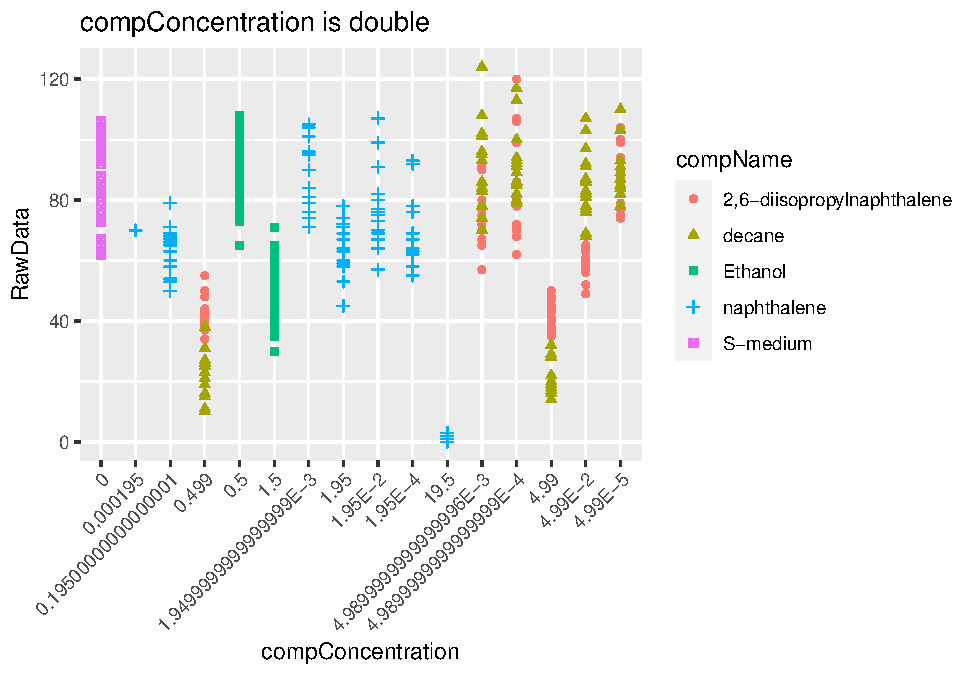
\includegraphics{Nexttry_files/figure-latex/1.1D-1.pdf}

If we now look at this plot, you can see that the scale of the x-axis is not linearly distributed. This is probably due to the data type of comcondition. So we're going to change it to numeric. Then we will plot the data again. We now use a log10 transformation to improve the distribution of the x-axis. We also use jitter to avoid overlapping data points.

\begin{Shaded}
\begin{Highlighting}[]
\NormalTok{ce\_liq\_flow\_062}\SpecialCharTok{$}\NormalTok{compConcentration }\OtherTok{\textless{}{-}} \FunctionTok{as.numeric}\NormalTok{(}\FunctionTok{as.character}\NormalTok{(ce\_liq\_flow\_062}\SpecialCharTok{$}\NormalTok{compConcentration))}
\end{Highlighting}
\end{Shaded}

\begin{verbatim}
## Warning: NAs introduced by coercion
\end{verbatim}

\begin{Shaded}
\begin{Highlighting}[]
\FunctionTok{typeof}\NormalTok{(ce\_liq\_flow\_062}\SpecialCharTok{$}\NormalTok{compConcentration)}
\end{Highlighting}
\end{Shaded}

\begin{verbatim}
## [1] "double"
\end{verbatim}

\begin{Shaded}
\begin{Highlighting}[]
\NormalTok{log10\_scatter }\OtherTok{\textless{}{-}}\FunctionTok{ggplot}\NormalTok{(}\AttributeTok{data =}\NormalTok{ ce\_liq\_flow\_062, }\FunctionTok{aes}\NormalTok{(}\AttributeTok{x =}\NormalTok{ compConcentration, }\AttributeTok{y =}\NormalTok{ RawData)) }\SpecialCharTok{+}
  \FunctionTok{geom\_point}\NormalTok{(}\AttributeTok{position=}\FunctionTok{position\_jitter}\NormalTok{(}\AttributeTok{width=}\NormalTok{.}\DecValTok{1}\NormalTok{,}\AttributeTok{height=}\DecValTok{0}\NormalTok{),}\FunctionTok{aes}\NormalTok{(}\AttributeTok{colour =}\NormalTok{ compName, }\AttributeTok{shape =}\NormalTok{ compName)) }\SpecialCharTok{+}
   \FunctionTok{scale\_x\_discrete}\NormalTok{(}\AttributeTok{guide =} \FunctionTok{guide\_axis}\NormalTok{(}\AttributeTok{angle =} \DecValTok{45}\NormalTok{))}\SpecialCharTok{+}
   \FunctionTok{labs}\NormalTok{(}\AttributeTok{title =} \StringTok{"compConcentration is numeric"}\NormalTok{) }


\NormalTok{log10\_scatter }\SpecialCharTok{+} \FunctionTok{scale\_x\_log10}\NormalTok{()}
\end{Highlighting}
\end{Shaded}

\begin{verbatim}
## Scale for 'x' is already present. Adding another scale for 'x', which will
## replace the existing scale.
\end{verbatim}

\begin{verbatim}
## Warning: Transformation introduced infinite values in continuous x-axis
\end{verbatim}

\begin{verbatim}
## Warning: Removed 6 rows containing missing values (geom_point).
\end{verbatim}

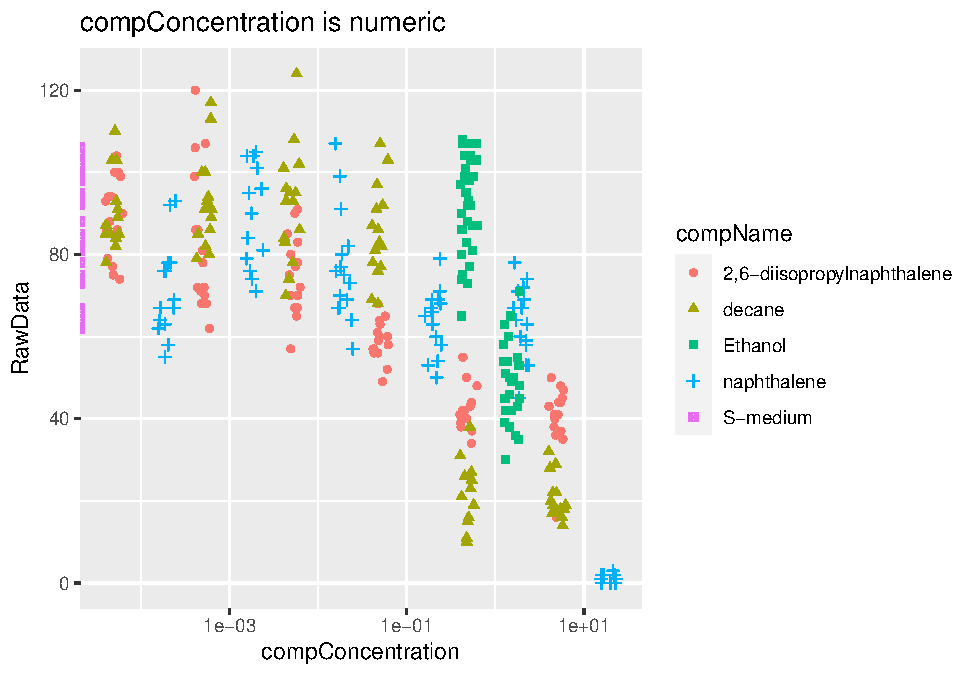
\includegraphics{Nexttry_files/figure-latex/1.1F-1.pdf}

The positive control for this experiments is \textbf{naphthale}. The negative control for this experiment is \textbf{S-medium}.

After reviewing the data, we could proceed with the analysis of the data to find out whether there is indeed an effect of different concentrations on offspring count and whether the different compounds have a different curve. To find out, first check whether the data is normally distributed. This can be done with the shapio-wilk test. This can be used to determine whether a parametric or non-parametric test can be used to see if there is a statistically significant difference between the different groups.

Finaly we normalize the data for the controlNegative in such a way that the mean value for controlNegative is exactly equal to 1 and all other values are expressed as a fraction thereof. Than we rerun the graph with the normalized data.

\#``\{r 1.1J\}
normalize \textless- function(x) \{
return ((x - min(x)) / (max(x) - min(x)))
\}

ce\_liq\_flow\_062\(compVehicle %>% normalize(filter(ce_liq_flow_062
\)compVehicle == ``controlNegative''))

\begin{verbatim}


H.Why would you want to take the step under J?

<!--chapter:end:01-Reproducible_Research.Rmd-->

# Open Peer Review

In this assisgment w arw goning to find a scientific article ourself, using PubMed or another database or repository. We'll use only Open Access articles. When we fond a article we will go over the Transparency Criteria.

This is the link to the article I use
https://www.biorxiv.org/content/10.1101/2020.10.02.322917v2.full

The title of this article is: Leveraging high-throughput screening data and conditional generative adversarial networks to advance predictive toxicology
The authors of this article are: Adrian J. Green, Martin J. Mohlenkamp, Jhuma Das, et al.

## Peer revieuw part 1

__Study Purpose__ : the summary briefly explains what is more important to conduct this research <br/>
__Data Availability Statement__: not present <br/>
__Data Location__: it does describe what the data should look like and there are references to articles that describe how the data was collected. It does not say where you can find the used data. <br/>
__Study Location__: there is no information about where the study was conducted in the material and method section <br/>
__Author Review__: the details of the authors are not easy to obtain, the names of the authors are at the top of the article but further contact details are not on the page itself. <br/>
__Ethics Statement__: the introduction briefly mentions ethics <br/>
__Funding Statement__: nothing is said about funding <br/>
__Code Availability__: no code is shared in the article <br/>

## Open peer review part 2
Next we are going to try to find a article with R code. We do this on the OSF website.
We are going to try to get the code working in our r studio. 

This is the link to the code we will use
https://osf.io/gkcn7/

To make this code work we only have to change the way to load the data, out commend the effect sizes and we have to change the column names so the names are not separated by points. 

You can find the working script in the appendix, chapther 11

It took little effort to get this script working. On a scale of 0 to 5 I would give it a 4

<!--chapter:end:02-Open_peer_review.Rmd-->

# Guerrilla analytics

In this assignment I cleaned up my projects according to the Guerrilla analytics.The result can be seen below onder. 

## Daur2 project
![Claudia](data/Gurilla/Daur2.png){ width=70%}


## Portfolio project
![Claudia](data/Gurilla/portfolio.png){ width=70%}


## Project project
![Claudia](data/Gurilla/project.png){ width=70%}





<!--chapter:end:03-Guerrilla_analytics.Rmd-->

# Curriculum vitae

![Claudia](data/CV/cvfoto.png){ width=100%}

<!--chapter:end:04-Curriculum_vitae.Rmd-->

# Mendaly

In practice, many use has been made of RNA sequencing (RNA-seq) methods. With RNA-seq, the transcriptional activity of cells can be examined. Next-generation sequencing is used for this. This results in transcriptomics datasets, which makes it difficult for many researchers to process this data and to draw conclusions from it. [@Marini2020]. That is why in this project we are working on a way in which researchers without programming knowledge can easily process transcriptome data. The aim is to develop a shiny app where only a GSE/SRA number needs to be entered, after which an analysis is performed automatically. This saves researchers a lot of time. To make this possible, we use salmon and DESeq2 among others. A GSE number can be used to search the SRA database for a dataset in the form of a fastq file. This fastq file can be used in Salmon. Salmon is a package that quantifies the data.[@Patro2017] . When quantifying the data, it is determined how many of the parts of the data correspond to the reference data. Because Salmon takes small pieces of the data for testing, it works much faster and takes much less memory to perform this analysis than other methods. The analyzed data that then comes from the salmon analysis will be further investigated using deseq2. The DESeq2 package provides methods to test for differential expression using negative binomial generalized linear models. [@rnaseq] A sumerised experiment is then made of this data. [@sumexp] A sumerised experiment is a container where data is stored in different dimensions. It contains row data, it contains information about the genes, and the cold data also contains information about the samples. Finally, the sumerised experiment also contains the number of counts. A sumerised experiment will serve as input for the ISEE shiny app. This ISEE app has been specially developed for analyzing transcriptome data [@Lun2018] In this app not only the count data are processed, but also the row data and the cold data are displayed in graphs. This makes the analysis very comprehensive.
In our project we also want to pay attention to a new shiny app. Although the ISEE app is a well-functioning app, there are a number of things that we miss. For example, we think that the app is not clear enough because all graphs are plotted on one page without further additions. In addition, we miss a way in which you can enter the GSE/SRA number. So you still need some programming skills to use this app.
Ultimately, it would be nice if you only had to fill in a dataset and you would then receive a message as soon as the analysis is ready. At the moment this analysis is ready, it would be nice if a ready-made report could be downloaded with the result processing and statistical tests in it.

<!--chapter:end:05-Mendely.Rmd-->

# Relational databases

TIPS

Be aware, the flu and dengue data contains metadata that should be stripped from the data on load.
Think of a way to create valid country names that fit with the gapminder data.
Remember (!) that in the end, this assignment needs to be reported by a .Rmd file for your portfolio. So save what you are doing, save your SQL scripts, make screenshots if you want, and in general design a clear and attractive report in RMarkdown to showcase your SQL/database-skills in your portfolio. You may be sending this to propspective employers in the future! (also, the portfolio is what we as teachers will be grading. But definitely think about the future rather than only about “passing the course”)
Assignment

Load the flu (“./data/flu_data.csv), the dengue (.”/data/dengue_data.csv) and the gapminder ({dslabs} package) into three separate dataframes in R

Check if they are in the right shape. Is the data in the ‘tidy’ format? If not change the format to ‘tidy’

Change the country and date variables of the three tables so that they coincide in terms of data type, class and values

Store the three tables as separate (so six in total) .csv and .rds files.

In Dbeaver create a new PostgreSQL database “workflowsdb”

Using RPostgreSQL, insert the tables into the database.

Inspect the contents of the tables with SQL (in DBeaver) and save the SQL script.

Inspect the contents of the tables with dplyr (in R) and save a RMarkdown showing what you are doing.

Load the gapminder data in R and change the dataframe in such as way that you could join it to dengue and flue.

Save this clean gapminder data in the “workflowsdb” database

Perform some joins (your choice) with SQL (can be done in DBeaver or with dplyr.

Generate a joined table, and export this from the database to R.

Show some descriptive statistics with this table, and at least 3 visualisations using ggplot2.

show all of your actions in this assignment in a Rmd file, perhaps with pictures and provide text explaining and showcasing your skills.

```r
library(tidyverse)
library(dslabs)
gapminder <- as_tibble(gapminder)
flu_data<- read.csv(url("https://raw.githubusercontent.com/ClaudiavdZ/tlsc-dsfb26v-20_workflows/main/data/flu_data.csv"), skip = 11)
flu_data <- as_tibble(flu_data)
dengue_data<- read.csv(url("https://raw.githubusercontent.com/ClaudiavdZ/tlsc-dsfb26v-20_workflows/main/data/dengue_data.csv"), skip = 11)

write.table(dengue_data , file = "dengu_data.csv")
write.table(dengue_data , file = "dengu_data.RDS")
write.table(flu_data , file = "flu_data.csv")
write.table(flu_data , file = "flu_data.RDS")
write.table(gapminder , file = "gapminder.csv")
write.table(gapminder , file = "gapminder.RDS")

library(DBI)
con <- dbConnect(RPostgres::Postgres(), 
                 dbname = "myfirstdb", 
                 host="localhost", 
                 port="5432", 
                 user="postgres", 
                 password="Veroni36") 
dbListTables(con) 
\end{verbatim}

\begin{verbatim}
## [1] "test"        "gapminder"   "flu_data"    "dengue_data"
\end{verbatim}

\begin{Shaded}
\begin{Highlighting}[]
\CommentTok{\#dbWriteTable(con, "dengue\_data", dengue\_data)}
\CommentTok{\#dbWriteTable(con, "flu\_data", flu\_data)}
\CommentTok{\#dbWriteTable(con, "gapminder", gapminder)}

\CommentTok{\# library(janitor)}
\CommentTok{\# gapminder\_usd \textless{}{-} as.data.frame(t(gapminder))}
\CommentTok{\# gapminder\_usd \textless{}{-} gapminder\_usd \%\textgreater{}\% row\_to\_names(row\_number = 1)}


\NormalTok{flu\_usd }\OtherTok{\textless{}{-}} \FunctionTok{gather}\NormalTok{(}
\NormalTok{  flu\_data,}
  \AttributeTok{key =} \StringTok{"country"}\NormalTok{,}
  \AttributeTok{value =} \StringTok{"flu"}\NormalTok{,}
\NormalTok{  Argentina}\SpecialCharTok{:}\NormalTok{Uruguay}
\NormalTok{)}
\CommentTok{\#seperate year from month and day}
\NormalTok{flu\_usd }\OtherTok{\textless{}{-}} \FunctionTok{separate}\NormalTok{(flu\_usd, Date, }\AttributeTok{into =} \FunctionTok{c}\NormalTok{(}\StringTok{"year"}\NormalTok{, }\StringTok{"month"}\NormalTok{, }\StringTok{"day"}\NormalTok{),  }\AttributeTok{sep =} \StringTok{"{-}"}\NormalTok{)}
\CommentTok{\#count sum of flu}
\NormalTok{flu\_usd }\OtherTok{\textless{}{-}} \FunctionTok{aggregate}\NormalTok{(flu\_usd}\SpecialCharTok{$}\NormalTok{flu, }\AttributeTok{by=}\FunctionTok{list}\NormalTok{(}\AttributeTok{year=}\NormalTok{flu\_usd}\SpecialCharTok{$}\NormalTok{year, }\AttributeTok{country=}\NormalTok{flu\_usd}\SpecialCharTok{$}\NormalTok{country), }\AttributeTok{FUN=}\NormalTok{sum)}
\NormalTok{flu\_usd }\OtherTok{\textless{}{-}}\NormalTok{ flu\_usd }\SpecialCharTok{\%\textgreater{}\%} \FunctionTok{rename}\NormalTok{(}\AttributeTok{flu =}\NormalTok{ x)}
\NormalTok{flu\_usd}\SpecialCharTok{$}\NormalTok{year }\OtherTok{\textless{}{-}} \FunctionTok{as.integer}\NormalTok{(flu\_usd}\SpecialCharTok{$}\NormalTok{year)  }

\NormalTok{dengue\_usd }\OtherTok{\textless{}{-}} \FunctionTok{gather}\NormalTok{(}
\NormalTok{  dengue\_data,}
  \AttributeTok{key =} \StringTok{"country"}\NormalTok{,}
  \AttributeTok{value =} \StringTok{"dengue"}\NormalTok{,}
\NormalTok{  Argentina}\SpecialCharTok{:}\NormalTok{Venezuela}
\NormalTok{)}
\NormalTok{dengue\_usd }\OtherTok{\textless{}{-}} \FunctionTok{separate}\NormalTok{(dengue\_usd, Date, }\AttributeTok{into =} \FunctionTok{c}\NormalTok{(}\StringTok{"year"}\NormalTok{, }\StringTok{"month"}\NormalTok{, }\StringTok{"day"}\NormalTok{),  }\AttributeTok{sep =} \StringTok{"{-}"}\NormalTok{)}
\NormalTok{dengue\_usd }\OtherTok{\textless{}{-}} \FunctionTok{aggregate}\NormalTok{(dengue\_usd}\SpecialCharTok{$}\NormalTok{dengue, }\AttributeTok{by=}\FunctionTok{list}\NormalTok{(}\AttributeTok{year=}\NormalTok{dengue\_usd}\SpecialCharTok{$}\NormalTok{year, }\AttributeTok{country=}\NormalTok{dengue\_usd}\SpecialCharTok{$}\NormalTok{country), }\AttributeTok{FUN=}\NormalTok{sum)}
\NormalTok{dengue\_usd }\OtherTok{\textless{}{-}}\NormalTok{ dengue\_usd }\SpecialCharTok{\%\textgreater{}\%} \FunctionTok{rename}\NormalTok{(}\AttributeTok{dengue =}\NormalTok{ x)}
\NormalTok{dengue\_usd}\SpecialCharTok{$}\NormalTok{year }\OtherTok{\textless{}{-}} \FunctionTok{as.integer}\NormalTok{(dengue\_usd}\SpecialCharTok{$}\NormalTok{year)}

\NormalTok{alltogether }\OtherTok{\textless{}{-}} \FunctionTok{left\_join}\NormalTok{(flu\_usd, gapminder, }\AttributeTok{by =} \FunctionTok{c}\NormalTok{(}\StringTok{"country"}\NormalTok{, }\StringTok{"year"}\NormalTok{))}
\NormalTok{alltogether }\OtherTok{\textless{}{-}} \FunctionTok{left\_join}\NormalTok{(alltogether, dengue\_usd , }\AttributeTok{by =} \FunctionTok{c}\NormalTok{(}\StringTok{"country"}\NormalTok{, }\StringTok{"year"}\NormalTok{))}



\CommentTok{\#infant\_mortelity firtelety life expantie door flu and dengue in verschillende jaren in verschillende landen}
\CommentTok{\#en beetje statestiek}
\NormalTok{flu\_plot }\OtherTok{\textless{}{-}} \ControlFlowTok{function}\NormalTok{(dataframe, land)\{}
\NormalTok{  dataframe }\SpecialCharTok{\%\textgreater{}\%} \FunctionTok{filter}\NormalTok{(country }\SpecialCharTok{==}\NormalTok{ land) }\SpecialCharTok{\%\textgreater{}\%} 
    \FunctionTok{ggplot}\NormalTok{(}\FunctionTok{aes}\NormalTok{(}\AttributeTok{x =}\NormalTok{ year, }\AttributeTok{y =}\NormalTok{ flu)) }\SpecialCharTok{+}
  \FunctionTok{geom\_line}\NormalTok{() }\SpecialCharTok{+}
  \FunctionTok{geom\_point}\NormalTok{() }
\NormalTok{  \}}

\FunctionTok{flu\_plot}\NormalTok{(alltogether,}\StringTok{"Netherlands"}\NormalTok{)}
\end{Highlighting}
\end{Shaded}

\begin{verbatim}
## Warning: Removed 2 row(s) containing missing values (geom_path).
\end{verbatim}

\begin{verbatim}
## Warning: Removed 2 rows containing missing values (geom_point).
\end{verbatim}

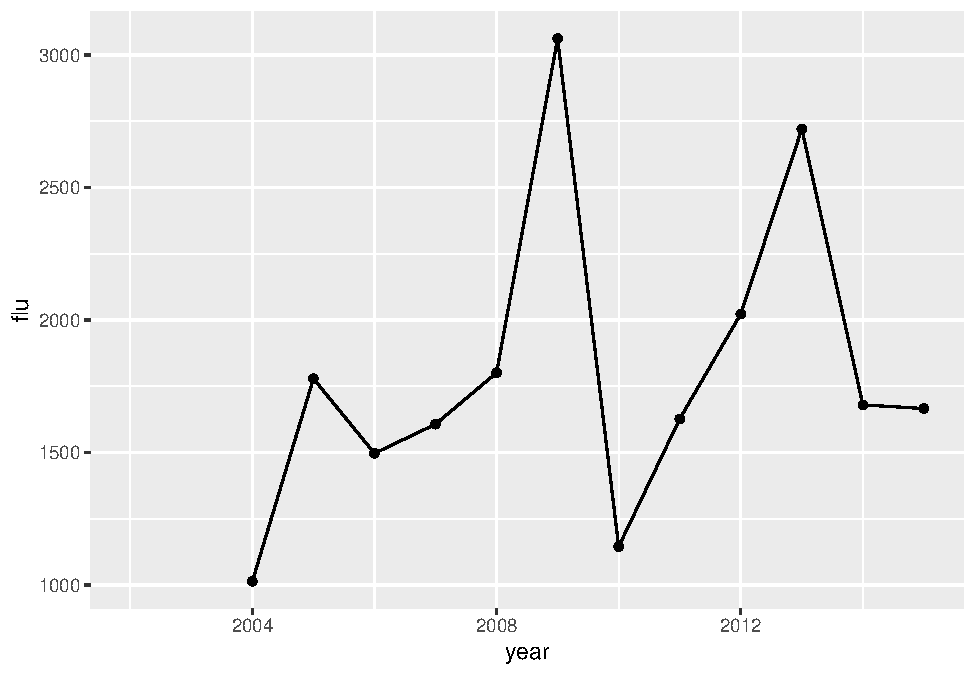
\includegraphics{Nexttry_files/figure-latex/unnamed-chunk-1-1.pdf}

\begin{Shaded}
\begin{Highlighting}[]
\NormalTok{alltogether }\SpecialCharTok{\%\textgreater{}\%} \FunctionTok{filter}\NormalTok{(country }\SpecialCharTok{==} \StringTok{"Argentina"}\NormalTok{) }\SpecialCharTok{\%\textgreater{}\%}
  \FunctionTok{ggplot}\NormalTok{() }\SpecialCharTok{+} 
  \FunctionTok{geom\_line}\NormalTok{(}\FunctionTok{aes}\NormalTok{(}\AttributeTok{y =}\NormalTok{ dengue,}\AttributeTok{x=}\NormalTok{year, }\AttributeTok{colour =} \StringTok{"green"}\NormalTok{),) }\SpecialCharTok{+} 
  \FunctionTok{geom\_line}\NormalTok{(}\FunctionTok{aes}\NormalTok{(}\AttributeTok{y =}\NormalTok{ flu,}\AttributeTok{x=}\NormalTok{year, }\AttributeTok{colour =} \StringTok{"red"}\NormalTok{))}
\end{Highlighting}
\end{Shaded}

\begin{verbatim}
## Warning: Removed 2 row(s) containing missing values (geom_path).
\end{verbatim}

\begin{verbatim}
## Warning: Removed 2 row(s) containing missing values (geom_path).
\end{verbatim}

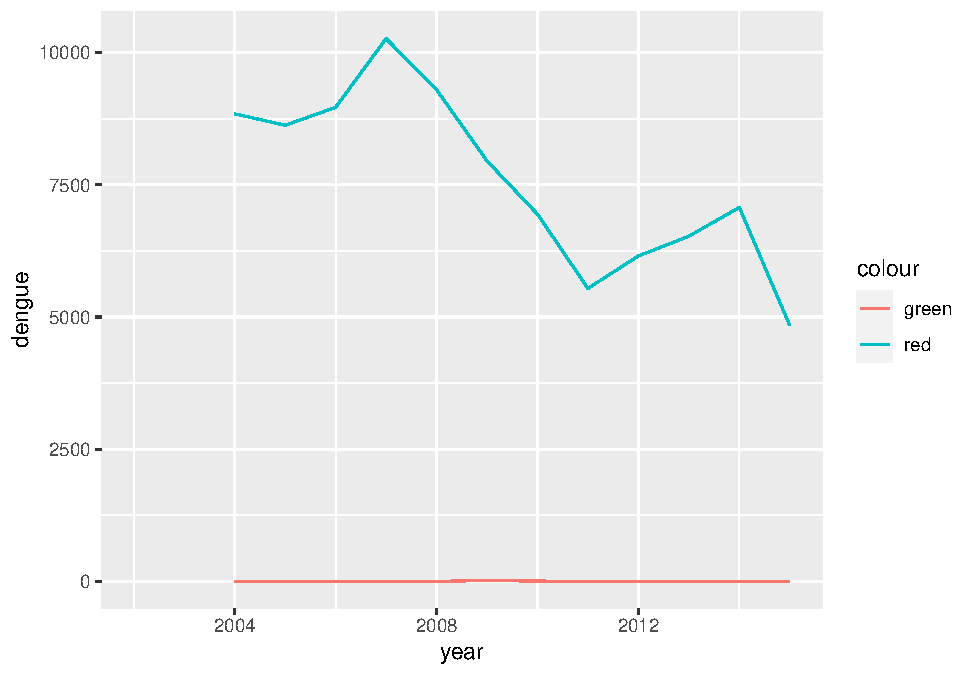
\includegraphics{Nexttry_files/figure-latex/unnamed-chunk-1-2.pdf}

\begin{Shaded}
\begin{Highlighting}[]
\FunctionTok{ggplot}\NormalTok{(}\AttributeTok{data =}\NormalTok{ alltogether, }\FunctionTok{aes}\NormalTok{(}\AttributeTok{x =}\NormalTok{ continent, }\AttributeTok{y =}\NormalTok{ flu)) }\SpecialCharTok{+}
  \FunctionTok{geom\_boxplot}\NormalTok{(}\FunctionTok{aes}\NormalTok{(}\AttributeTok{fill =}\NormalTok{ continent))}
\end{Highlighting}
\end{Shaded}

\begin{verbatim}
## Warning: Removed 72 rows containing non-finite values (stat_boxplot).
\end{verbatim}

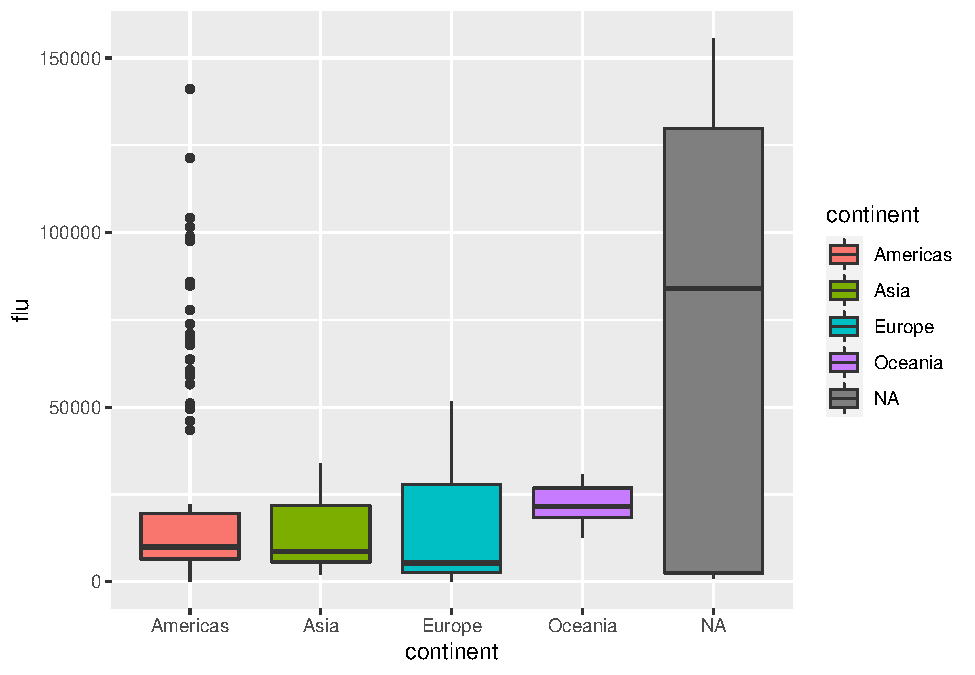
\includegraphics{Nexttry_files/figure-latex/unnamed-chunk-1-3.pdf}

\begin{Shaded}
\begin{Highlighting}[]
\FunctionTok{shapiro.test}\NormalTok{(alltogether}\SpecialCharTok{$}\NormalTok{fertility)}
\end{Highlighting}
\end{Shaded}

\begin{verbatim}
## 
##  Shapiro-Wilk normality test
## 
## data:  alltogether$fertility
## W = 0.84528, p-value < 2.2e-16
\end{verbatim}

\begin{Shaded}
\begin{Highlighting}[]
\FunctionTok{shapiro.test}\NormalTok{(alltogether}\SpecialCharTok{$}\NormalTok{flu)}
\end{Highlighting}
\end{Shaded}

\begin{verbatim}
## 
##  Shapiro-Wilk normality test
## 
## data:  alltogether$flu
## W = 0.70363, p-value < 2.2e-16
\end{verbatim}

\begin{Shaded}
\begin{Highlighting}[]
\FunctionTok{shapiro.test}\NormalTok{(alltogether}\SpecialCharTok{$}\NormalTok{dengue)}
\end{Highlighting}
\end{Shaded}

\begin{verbatim}
## 
##  Shapiro-Wilk normality test
## 
## data:  alltogether$dengue
## W = 0.91218, p-value = 0.0009743
\end{verbatim}

\begin{Shaded}
\begin{Highlighting}[]
\FunctionTok{shapiro.test}\NormalTok{(alltogether}\SpecialCharTok{$}\NormalTok{infant\_mortality)}
\end{Highlighting}
\end{Shaded}

\begin{verbatim}
## 
##  Shapiro-Wilk normality test
## 
## data:  alltogether$infant_mortality
## W = 0.75988, p-value < 2.2e-16
\end{verbatim}

\begin{Shaded}
\begin{Highlighting}[]
\FunctionTok{shapiro.test}\NormalTok{(alltogether}\SpecialCharTok{$}\NormalTok{life\_expectancy)}
\end{Highlighting}
\end{Shaded}

\begin{verbatim}
## 
##  Shapiro-Wilk normality test
## 
## data:  alltogether$life_expectancy
## W = 0.93264, p-value = 9.214e-12
\end{verbatim}

\begin{Shaded}
\begin{Highlighting}[]
\FunctionTok{shapiro.test}\NormalTok{(alltogether}\SpecialCharTok{$}\NormalTok{gdp)}
\end{Highlighting}
\end{Shaded}

\begin{verbatim}
## 
##  Shapiro-Wilk normality test
## 
## data:  alltogether$gdp
## W = 0.53327, p-value < 2.2e-16
\end{verbatim}

\begin{Shaded}
\begin{Highlighting}[]
\FunctionTok{shapiro.test}\NormalTok{(alltogether}\SpecialCharTok{$}\NormalTok{population)}
\end{Highlighting}
\end{Shaded}

\begin{verbatim}
## 
##  Shapiro-Wilk normality test
## 
## data:  alltogether$population
## W = 0.74646, p-value < 2.2e-16
\end{verbatim}

\hypertarget{my-own-package}{%
\chapter{My own package}\label{my-own-package}}

\hypertarget{parameters}{%
\chapter{Parameters}\label{parameters}}

\hypertarget{looking-ahead}{%
\chapter{Looking ahead}\label{looking-ahead}}

\hypertarget{appendix}{%
\chapter{Appendix}\label{appendix}}

\textbf{This code belongs to chapter 3}
R code for:
L?pez Steinmetz L.C., Dutto Florio M.A., Leyes C.A., Fong S.B., Rigalli A. \& Godoy J.C.
Levels and predictors of depression, anxiety, and suicidal risk during COVID-19 pandemic in Argentina: The impacts of quarantine extensions on mental health state.

\begin{Shaded}
\begin{Highlighting}[]
\FunctionTok{library}\NormalTok{(tidyverse)}
\FunctionTok{library}\NormalTok{(readxl)                            }
\CommentTok{\# Load the dataset:}
\NormalTok{table}\OtherTok{\textless{}{-}}\FunctionTok{read\_excel}\NormalTok{(}\StringTok{"data/Peer/dataset.xlsx"}\NormalTok{)}
\FunctionTok{summary}\NormalTok{(table)}
\end{Highlighting}
\end{Shaded}

\begin{verbatim}
##  SUB PERIODS         EDUCATION           PROVINCE             SEX           
##  Length:1100        Length:1100        Length:1100        Length:1100       
##  Class :character   Class :character   Class :character   Class :character  
##  Mode  :character   Mode  :character   Mode  :character   Mode  :character  
##                                                                             
##                                                                             
##                                                                             
##       AGE        MENTAL DISORDER HISTORY SUIC ATTEMPT HISTORY
##  Min.   :17.00   Length:1100             Length:1100         
##  1st Qu.:23.00   Class :character        Class :character    
##  Median :28.00   Mode  :character        Mode  :character    
##  Mean   :31.45                                               
##  3rd Qu.:37.00                                               
##  Max.   :76.00                                               
##  LIVING WITH SOMEBODY ECONOMIC INCOME      DEPRESSION     SUIC RISK    
##  Length:1100          Length:1100        Min.   : 0.0   Min.   : 0.00  
##  Class :character     Class :character   1st Qu.: 8.0   1st Qu.:18.00  
##  Mode  :character     Mode  :character   Median :13.0   Median :27.00  
##                                          Mean   :15.7   Mean   :30.32  
##                                          3rd Qu.:22.0   3rd Qu.:40.00  
##                                          Max.   :60.0   Max.   :89.00  
##  ANXIETY STATE   ANXIETY TRAIT 
##  Min.   : 1.00   Min.   : 0.0  
##  1st Qu.:21.00   1st Qu.:18.0  
##  Median :31.00   Median :26.0  
##  Mean   :31.78   Mean   :26.9  
##  3rd Qu.:42.00   3rd Qu.:36.0  
##  Max.   :66.00   Max.   :59.0
\end{verbatim}

\begin{Shaded}
\begin{Highlighting}[]
\DocumentationTok{\#\#\#\#\#\# SUB{-}TITLE: METHODS \textgreater{} Sample and procedure}
\CommentTok{\# SAMPLE N = 1100}

\CommentTok{\# Distribution by sex:}
\FunctionTok{table}\NormalTok{(table}\SpecialCharTok{$}\NormalTok{SEX)}
\end{Highlighting}
\end{Shaded}

\begin{verbatim}
## 
##   man woman 
##   217   883
\end{verbatim}

\begin{Shaded}
\begin{Highlighting}[]
\CommentTok{\# Absolute frequencies: Men = 217, Women = 883}
\FunctionTok{prop.table}\NormalTok{(}\FunctionTok{table}\NormalTok{(table}\SpecialCharTok{$}\NormalTok{SEX))}\SpecialCharTok{*}\DecValTok{100}
\end{Highlighting}
\end{Shaded}

\begin{verbatim}
## 
##      man    woman 
## 19.72727 80.27273
\end{verbatim}

\begin{Shaded}
\begin{Highlighting}[]
\CommentTok{\# Percentages: Men = 19.72727\%, Women = 80.27273\%}

\CommentTok{\# Central tendency measures by age (entire sample)}
\CommentTok{\# Mean}
\FunctionTok{mean}\NormalTok{(table}\SpecialCharTok{$}\NormalTok{AGE)}
\end{Highlighting}
\end{Shaded}

\begin{verbatim}
## [1] 31.45273
\end{verbatim}

\begin{Shaded}
\begin{Highlighting}[]
\CommentTok{\# Age: mean = 31.45273}

\CommentTok{\# Standard deviation (sd)}
\FunctionTok{sd}\NormalTok{(table}\SpecialCharTok{$}\NormalTok{AGE)}
\end{Highlighting}
\end{Shaded}

\begin{verbatim}
## [1] 11.7824
\end{verbatim}

\begin{Shaded}
\begin{Highlighting}[]
\CommentTok{\# Age: sd = 11.7824}

\CommentTok{\# Standard error (sem)}
\FunctionTok{library}\NormalTok{(}\StringTok{"plotrix"}\NormalTok{)}
\FunctionTok{std.error}\NormalTok{(table}\SpecialCharTok{$}\NormalTok{AGE)}
\end{Highlighting}
\end{Shaded}

\begin{verbatim}
## [1] 0.3552526
\end{verbatim}

\begin{Shaded}
\begin{Highlighting}[]
\CommentTok{\# Age: sem = 0.3552526}

\CommentTok{\# median}
\FunctionTok{median}\NormalTok{(table}\SpecialCharTok{$}\NormalTok{AGE)}
\end{Highlighting}
\end{Shaded}

\begin{verbatim}
## [1] 28
\end{verbatim}

\begin{Shaded}
\begin{Highlighting}[]
\CommentTok{\# Age: median = 28}


\DocumentationTok{\#\#\#\#\#\# SUB{-}TITLE: METHODS \textgreater{} Data analysis}

\CommentTok{\# To test Skewness and Kurtosis \# Criteria: range of acceptable values or near to {-}3 and +3 (Brown, 2006).}
\CommentTok{\# Reference: Brown, T. A. (2006). Confirmatory factor analysis for applied research. New York: Guilford Press.}

\FunctionTok{library}\NormalTok{(moments)}

\CommentTok{\# DEPRESSION}
\FunctionTok{skewness}\NormalTok{(table}\SpecialCharTok{$}\NormalTok{DEPRESSION) }
\end{Highlighting}
\end{Shaded}

\begin{verbatim}
## [1] 1.014193
\end{verbatim}

\begin{Shaded}
\begin{Highlighting}[]
\CommentTok{\# skewness DEPRESSION = 1.014193}
\FunctionTok{kurtosis}\NormalTok{(table}\SpecialCharTok{$}\NormalTok{DEPRESSION)}
\end{Highlighting}
\end{Shaded}

\begin{verbatim}
## [1] 3.789272
\end{verbatim}

\begin{Shaded}
\begin{Highlighting}[]
\CommentTok{\# kurtosis DEPRESSION = 3.789272}

\NormalTok{table }\OtherTok{\textless{}{-}} \FunctionTok{rename}\NormalTok{(table,  }\StringTok{"ANXIETY\_STATE"} \OtherTok{=} \StringTok{"ANXIETY STATE"}\NormalTok{,}
                \StringTok{"ANXIETY\_TRAIT"} \OtherTok{=} \StringTok{"ANXIETY TRAIT"}\NormalTok{,}
                \StringTok{"SUIC\_RISK"} \OtherTok{=} \StringTok{"SUIC RISK"}\NormalTok{,}
                \StringTok{"SUB\_PERIODS"} \OtherTok{=} \StringTok{"SUB PERIODS"}\NormalTok{,}
                \StringTok{"MENTAL\_DISORDER\_HISTORY"} \OtherTok{=} \StringTok{"MENTAL DISORDER HISTORY"}\NormalTok{,}
                \StringTok{"SUIC\_ATTEMPT\_HISTORY"} \OtherTok{=} \StringTok{"SUIC ATTEMPT HISTORY"}\NormalTok{,}
                \StringTok{"LIVING\_WITH\_SOMEBODY"} \OtherTok{=} \StringTok{"LIVING WITH SOMEBODY"}\NormalTok{,}
                \StringTok{"ECONOMIC\_INCOME"} \OtherTok{=} \StringTok{"ECONOMIC INCOME"}\NormalTok{)}
\CommentTok{\# ANXIETY STATE}
\FunctionTok{skewness}\NormalTok{(table}\SpecialCharTok{$}\NormalTok{ANXIETY\_STATE) }
\end{Highlighting}
\end{Shaded}

\begin{verbatim}
## [1] 0.2010007
\end{verbatim}

\begin{Shaded}
\begin{Highlighting}[]
\CommentTok{\# skewness ANXIETY STATE = 0.2010007}
\FunctionTok{kurtosis}\NormalTok{(table}\SpecialCharTok{$}\NormalTok{ANXIETY\_STATE)}
\end{Highlighting}
\end{Shaded}

\begin{verbatim}
## [1] 2.341017
\end{verbatim}

\begin{Shaded}
\begin{Highlighting}[]
\CommentTok{\# kurtosis ANXIETY STATE = 2.341017}

\CommentTok{\# ANXIETY TRAIT}
\FunctionTok{skewness}\NormalTok{(table}\SpecialCharTok{$}\NormalTok{ANXIETY\_TRAIT) }
\end{Highlighting}
\end{Shaded}

\begin{verbatim}
## [1] 0.2401163
\end{verbatim}

\begin{Shaded}
\begin{Highlighting}[]
\CommentTok{\# skewness ANXIETY TRAIT = 0.2401163}
\FunctionTok{kurtosis}\NormalTok{(table}\SpecialCharTok{$}\NormalTok{ANXIETY\_TRAIT)}
\end{Highlighting}
\end{Shaded}

\begin{verbatim}
## [1] 2.354038
\end{verbatim}

\begin{Shaded}
\begin{Highlighting}[]
\CommentTok{\# kurtosis ANXIETY TRAIT = 2.354038}

\CommentTok{\# SUICIDAL RISK}
\FunctionTok{skewness}\NormalTok{(table}\SpecialCharTok{$}\NormalTok{SUIC\_RISK) }
\end{Highlighting}
\end{Shaded}

\begin{verbatim}
## [1] 0.8331517
\end{verbatim}

\begin{Shaded}
\begin{Highlighting}[]
\CommentTok{\# skewness SUICIDAL RISK = 0.8331517}
\FunctionTok{kurtosis}\NormalTok{(table}\SpecialCharTok{$}\NormalTok{SUIC\_RISK)}
\end{Highlighting}
\end{Shaded}

\begin{verbatim}
## [1] 3.193105
\end{verbatim}

\begin{Shaded}
\begin{Highlighting}[]
\CommentTok{\# kurtosis SUICIDAL RISK = 3.193105}



\CommentTok{\# For addresing the first aim, we divided the entire sample into three groups: }
\FunctionTok{table}\NormalTok{(table}\SpecialCharTok{$}\NormalTok{SUB\_PERIODS)}
\end{Highlighting}
\end{Shaded}

\begin{verbatim}
## 
##    1. EXT POST 2./3. EXT POST    4. EXT POST 
##            362            239            499
\end{verbatim}

\begin{Shaded}
\begin{Highlighting}[]
\CommentTok{\# first quarantine extension (1. EXT POST) = 362}
\CommentTok{\# second and third quarantine extensions (2. EXT POST) = 239}
\CommentTok{\# fourth quarantine extension (3. EXT POST) = 499}



\DocumentationTok{\#\#\#\#\#\#\#\#\#\#\#\#\#\#\#\#\#\#\#\#\#\#\#\#\#\#\#\#\#\#\#\#\#\#\#\#\#\#\#\#\#\#\#\#\#\#\#\#\#\#\#\#\#\#\#\#\#\#\#\#\#\#\#\#\#\#\#\#\#\#\#\#\#\#\#\#\#\#\#\#\#\#\#\#\#\#\#\#\#\#\#}
\DocumentationTok{\#\#\#\#\#\#\#\#\#\#\#\#\#\#\#\#\#\#\#\#\#\#\#\#\#\#\#\#\#\#\#\#\#\#\#\#\#\#\#\#\# RESULTS \#\#\#\#\#\#\#\#\#\#\#\#\#\#\#\#\#\#\#\#\#\#\#\#\#\#\#\#\#\#\#\#\#\#\#\#\#\#\#\#\#}
\DocumentationTok{\#\#\#\#\#\#\#\#\#\#\#\#\#\#\#\#\#\#\#\#\#\#\#\#\#\#\#\#\#\#\#\#\#\#\#\#\#\#\#\#\#\#\#\#\#\#\#\#\#\#\#\#\#\#\#\#\#\#\#\#\#\#\#\#\#\#\#\#\#\#\#\#\#\#\#\#\#\#\#\#\#\#\#\#\#\#\#\#\#\#\#}

\DocumentationTok{\#\#\#\#\#\#\#\#\#\#\#\#\#\#\#\#\#\#\#\#\#\#\#\#\#\#\#\#\#\#\#\#\#\#\#\#\#\#\#\#\#\#\#\#\#\#\#\#\#\#\#\#\#\#\#\#\#\#\#\#\#\#\#\#\#\#\#\#\#\#\#\#\#\#\#\#\#\#\#\#\#\#\#\#\#\#\#\#\#\#\#}
\DocumentationTok{\#\#\#\#\#\#\#\#\#\#\#\#\#\#\#\#\#\#\#\#\#\#\#\#\#\#\#\#\#\#\#\#\#\#\#\#\#\#\#\#\# AIM 1 \#\#\#\#\#\#\#\#\#\#\#\#\#\#\#\#\#\#\#\#\#\#\#\#\#\#\#\#\#\#\#\#\#\#\#\#\#\#\#\#\#\#\#}

\CommentTok{\# Load this library for computing effect sizes:}
\FunctionTok{library}\NormalTok{(sjstats)}

\DocumentationTok{\#\#\#\#\#\#\#\#\#\#\#\#\#\#\#\#\#\#\#\#\#\#\#\#\#\#\#\#\#\#\#\#\#\#\#\#\#\#\#\#\#\#\#\#\#\#\#\#\#\#\#\#\#\#\#\#\#\#\#\#\#\#\#\#\#\#\#\#\#\#\#\#\#\#\#\#\#\#\#\#\#\#\#\#\#\#\#\#\#\#\#\#\#}
\DocumentationTok{\#\#\# Differences in specific mental health state indicators by three sub{-}periods of quarantine}

\CommentTok{\# 1. EXT POST = first quarantine extension}
\CommentTok{\# 2./3. EXT POST = second/third quarantine extensions}
\CommentTok{\# 4. EXT POST = fourth quarantine extension}

\CommentTok{\# DEPRESSION}
\NormalTok{anovatempdepr }\OtherTok{\textless{}{-}} \FunctionTok{aov}\NormalTok{(table}\SpecialCharTok{$}\NormalTok{DEPRESSION}\SpecialCharTok{\textasciitilde{}}\NormalTok{table}\SpecialCharTok{$}\NormalTok{SUB\_PERIODS)}
\NormalTok{anovatempdepr}
\end{Highlighting}
\end{Shaded}

\begin{verbatim}
## Call:
##    aov(formula = table$DEPRESSION ~ table$SUB_PERIODS)
## 
## Terms:
##                 table$SUB_PERIODS Residuals
## Sum of Squares            2630.12 132802.86
## Deg. of Freedom                 2      1097
## 
## Residual standard error: 11.00273
## Estimated effects may be unbalanced
\end{verbatim}

\begin{Shaded}
\begin{Highlighting}[]
\FunctionTok{summary}\NormalTok{(anovatempdepr)}
\end{Highlighting}
\end{Shaded}

\begin{verbatim}
##                     Df Sum Sq Mean Sq F value   Pr(>F)    
## table$SUB_PERIODS    2   2630  1315.1   10.86 2.13e-05 ***
## Residuals         1097 132803   121.1                     
## ---
## Signif. codes:  0 '***' 0.001 '**' 0.01 '*' 0.05 '.' 0.1 ' ' 1
\end{verbatim}

\begin{Shaded}
\begin{Highlighting}[]
\FunctionTok{plot}\NormalTok{(anovatempdepr)}
\end{Highlighting}
\end{Shaded}

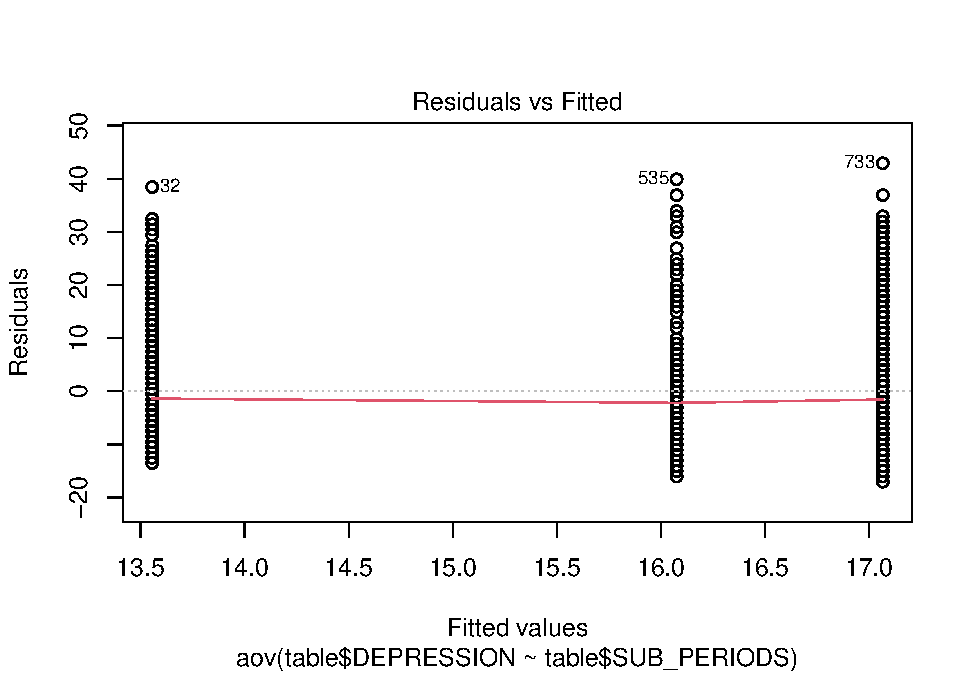
\includegraphics{Nexttry_files/figure-latex/unnamed-chunk-2-1.pdf} 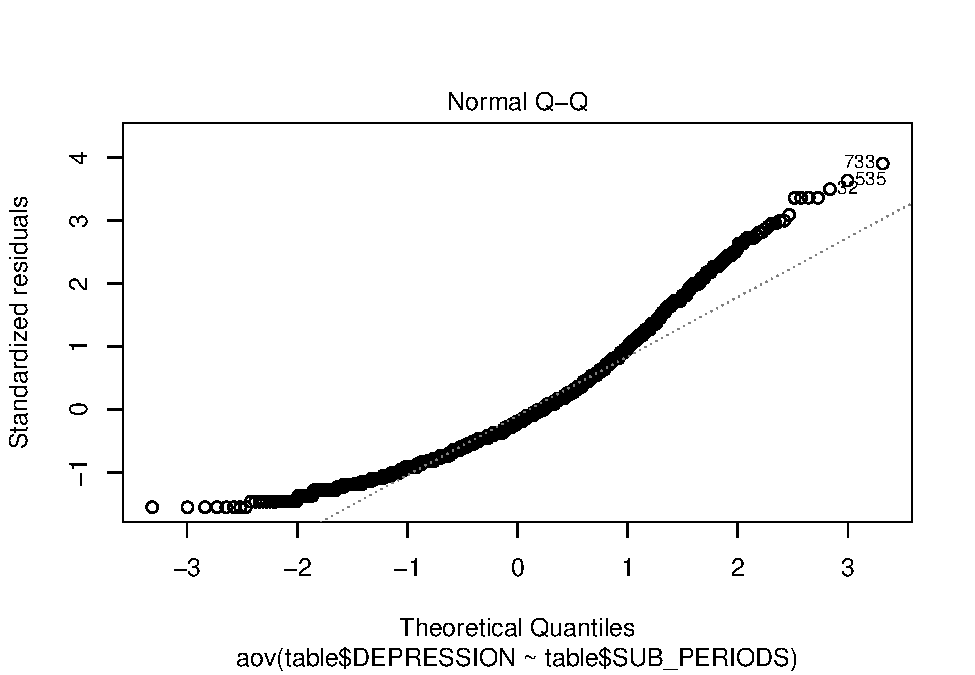
\includegraphics{Nexttry_files/figure-latex/unnamed-chunk-2-2.pdf} 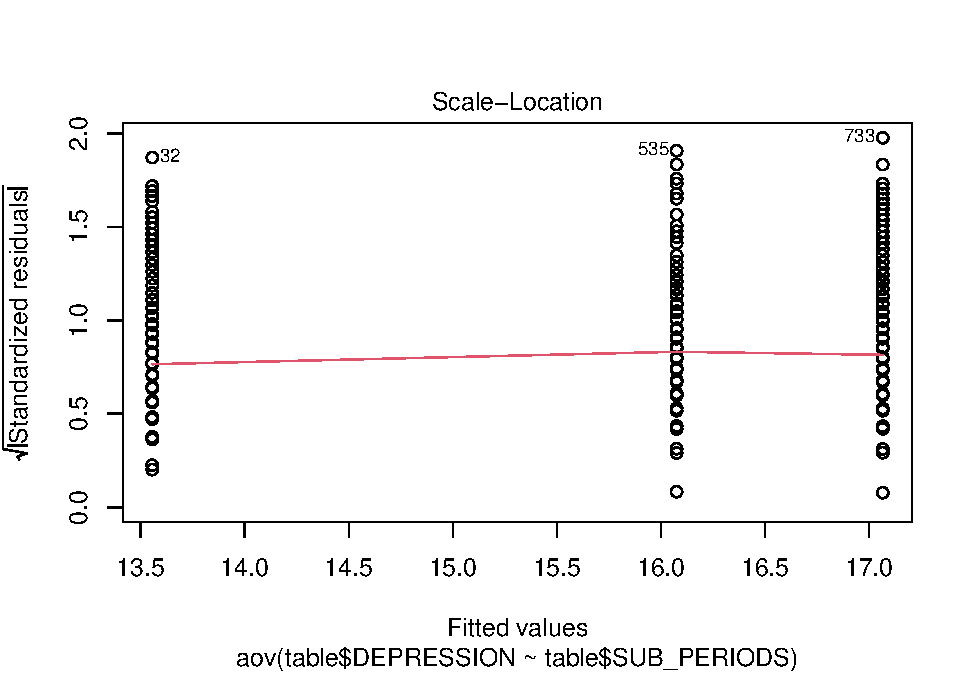
\includegraphics{Nexttry_files/figure-latex/unnamed-chunk-2-3.pdf} 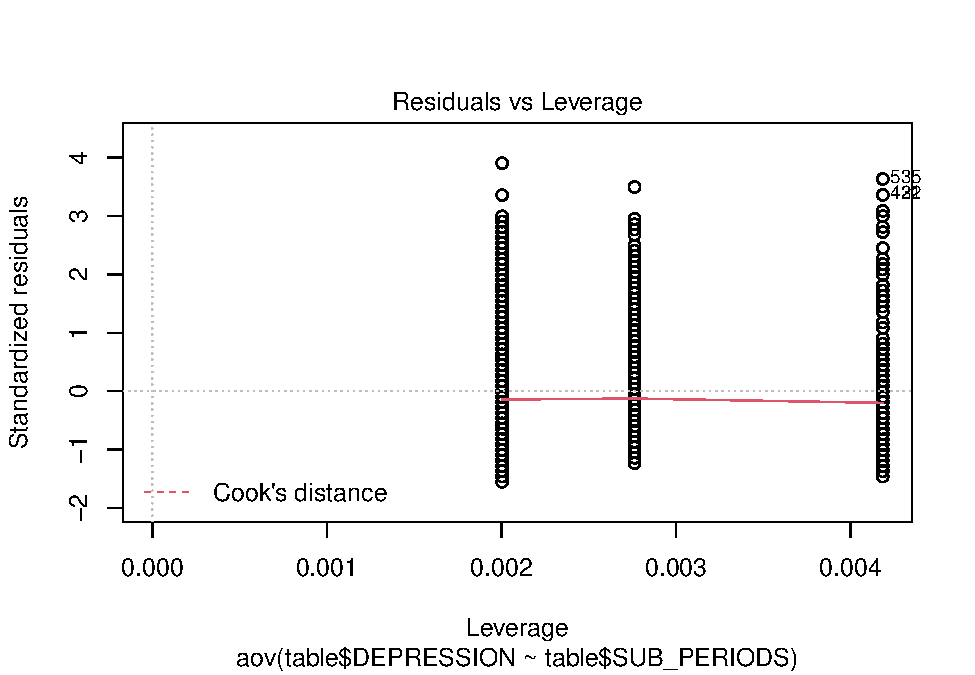
\includegraphics{Nexttry_files/figure-latex/unnamed-chunk-2-4.pdf}

\begin{Shaded}
\begin{Highlighting}[]
\FunctionTok{pairwise.t.test}\NormalTok{(}\AttributeTok{x =}\NormalTok{ table}\SpecialCharTok{$}\NormalTok{DEPRESSION, }\AttributeTok{g =}\NormalTok{ table}\SpecialCharTok{$}\NormalTok{SUB\_PERIODS, }\AttributeTok{p.adjust.method =} \StringTok{"bonferroni"}\NormalTok{, }\AttributeTok{pool.sd =} \ConstantTok{TRUE}\NormalTok{, }\AttributeTok{paired =} \ConstantTok{FALSE}\NormalTok{, }\AttributeTok{alternative =} \StringTok{"two.sided"}\NormalTok{)}
\end{Highlighting}
\end{Shaded}

\begin{verbatim}
## 
##  Pairwise comparisons using t tests with pooled SD 
## 
## data:  table$DEPRESSION and table$SUB_PERIODS 
## 
##                1. EXT POST 2./3. EXT POST
## 2./3. EXT POST 0.018       -             
## 4. EXT POST    1.3e-05     0.758         
## 
## P value adjustment method: bonferroni
\end{verbatim}

\begin{Shaded}
\begin{Highlighting}[]
\CommentTok{\# significant differences}
\CommentTok{\# 2./3. EXT POST{-}1. EXT POST p adj 0.018}
\CommentTok{\# 4. EXT POST{-}1. EXT POST p adj 1.3e{-}05}
\CommentTok{\#effectsize::cohens\_f(anovatempdepr, ci = 0.95, partial = TRUE, type = 1)}

\FunctionTok{tapply}\NormalTok{(table}\SpecialCharTok{$}\NormalTok{DEPRESSION,}\FunctionTok{factor}\NormalTok{(table}\SpecialCharTok{$}\NormalTok{SUB\_PERIODS),mean)}
\end{Highlighting}
\end{Shaded}

\begin{verbatim}
##    1. EXT POST 2./3. EXT POST    4. EXT POST 
##       13.55525       16.07531       17.06613
\end{verbatim}

\begin{Shaded}
\begin{Highlighting}[]
\FunctionTok{tapply}\NormalTok{(table}\SpecialCharTok{$}\NormalTok{DEPRESSION,}\FunctionTok{factor}\NormalTok{(table}\SpecialCharTok{$}\NormalTok{SUB\_PERIODS),std.error)}
\end{Highlighting}
\end{Shaded}

\begin{verbatim}
##    1. EXT POST 2./3. EXT POST    4. EXT POST 
##      0.5304822      0.7764039      0.4984415
\end{verbatim}

\begin{Shaded}
\begin{Highlighting}[]
\FunctionTok{library}\NormalTok{(gplots)}
\end{Highlighting}
\end{Shaded}

\begin{verbatim}
## 
## Attaching package: 'gplots'
\end{verbatim}

\begin{verbatim}
## The following object is masked from 'package:plotrix':
## 
##     plotCI
\end{verbatim}

\begin{verbatim}
## The following object is masked from 'package:stats':
## 
##     lowess
\end{verbatim}

\begin{Shaded}
\begin{Highlighting}[]
\CommentTok{\# Figure S1 (Supplementary material)}
\FunctionTok{plotmeans}\NormalTok{(table}\SpecialCharTok{$}\NormalTok{DEPRESSION}\SpecialCharTok{\textasciitilde{}}\NormalTok{table}\SpecialCharTok{$}\NormalTok{SUB\_PERIODS, }\AttributeTok{main=}\StringTok{"Fig. S1. Depression by quarantine sub{-}periods. Mean plot with 95\% Confidence Interval"}\NormalTok{, }\AttributeTok{cex.main =} \FloatTok{0.8}\NormalTok{, }\AttributeTok{ylab =} \StringTok{"Depression"}\NormalTok{, }\AttributeTok{xlab =} \StringTok{"Quarantine\textquotesingle{}s sub periods"}\NormalTok{)}
\end{Highlighting}
\end{Shaded}

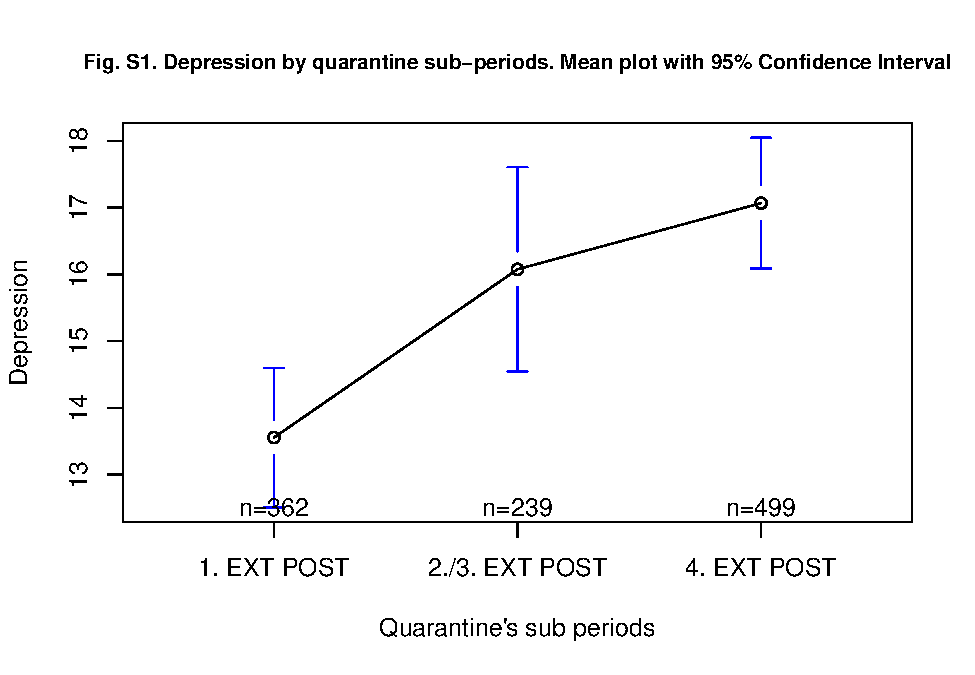
\includegraphics{Nexttry_files/figure-latex/unnamed-chunk-2-5.pdf}

\begin{Shaded}
\begin{Highlighting}[]
\FunctionTok{mean}\NormalTok{(table}\SpecialCharTok{$}\NormalTok{DEPRESSION) }\CommentTok{\# mean = 15.69545}
\end{Highlighting}
\end{Shaded}

\begin{verbatim}
## [1] 15.69545
\end{verbatim}

\begin{Shaded}
\begin{Highlighting}[]
\FunctionTok{std.error}\NormalTok{(table}\SpecialCharTok{$}\NormalTok{DEPRESSION) }\CommentTok{\# std. error = 0.3347087}
\end{Highlighting}
\end{Shaded}

\begin{verbatim}
## [1] 0.3347087
\end{verbatim}

\begin{Shaded}
\begin{Highlighting}[]
\CommentTok{\# Percentage distribution by cutoff score:}
\CommentTok{\# non clinically depressed:}
\FunctionTok{prop.table}\NormalTok{(}\FunctionTok{table}\NormalTok{(table}\SpecialCharTok{$}\NormalTok{DEPRESSION}\SpecialCharTok{\textless{}}\DecValTok{20}\NormalTok{,table}\SpecialCharTok{$}\NormalTok{SUB\_PERIODS))}\SpecialCharTok{*}\DecValTok{100}
\end{Highlighting}
\end{Shaded}

\begin{verbatim}
##        
##         1. EXT POST 2./3. EXT POST 4. EXT POST
##   FALSE    7.636364       6.727273   15.272727
##   TRUE    25.272727      15.000000   30.090909
\end{verbatim}

\begin{Shaded}
\begin{Highlighting}[]
\CommentTok{\# clinically depressed:}
\FunctionTok{prop.table}\NormalTok{(}\FunctionTok{table}\NormalTok{(table}\SpecialCharTok{$}\NormalTok{DEPRESSION}\SpecialCharTok{\textgreater{}=}\DecValTok{20}\NormalTok{,table}\SpecialCharTok{$}\NormalTok{SUB\_PERIODS))}\SpecialCharTok{*}\DecValTok{100}
\end{Highlighting}
\end{Shaded}

\begin{verbatim}
##        
##         1. EXT POST 2./3. EXT POST 4. EXT POST
##   FALSE   25.272727      15.000000   30.090909
##   TRUE     7.636364       6.727273   15.272727
\end{verbatim}

\begin{Shaded}
\begin{Highlighting}[]
\CommentTok{\# ANXIETY STATE}
\NormalTok{anovatempanxstate }\OtherTok{\textless{}{-}} \FunctionTok{aov}\NormalTok{(table}\SpecialCharTok{$}\NormalTok{ANXIETY\_STATE}\SpecialCharTok{\textasciitilde{}}\NormalTok{table}\SpecialCharTok{$}\NormalTok{SUB\_PERIODS)}
\NormalTok{anovatempanxstate}
\end{Highlighting}
\end{Shaded}

\begin{verbatim}
## Call:
##    aov(formula = table$ANXIETY_STATE ~ table$SUB_PERIODS)
## 
## Terms:
##                 table$SUB_PERIODS Residuals
## Sum of Squares             2824.4  227397.1
## Deg. of Freedom                 2      1097
## 
## Residual standard error: 14.39757
## Estimated effects may be unbalanced
\end{verbatim}

\begin{Shaded}
\begin{Highlighting}[]
\FunctionTok{summary}\NormalTok{(anovatempanxstate)}
\end{Highlighting}
\end{Shaded}

\begin{verbatim}
##                     Df Sum Sq Mean Sq F value  Pr(>F)   
## table$SUB_PERIODS    2   2824  1412.2   6.813 0.00115 **
## Residuals         1097 227397   207.3                   
## ---
## Signif. codes:  0 '***' 0.001 '**' 0.01 '*' 0.05 '.' 0.1 ' ' 1
\end{verbatim}

\begin{Shaded}
\begin{Highlighting}[]
\FunctionTok{plot}\NormalTok{(anovatempanxstate)}
\end{Highlighting}
\end{Shaded}

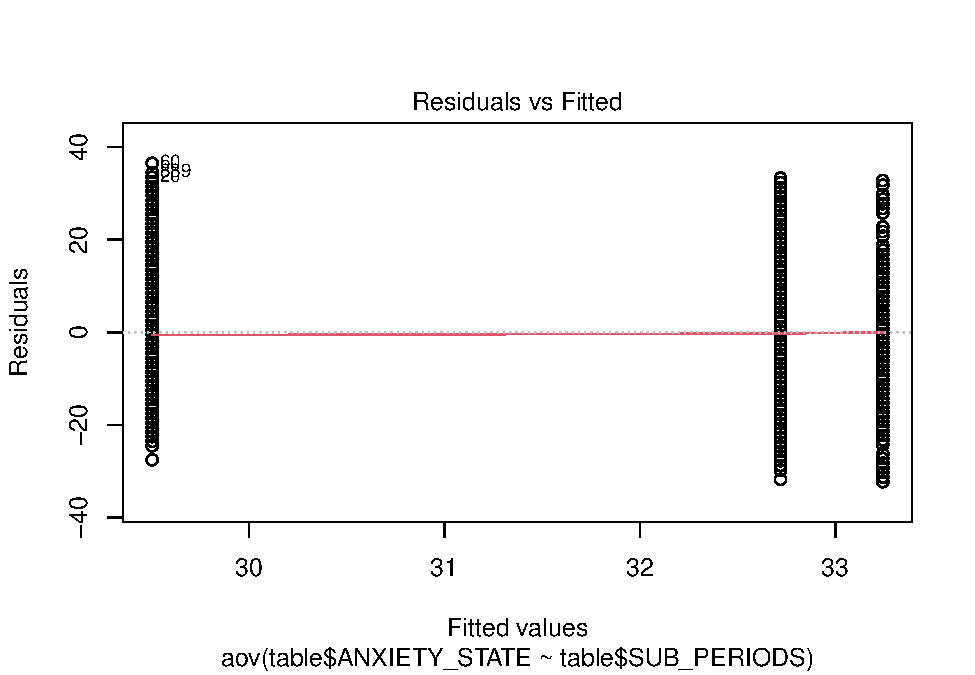
\includegraphics{Nexttry_files/figure-latex/unnamed-chunk-2-6.pdf} 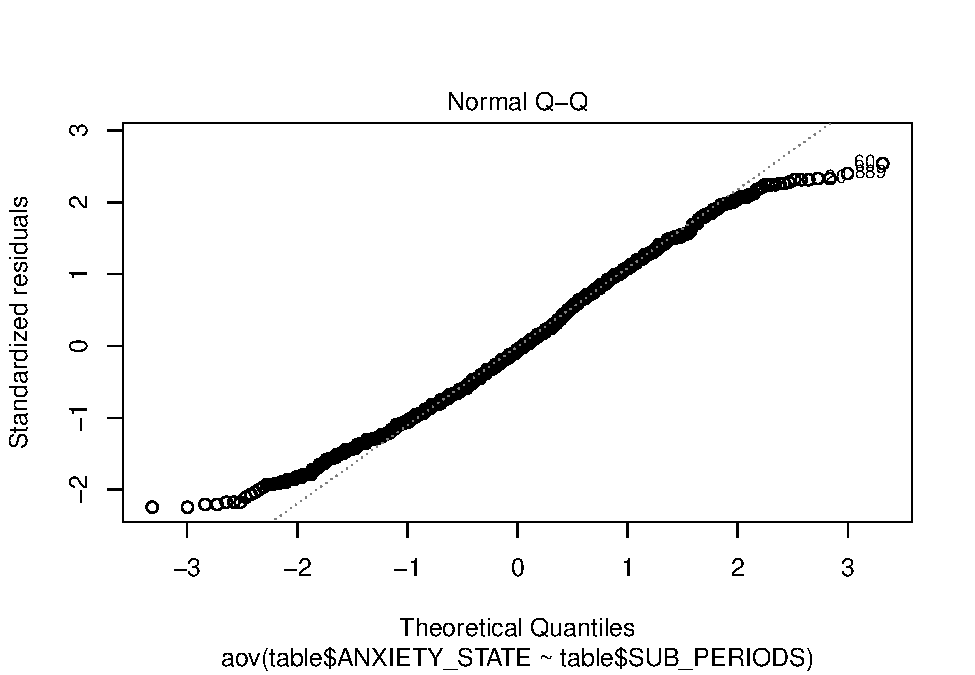
\includegraphics{Nexttry_files/figure-latex/unnamed-chunk-2-7.pdf} 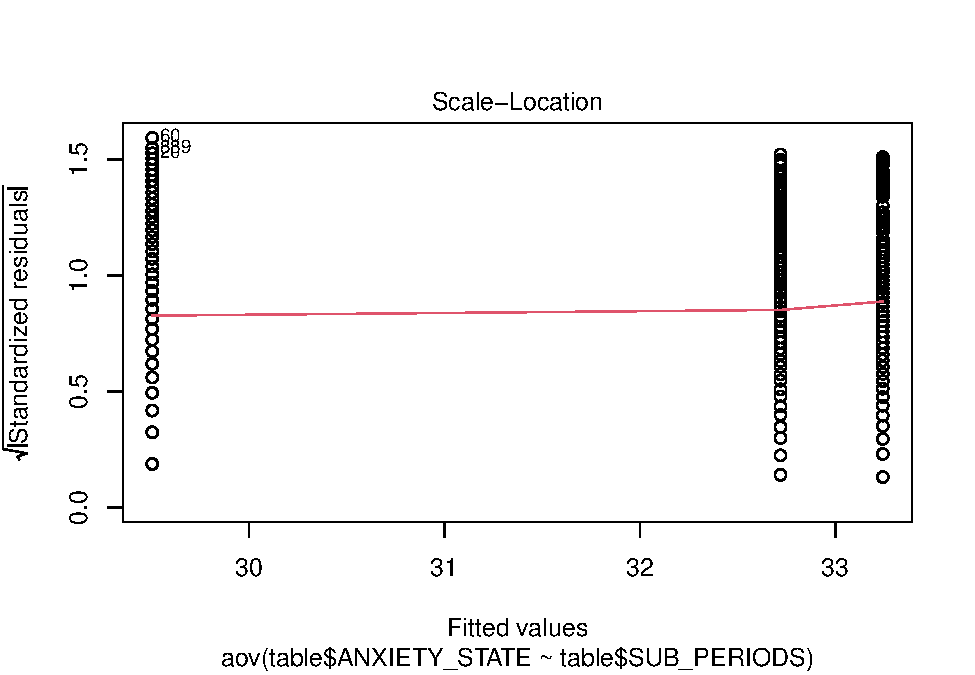
\includegraphics{Nexttry_files/figure-latex/unnamed-chunk-2-8.pdf} 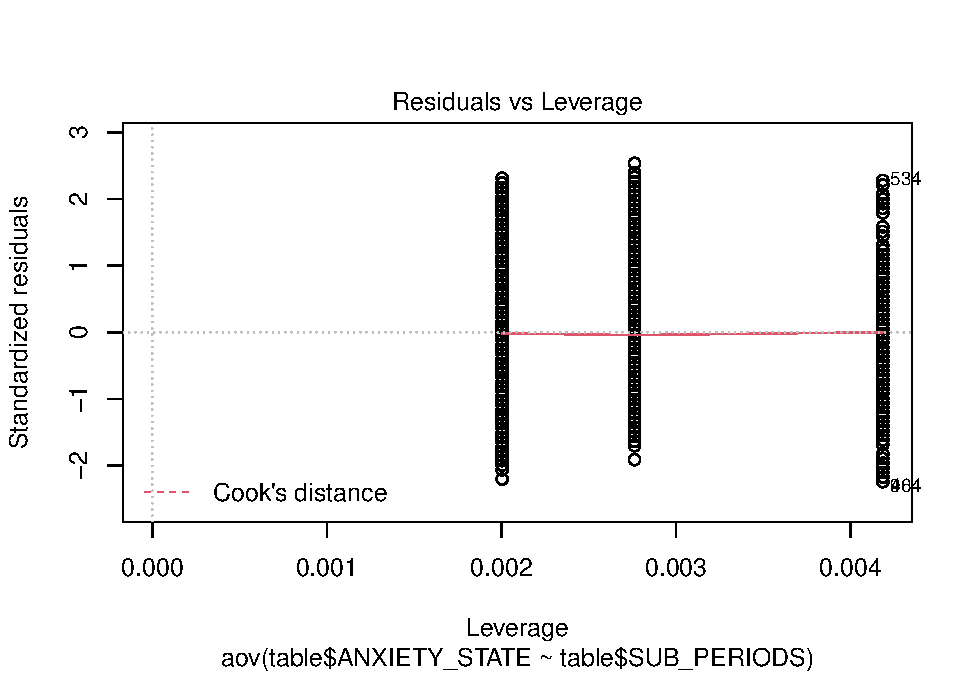
\includegraphics{Nexttry_files/figure-latex/unnamed-chunk-2-9.pdf}

\begin{Shaded}
\begin{Highlighting}[]
\FunctionTok{pairwise.t.test}\NormalTok{(}\AttributeTok{x =}\NormalTok{ table}\SpecialCharTok{$}\NormalTok{ANXIETY\_STATE, }\AttributeTok{g =}\NormalTok{ table}\SpecialCharTok{$}\NormalTok{SUB\_PERIODS, }\AttributeTok{p.adjust.method =} \StringTok{"bonferroni"}\NormalTok{, }\AttributeTok{pool.sd =} \ConstantTok{TRUE}\NormalTok{, }\AttributeTok{paired =} \ConstantTok{FALSE}\NormalTok{, }\AttributeTok{alternative =} \StringTok{"two.sided"}\NormalTok{)}
\end{Highlighting}
\end{Shaded}

\begin{verbatim}
## 
##  Pairwise comparisons using t tests with pooled SD 
## 
## data:  table$ANXIETY_STATE and table$SUB_PERIODS 
## 
##                1. EXT POST 2./3. EXT POST
## 2./3. EXT POST 0.0057      -             
## 4. EXT POST    0.0038      1.0000        
## 
## P value adjustment method: bonferroni
\end{verbatim}

\begin{Shaded}
\begin{Highlighting}[]
\CommentTok{\# significant differences}
\CommentTok{\# 2./3. EXT POST{-}1. EXT POST p adj 0.0057}
\CommentTok{\# 4. EXT POST{-}1. EXT POST p adj 0.0038}
\CommentTok{\#effectsize::cohens\_f(anovatempanxstate, ci = 0.95, partial = TRUE, type = 1)}

\FunctionTok{tapply}\NormalTok{(table}\SpecialCharTok{$}\NormalTok{ANXIETY\_STATE,}\FunctionTok{factor}\NormalTok{(table}\SpecialCharTok{$}\NormalTok{SUB\_PERIODS),mean)}
\end{Highlighting}
\end{Shaded}

\begin{verbatim}
##    1. EXT POST 2./3. EXT POST    4. EXT POST 
##       29.50552       33.24268       32.71944
\end{verbatim}

\begin{Shaded}
\begin{Highlighting}[]
\FunctionTok{tapply}\NormalTok{(table}\SpecialCharTok{$}\NormalTok{ANXIETY\_STATE,}\FunctionTok{factor}\NormalTok{(table}\SpecialCharTok{$}\NormalTok{SUB\_PERIODS),std.error)}
\end{Highlighting}
\end{Shaded}

\begin{verbatim}
##    1. EXT POST 2./3. EXT POST    4. EXT POST 
##      0.7206212      1.0085072      0.6396676
\end{verbatim}

\begin{Shaded}
\begin{Highlighting}[]
\CommentTok{\# Figure S2 (Supplementary material)}
\FunctionTok{plotmeans}\NormalTok{(table}\SpecialCharTok{$}\NormalTok{ANXIETY\_STATE}\SpecialCharTok{\textasciitilde{}}\NormalTok{table}\SpecialCharTok{$}\NormalTok{SUB\_PERIODS, }\AttributeTok{main=}\StringTok{"Fig. S2. State{-}Anxiety by quarantine sub{-}periods. Mean plot with 95\% Confidence Interval"}\NormalTok{, }\AttributeTok{cex.main =} \FloatTok{0.8}\NormalTok{, }\AttributeTok{ylab =} \StringTok{"State{-}Anxiety"}\NormalTok{, }\AttributeTok{xlab =} \StringTok{"Quarantine\textquotesingle{}s sub periods"}\NormalTok{)}
\end{Highlighting}
\end{Shaded}

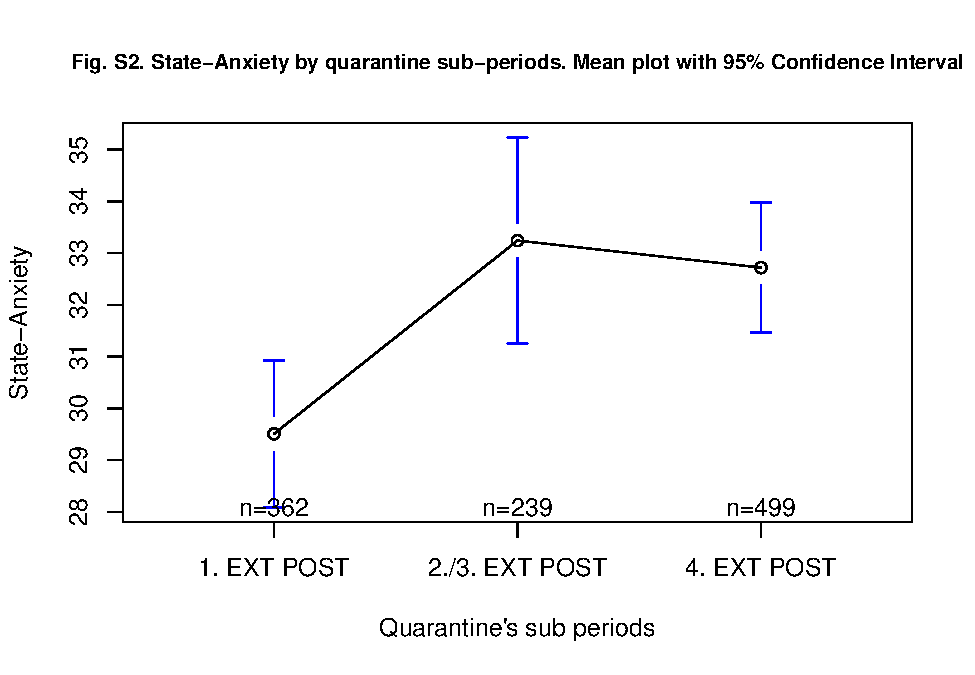
\includegraphics{Nexttry_files/figure-latex/unnamed-chunk-2-10.pdf}

\begin{Shaded}
\begin{Highlighting}[]
\FunctionTok{mean}\NormalTok{(table}\SpecialCharTok{$}\NormalTok{ANXIETY\_STATE) }\CommentTok{\# mean = 31.77545}
\end{Highlighting}
\end{Shaded}

\begin{verbatim}
## [1] 31.77545
\end{verbatim}

\begin{Shaded}
\begin{Highlighting}[]
\FunctionTok{std.error}\NormalTok{(table}\SpecialCharTok{$}\NormalTok{ANXIETY\_STATE) }\CommentTok{\# std. error = 0.436393}
\end{Highlighting}
\end{Shaded}

\begin{verbatim}
## [1] 0.436393
\end{verbatim}

\begin{Shaded}
\begin{Highlighting}[]
\CommentTok{\# low:}
\FunctionTok{prop.table}\NormalTok{(}\FunctionTok{table}\NormalTok{(table}\SpecialCharTok{$}\NormalTok{ANXIETY\_STATE}\SpecialCharTok{\textless{}}\DecValTok{32}\NormalTok{,table}\SpecialCharTok{$}\NormalTok{SUB\_PERIODS))}\SpecialCharTok{*}\DecValTok{100}
\end{Highlighting}
\end{Shaded}

\begin{verbatim}
##        
##         1. EXT POST 2./3. EXT POST 4. EXT POST
##   FALSE   13.636364      12.181818   22.727273
##   TRUE    19.272727       9.545455   22.636364
\end{verbatim}

\begin{Shaded}
\begin{Highlighting}[]
\CommentTok{\# high:}
\FunctionTok{prop.table}\NormalTok{(}\FunctionTok{table}\NormalTok{(table}\SpecialCharTok{$}\NormalTok{ANXIETY\_STATE}\SpecialCharTok{\textgreater{}=}\DecValTok{32}\NormalTok{,table}\SpecialCharTok{$}\NormalTok{SUB\_PERIODS))}\SpecialCharTok{*}\DecValTok{100}
\end{Highlighting}
\end{Shaded}

\begin{verbatim}
##        
##         1. EXT POST 2./3. EXT POST 4. EXT POST
##   FALSE   19.272727       9.545455   22.636364
##   TRUE    13.636364      12.181818   22.727273
\end{verbatim}

\begin{Shaded}
\begin{Highlighting}[]
\CommentTok{\# ANXIETY TRAIT}
\NormalTok{anovatempanxtrait }\OtherTok{\textless{}{-}} \FunctionTok{aov}\NormalTok{(table}\SpecialCharTok{$}\NormalTok{ANXIETY\_TRAIT}\SpecialCharTok{\textasciitilde{}}\NormalTok{table}\SpecialCharTok{$}\NormalTok{SUB\_PERIODS)}
\NormalTok{anovatempanxtrait}
\end{Highlighting}
\end{Shaded}

\begin{verbatim}
## Call:
##    aov(formula = table$ANXIETY_TRAIT ~ table$SUB_PERIODS)
## 
## Terms:
##                 table$SUB_PERIODS Residuals
## Sum of Squares            1306.59 160872.80
## Deg. of Freedom                 2      1097
## 
## Residual standard error: 12.10983
## Estimated effects may be unbalanced
\end{verbatim}

\begin{Shaded}
\begin{Highlighting}[]
\FunctionTok{summary}\NormalTok{(anovatempanxtrait)}
\end{Highlighting}
\end{Shaded}

\begin{verbatim}
##                     Df Sum Sq Mean Sq F value Pr(>F)  
## table$SUB_PERIODS    2   1307   653.3   4.455 0.0118 *
## Residuals         1097 160873   146.6                 
## ---
## Signif. codes:  0 '***' 0.001 '**' 0.01 '*' 0.05 '.' 0.1 ' ' 1
\end{verbatim}

\begin{Shaded}
\begin{Highlighting}[]
\FunctionTok{plot}\NormalTok{(anovatempanxtrait)}
\end{Highlighting}
\end{Shaded}

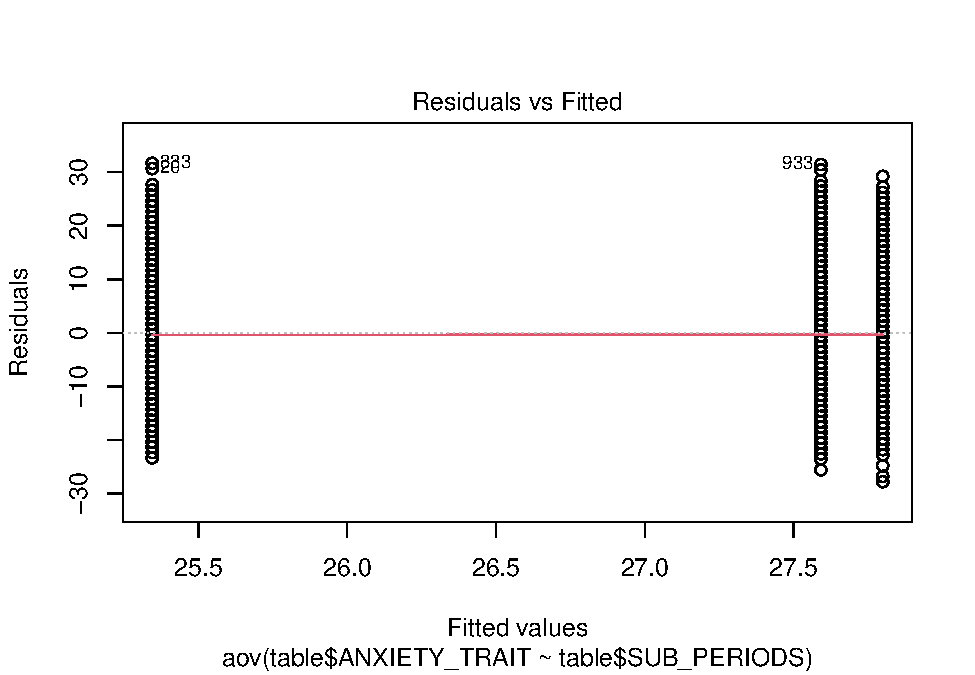
\includegraphics{Nexttry_files/figure-latex/unnamed-chunk-2-11.pdf} 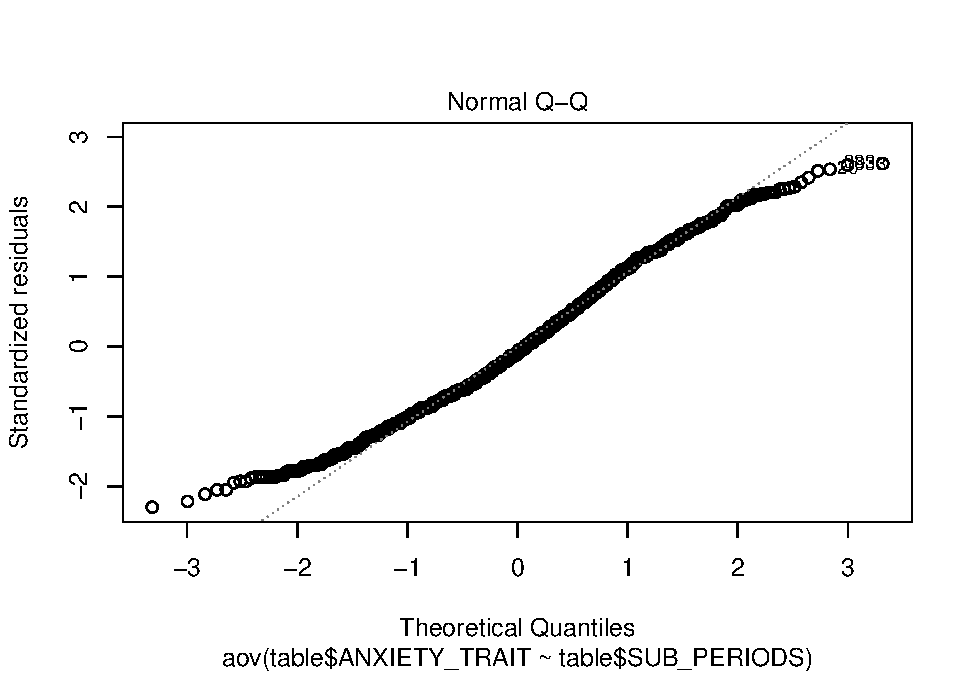
\includegraphics{Nexttry_files/figure-latex/unnamed-chunk-2-12.pdf} 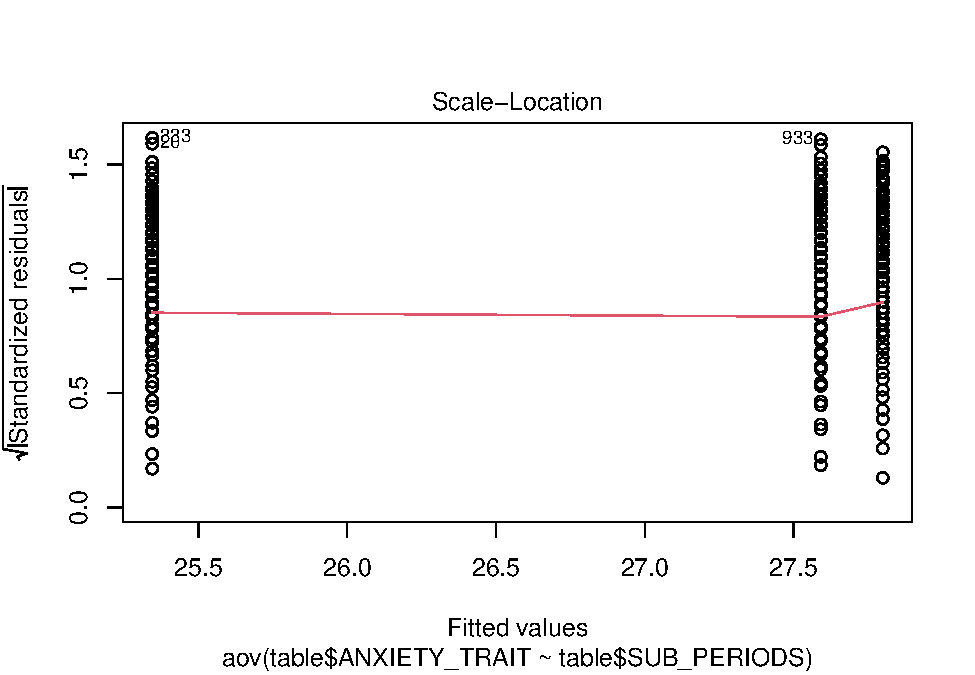
\includegraphics{Nexttry_files/figure-latex/unnamed-chunk-2-13.pdf} 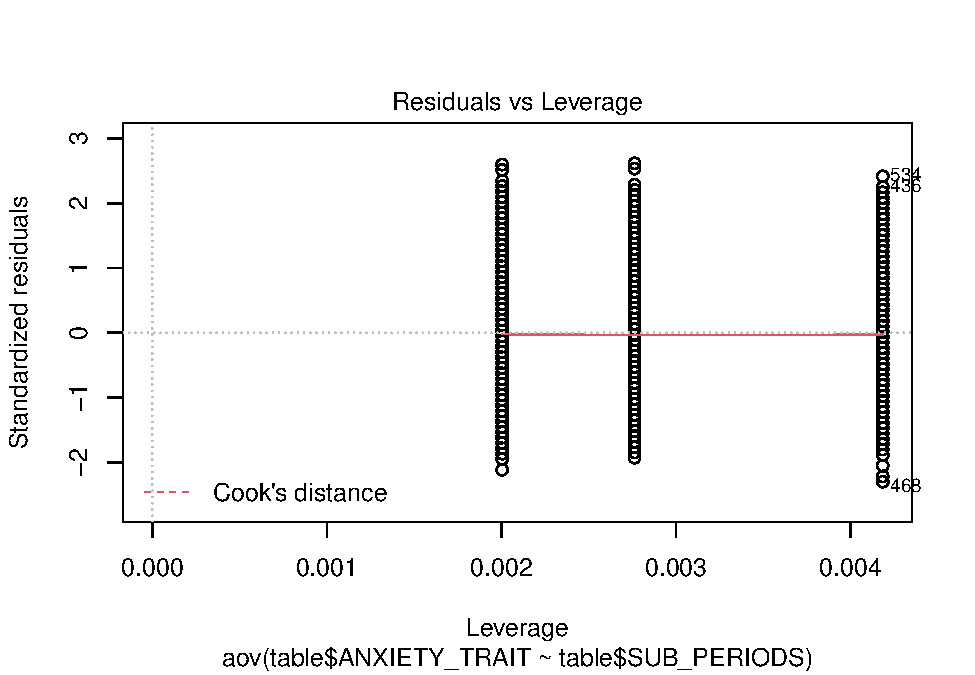
\includegraphics{Nexttry_files/figure-latex/unnamed-chunk-2-14.pdf}

\begin{Shaded}
\begin{Highlighting}[]
\FunctionTok{pairwise.t.test}\NormalTok{(}\AttributeTok{x =}\NormalTok{ table}\SpecialCharTok{$}\NormalTok{ANXIETY\_TRAIT, }\AttributeTok{g =}\NormalTok{ table}\SpecialCharTok{$}\NormalTok{SUB\_PERIODS, }\AttributeTok{p.adjust.method =} \StringTok{"bonferroni"}\NormalTok{, }\AttributeTok{pool.sd =} \ConstantTok{TRUE}\NormalTok{, }\AttributeTok{paired =} \ConstantTok{FALSE}\NormalTok{, }\AttributeTok{alternative =} \StringTok{"two.sided"}\NormalTok{)}
\end{Highlighting}
\end{Shaded}

\begin{verbatim}
## 
##  Pairwise comparisons using t tests with pooled SD 
## 
## data:  table$ANXIETY_TRAIT and table$SUB_PERIODS 
## 
##                1. EXT POST 2./3. EXT POST
## 2./3. EXT POST 0.046       -             
## 4. EXT POST    0.022       1.000         
## 
## P value adjustment method: bonferroni
\end{verbatim}

\begin{Shaded}
\begin{Highlighting}[]
\CommentTok{\# significant differences}
\CommentTok{\# 2./3. EXT POST{-}1. EXT POST p adj 0.046}
\CommentTok{\# 4. EXT POST{-}1. EXT POST p adj 0.022}
\CommentTok{\#effectsize::cohens\_f(anovatempanxtrait, ci = 0.95, partial = TRUE, type = 1)}

\FunctionTok{tapply}\NormalTok{(table}\SpecialCharTok{$}\NormalTok{ANXIETY\_TRAIT,}\FunctionTok{factor}\NormalTok{(table}\SpecialCharTok{$}\NormalTok{SUB\_PERIODS),mean)}
\end{Highlighting}
\end{Shaded}

\begin{verbatim}
##    1. EXT POST 2./3. EXT POST    4. EXT POST 
##       25.34530       27.79916       27.59118
\end{verbatim}

\begin{Shaded}
\begin{Highlighting}[]
\FunctionTok{tapply}\NormalTok{(table}\SpecialCharTok{$}\NormalTok{ANXIETY\_TRAIT,}\FunctionTok{factor}\NormalTok{(table}\SpecialCharTok{$}\NormalTok{SUB\_PERIODS),std.error)}
\end{Highlighting}
\end{Shaded}

\begin{verbatim}
##    1. EXT POST 2./3. EXT POST    4. EXT POST 
##      0.6266152      0.8316542      0.5315708
\end{verbatim}

\begin{Shaded}
\begin{Highlighting}[]
\CommentTok{\# Figure S3 (Supplementary material)}
\FunctionTok{plotmeans}\NormalTok{(table}\SpecialCharTok{$}\NormalTok{ANXIETY\_TRAIT}\SpecialCharTok{\textasciitilde{}}\NormalTok{table}\SpecialCharTok{$}\NormalTok{SUB\_PERIODS, }\AttributeTok{main=}\StringTok{"Fig. S3. Trait{-}Anxiety by quarantine sub{-}periods. Mean plot with 95\% Confidence Interval"}\NormalTok{, }\AttributeTok{cex.main =} \FloatTok{0.8}\NormalTok{, }\AttributeTok{ylab =} \StringTok{"Trait{-}Anxiety"}\NormalTok{, }\AttributeTok{xlab =} \StringTok{"Quarantine\textquotesingle{}s sub periods"}\NormalTok{)}
\end{Highlighting}
\end{Shaded}

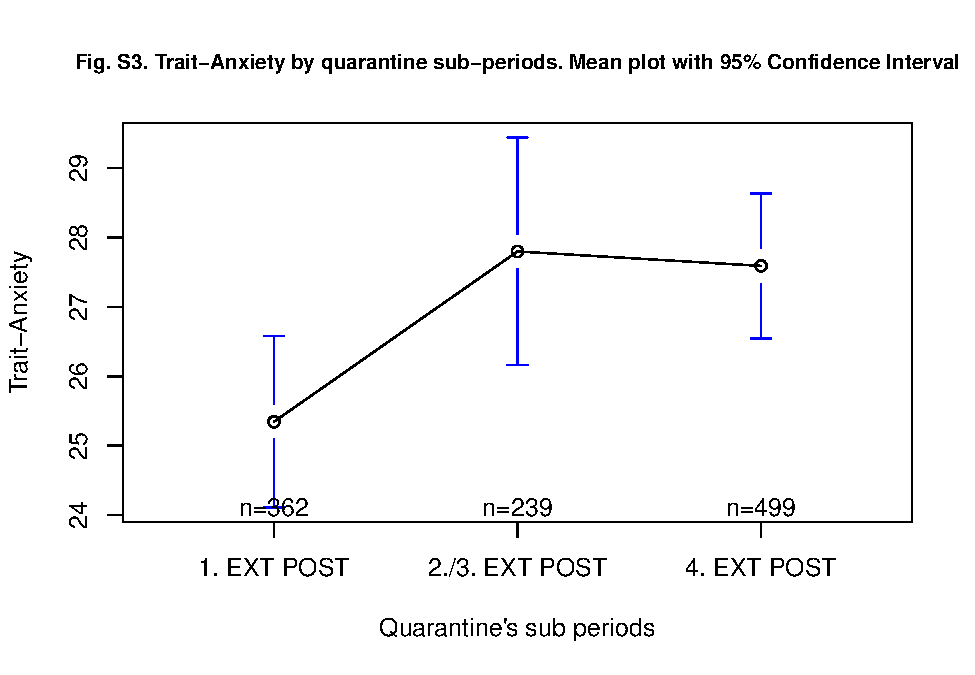
\includegraphics{Nexttry_files/figure-latex/unnamed-chunk-2-15.pdf}

\begin{Shaded}
\begin{Highlighting}[]
\FunctionTok{mean}\NormalTok{(table}\SpecialCharTok{$}\NormalTok{ANXIETY\_TRAIT) }\CommentTok{\# mean = 26.89727}
\end{Highlighting}
\end{Shaded}

\begin{verbatim}
## [1] 26.89727
\end{verbatim}

\begin{Shaded}
\begin{Highlighting}[]
\FunctionTok{std.error}\NormalTok{(table}\SpecialCharTok{$}\NormalTok{ANXIETY\_TRAIT) }\CommentTok{\# std. error = 0.3662711}
\end{Highlighting}
\end{Shaded}

\begin{verbatim}
## [1] 0.3662711
\end{verbatim}

\begin{Shaded}
\begin{Highlighting}[]
\CommentTok{\# low:}
\FunctionTok{prop.table}\NormalTok{(}\FunctionTok{table}\NormalTok{(table}\SpecialCharTok{$}\NormalTok{ANXIETY\_TRAIT}\SpecialCharTok{\textless{}}\DecValTok{27}\NormalTok{,table}\SpecialCharTok{$}\NormalTok{SUB\_PERIODS))}\SpecialCharTok{*}\DecValTok{100}
\end{Highlighting}
\end{Shaded}

\begin{verbatim}
##        
##         1. EXT POST 2./3. EXT POST 4. EXT POST
##   FALSE    14.54545       10.72727    22.63636
##   TRUE     18.36364       11.00000    22.72727
\end{verbatim}

\begin{Shaded}
\begin{Highlighting}[]
\CommentTok{\# high:}
\FunctionTok{prop.table}\NormalTok{(}\FunctionTok{table}\NormalTok{(table}\SpecialCharTok{$}\NormalTok{ANXIETY\_TRAIT}\SpecialCharTok{\textgreater{}=}\DecValTok{27}\NormalTok{,table}\SpecialCharTok{$}\NormalTok{SUB\_PERIODS))}\SpecialCharTok{*}\DecValTok{100}
\end{Highlighting}
\end{Shaded}

\begin{verbatim}
##        
##         1. EXT POST 2./3. EXT POST 4. EXT POST
##   FALSE    18.36364       11.00000    22.72727
##   TRUE     14.54545       10.72727    22.63636
\end{verbatim}

\begin{Shaded}
\begin{Highlighting}[]
\CommentTok{\# SUICIDAL RISK}
\NormalTok{anovatempsuic }\OtherTok{\textless{}{-}} \FunctionTok{aov}\NormalTok{(table}\SpecialCharTok{$}\NormalTok{SUIC\_RISK}\SpecialCharTok{\textasciitilde{}}\NormalTok{table}\SpecialCharTok{$}\NormalTok{SUB\_PERIODS)}
\NormalTok{anovatempsuic}
\end{Highlighting}
\end{Shaded}

\begin{verbatim}
## Call:
##    aov(formula = table$SUIC_RISK ~ table$SUB_PERIODS)
## 
## Terms:
##                 table$SUB_PERIODS Residuals
## Sum of Squares            2143.68 291314.40
## Deg. of Freedom                 2      1097
## 
## Residual standard error: 16.29587
## Estimated effects may be unbalanced
\end{verbatim}

\begin{Shaded}
\begin{Highlighting}[]
\FunctionTok{summary}\NormalTok{(anovatempsuic)}
\end{Highlighting}
\end{Shaded}

\begin{verbatim}
##                     Df Sum Sq Mean Sq F value Pr(>F)  
## table$SUB_PERIODS    2   2144  1071.8   4.036 0.0179 *
## Residuals         1097 291314   265.6                 
## ---
## Signif. codes:  0 '***' 0.001 '**' 0.01 '*' 0.05 '.' 0.1 ' ' 1
\end{verbatim}

\begin{Shaded}
\begin{Highlighting}[]
\FunctionTok{plot}\NormalTok{(anovatempsuic)}
\end{Highlighting}
\end{Shaded}

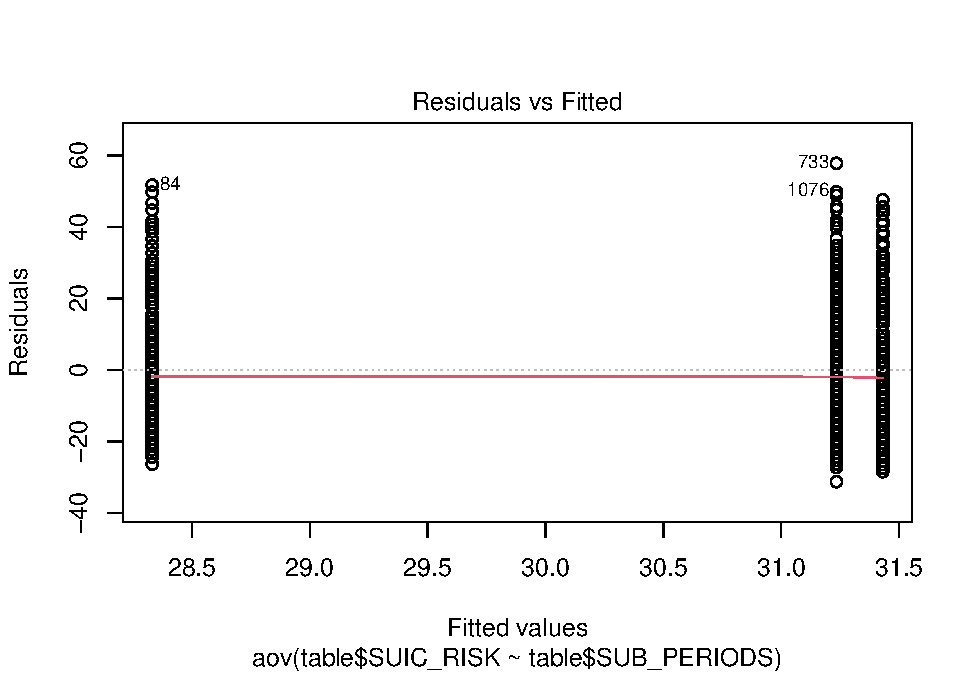
\includegraphics{Nexttry_files/figure-latex/unnamed-chunk-2-16.pdf} 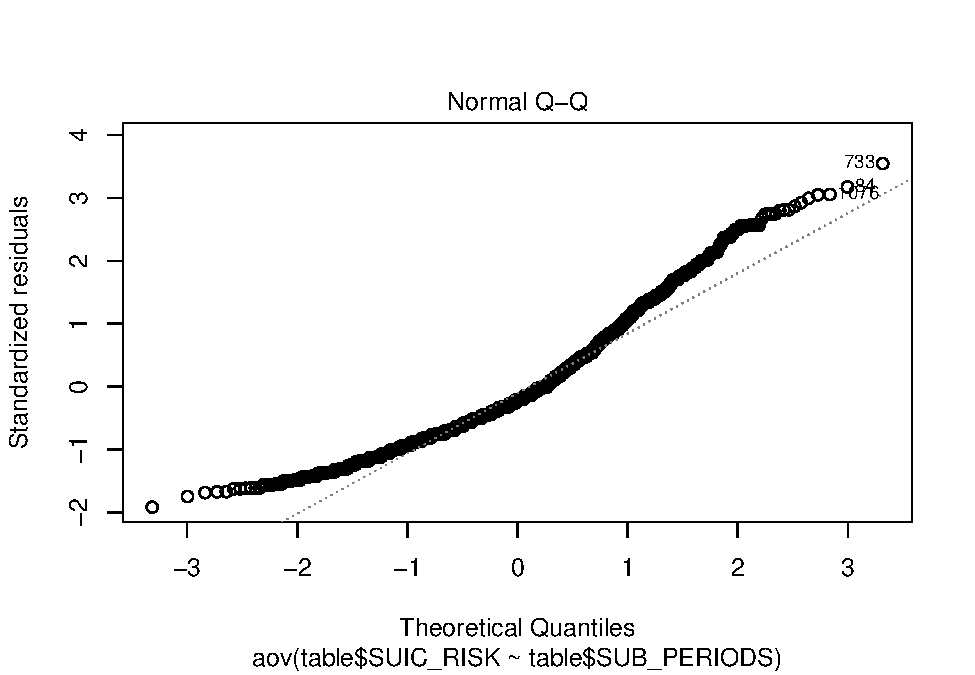
\includegraphics{Nexttry_files/figure-latex/unnamed-chunk-2-17.pdf} 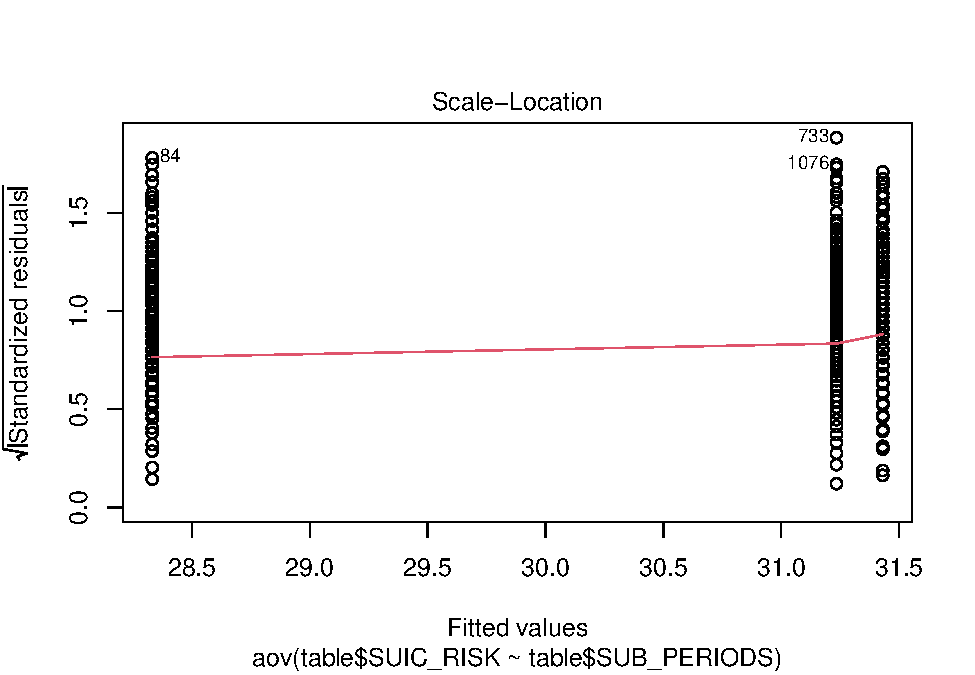
\includegraphics{Nexttry_files/figure-latex/unnamed-chunk-2-18.pdf} 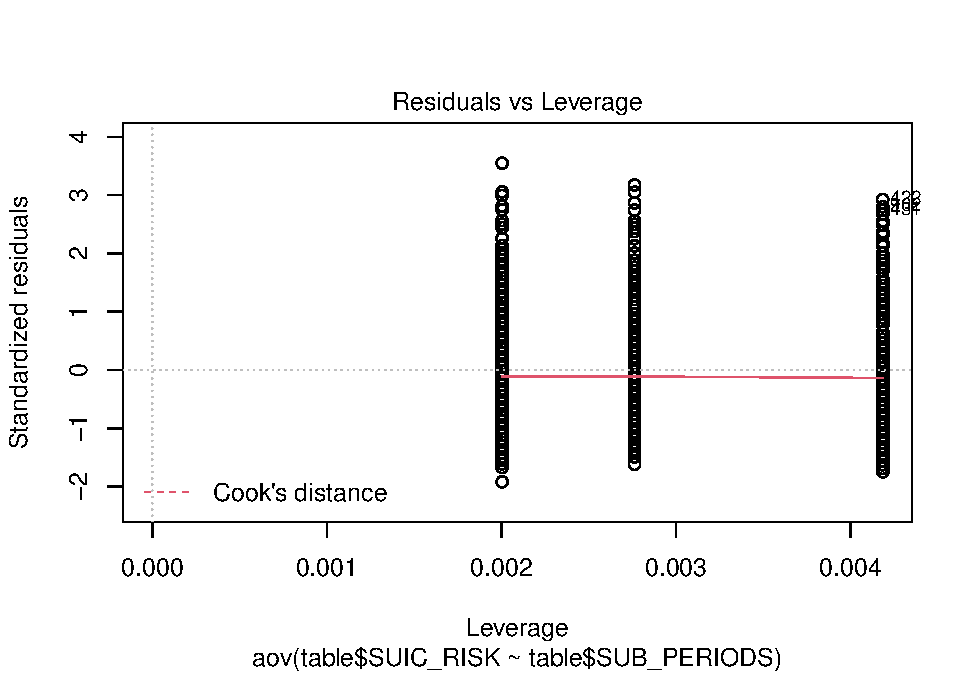
\includegraphics{Nexttry_files/figure-latex/unnamed-chunk-2-19.pdf}

\begin{Shaded}
\begin{Highlighting}[]
\FunctionTok{pairwise.t.test}\NormalTok{(}\AttributeTok{x =}\NormalTok{ table}\SpecialCharTok{$}\NormalTok{SUIC\_RISK, }\AttributeTok{g =}\NormalTok{ table}\SpecialCharTok{$}\NormalTok{SUB\_PERIODS, }\AttributeTok{p.adjust.method =} \StringTok{"bonferroni"}\NormalTok{, }\AttributeTok{pool.sd =} \ConstantTok{TRUE}\NormalTok{, }\AttributeTok{paired =} \ConstantTok{FALSE}\NormalTok{, }\AttributeTok{alternative =} \StringTok{"two.sided"}\NormalTok{)}
\end{Highlighting}
\end{Shaded}

\begin{verbatim}
## 
##  Pairwise comparisons using t tests with pooled SD 
## 
## data:  table$SUIC_RISK and table$SUB_PERIODS 
## 
##                1. EXT POST 2./3. EXT POST
## 2./3. EXT POST 0.068       -             
## 4. EXT POST    0.030       1.000         
## 
## P value adjustment method: bonferroni
\end{verbatim}

\begin{Shaded}
\begin{Highlighting}[]
\CommentTok{\# significant differences}
\CommentTok{\# 4. EXT POST{-}1. EXT POST p adj 0.030}
\CommentTok{\#effectsize::cohens\_f(anovatempsuic, ci = 0.95, partial = TRUE, type = 1)}

\FunctionTok{tapply}\NormalTok{(table}\SpecialCharTok{$}\NormalTok{SUIC\_RISK,}\FunctionTok{factor}\NormalTok{(table}\SpecialCharTok{$}\NormalTok{SUB\_PERIODS),mean)}
\end{Highlighting}
\end{Shaded}

\begin{verbatim}
##    1. EXT POST 2./3. EXT POST    4. EXT POST 
##       28.33149       31.43096       31.23447
\end{verbatim}

\begin{Shaded}
\begin{Highlighting}[]
\FunctionTok{tapply}\NormalTok{(table}\SpecialCharTok{$}\NormalTok{SUIC\_RISK,}\FunctionTok{factor}\NormalTok{(table}\SpecialCharTok{$}\NormalTok{SUB\_PERIODS),std.error)}
\end{Highlighting}
\end{Shaded}

\begin{verbatim}
##    1. EXT POST 2./3. EXT POST    4. EXT POST 
##      0.7902982      1.1492061      0.7358880
\end{verbatim}

\begin{Shaded}
\begin{Highlighting}[]
\CommentTok{\# Figure S4 (Supplementary material)}
\FunctionTok{plotmeans}\NormalTok{(table}\SpecialCharTok{$}\NormalTok{SUIC\_RISK}\SpecialCharTok{\textasciitilde{}}\NormalTok{table}\SpecialCharTok{$}\NormalTok{SUB\_PERIODS, }\AttributeTok{main=}\StringTok{"Fig. S4. Suicidal risk by quarantine sub{-}periods. Mean plot with 95\% Confidence Interval"}\NormalTok{, }\AttributeTok{cex.main =} \FloatTok{0.8}\NormalTok{, }\AttributeTok{ylab =} \StringTok{"Suicidal risk"}\NormalTok{, }\AttributeTok{xlab =} \StringTok{"Quarantine\textquotesingle{}s sub periods"}\NormalTok{)}
\end{Highlighting}
\end{Shaded}

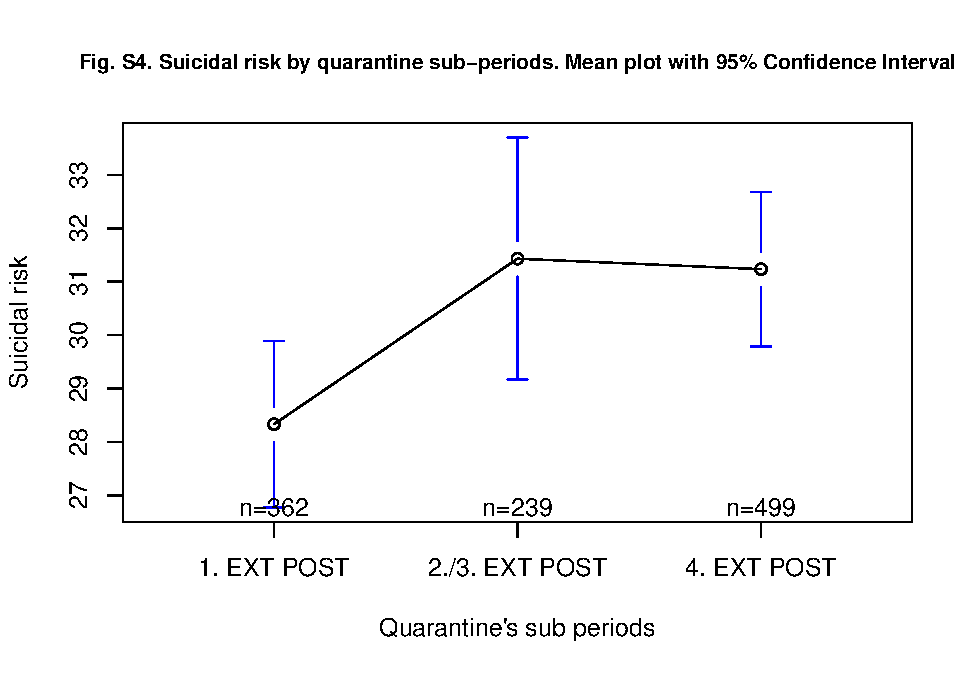
\includegraphics{Nexttry_files/figure-latex/unnamed-chunk-2-20.pdf}

\begin{Shaded}
\begin{Highlighting}[]
\FunctionTok{mean}\NormalTok{(table}\SpecialCharTok{$}\NormalTok{SUIC\_RISK) }\CommentTok{\# mean = 30.32182}
\end{Highlighting}
\end{Shaded}

\begin{verbatim}
## [1] 30.32182
\end{verbatim}

\begin{Shaded}
\begin{Highlighting}[]
\FunctionTok{std.error}\NormalTok{(table}\SpecialCharTok{$}\NormalTok{SUIC\_RISK) }\CommentTok{\# std. error = 0.4926946}
\end{Highlighting}
\end{Shaded}

\begin{verbatim}
## [1] 0.4926946
\end{verbatim}

\begin{Shaded}
\begin{Highlighting}[]
\CommentTok{\# Percentage distribution by cutoff score:}
\CommentTok{\# low:}
\FunctionTok{prop.table}\NormalTok{(}\FunctionTok{table}\NormalTok{(table}\SpecialCharTok{$}\NormalTok{SUIC\_RISK}\SpecialCharTok{\textless{}}\DecValTok{30}\NormalTok{,table}\SpecialCharTok{$}\NormalTok{SUB\_PERIODS))}\SpecialCharTok{*}\DecValTok{100}
\end{Highlighting}
\end{Shaded}

\begin{verbatim}
##        
##         1. EXT POST 2./3. EXT POST 4. EXT POST
##   FALSE   12.181818       9.909091   20.181818
##   TRUE    20.727273      11.818182   25.181818
\end{verbatim}

\begin{Shaded}
\begin{Highlighting}[]
\CommentTok{\# moderate:}
\FunctionTok{prop.table}\NormalTok{(}\FunctionTok{table}\NormalTok{(table}\SpecialCharTok{$}\NormalTok{SUIC\_RISK}\SpecialCharTok{\textgreater{}=}\DecValTok{30}\SpecialCharTok{\&}\NormalTok{table}\SpecialCharTok{$}\NormalTok{SUIC\_RISK}\SpecialCharTok{\textless{}=}\DecValTok{44}\NormalTok{,table}\SpecialCharTok{$}\NormalTok{SUB\_PERIODS))}\SpecialCharTok{*}\DecValTok{100}
\end{Highlighting}
\end{Shaded}

\begin{verbatim}
##        
##         1. EXT POST 2./3. EXT POST 4. EXT POST
##   FALSE   25.090909      16.727273   35.272727
##   TRUE     7.818182       5.000000   10.090909
\end{verbatim}

\begin{Shaded}
\begin{Highlighting}[]
\CommentTok{\# high:}
\FunctionTok{prop.table}\NormalTok{(}\FunctionTok{table}\NormalTok{(table}\SpecialCharTok{$}\NormalTok{SUIC\_RISK}\SpecialCharTok{\textgreater{}=}\DecValTok{45}\NormalTok{,table}\SpecialCharTok{$}\NormalTok{SUB\_PERIODS))}\SpecialCharTok{*}\DecValTok{100}
\end{Highlighting}
\end{Shaded}

\begin{verbatim}
##        
##         1. EXT POST 2./3. EXT POST 4. EXT POST
##   FALSE   28.545455      16.818182   35.272727
##   TRUE     4.363636       4.909091   10.090909
\end{verbatim}

\begin{Shaded}
\begin{Highlighting}[]
\DocumentationTok{\#\#\#\#\#\#\#\#\#\#\#\#\#\#\#\#\#\#\#\#\#\#\#\#\#\#\#\#\#\#\#\#\#\#\#\#\#\#\#\#\#\#\#\#\#\#\#\#\#\#\#\#\#\#\#\#\#\#\#\#\#\#\#\#\#\#\#\#\#\#\#\#\#\#\#\#\#\#\#\#\#\#\#\#\#\#\#\#\#\#\#}
\DocumentationTok{\#\#\#\#\#\#\#\#\#\#\#\#\#\#\#\#\#\#\#\#\#\#\#\#\#\#\#\#\#\#\#\#\#\#\#\#\#\#\#\#\# AIM 2 \#\#\#\#\#\#\#\#\#\#\#\#\#\#\#\#\#\#\#\#\#\#\#\#\#\#\#\#\#\#\#\#\#\#\#\#\#\#\#\#\#\#\#}

\DocumentationTok{\#\#\#\#\#\#\#\#\#\#\#\#\#\#\#\#\#\#\#\#\#\#\#\#\#\#\#\#\#\#\#\#\#\#\#\#\#\#\#\#\#\#\#\#\#\#\#\#\#\#\#\#\#\#\#\#\#\#\#\#\#\#\#\#\#\#\#\#\#\#\#\#\#\#}
\DocumentationTok{\#\# 2) Multiple linear regressions:}

\CommentTok{\# We performed stepwise selection (direction = both) using the stepAIC() function from the MASS package.}
\FunctionTok{library}\NormalTok{(MASS)}
\end{Highlighting}
\end{Shaded}

\begin{verbatim}
## 
## Attaching package: 'MASS'
\end{verbatim}

\begin{verbatim}
## The following object is masked from 'package:dplyr':
## 
##     select
\end{verbatim}

\begin{Shaded}
\begin{Highlighting}[]
\CommentTok{\# stepAIC() performs stepwise model selection by exact AIC}


\DocumentationTok{\#\#\#\# DEPRESSION:}
\CommentTok{\# Stepwise Regression}
\NormalTok{fitwith}\OtherTok{\textless{}{-}}\FunctionTok{lm}\NormalTok{(DEPRESSION}\SpecialCharTok{\textasciitilde{}}\NormalTok{SEX}\SpecialCharTok{+}\NormalTok{AGE}\SpecialCharTok{+}\NormalTok{PROVINCE}\SpecialCharTok{+}\NormalTok{EDUCATION}\SpecialCharTok{+}\NormalTok{ECONOMIC\_INCOME}\SpecialCharTok{+}\NormalTok{LIVING\_WITH\_SOMEBODY}\SpecialCharTok{+}\NormalTok{MENTAL\_DISORDER\_HISTORY}\SpecialCharTok{+}\NormalTok{SUIC\_ATTEMPT\_HISTORY}\SpecialCharTok{+}\NormalTok{SUB\_PERIODS,}\AttributeTok{data=}\NormalTok{table)}
\NormalTok{stepwith }\OtherTok{\textless{}{-}} \FunctionTok{stepAIC}\NormalTok{(fitwith, }\AttributeTok{trace=}\ConstantTok{TRUE}\NormalTok{,}\AttributeTok{direction=}\StringTok{"both"}\NormalTok{)}
\end{Highlighting}
\end{Shaded}

\begin{verbatim}
## Start:  AIC=4951.51
## DEPRESSION ~ SEX + AGE + PROVINCE + EDUCATION + ECONOMIC_INCOME + 
##     LIVING_WITH_SOMEBODY + MENTAL_DISORDER_HISTORY + SUIC_ATTEMPT_HISTORY + 
##     SUB_PERIODS
## 
##                           Df Sum of Sq    RSS    AIC
## - PROVINCE                25    3682.6  95380 4944.8
## - EDUCATION                8    1052.2  92750 4948.1
## - LIVING_WITH_SOMEBODY     1       3.5  91701 4949.5
## <none>                                  91698 4951.5
## - ECONOMIC_INCOME          1     175.8  91874 4951.6
## - SUB_PERIODS              2     735.9  92434 4956.3
## - MENTAL_DISORDER_HISTORY  1    1336.6  93034 4965.4
## - SEX                      1    2274.4  93972 4976.5
## - AGE                      1    4345.7  96044 5000.4
## - SUIC_ATTEMPT_HISTORY     2   11683.5 103381 5079.4
## 
## Step:  AIC=4944.82
## DEPRESSION ~ SEX + AGE + EDUCATION + ECONOMIC_INCOME + LIVING_WITH_SOMEBODY + 
##     MENTAL_DISORDER_HISTORY + SUIC_ATTEMPT_HISTORY + SUB_PERIODS
## 
##                           Df Sum of Sq    RSS    AIC
## - EDUCATION                8    1030.5  96411 4940.6
## - LIVING_WITH_SOMEBODY     1       2.8  95383 4942.9
## <none>                                  95380 4944.8
## - ECONOMIC_INCOME          1     240.6  95621 4945.6
## + PROVINCE                25    3682.6  91698 4951.5
## - SUB_PERIODS              2    1041.4  96422 4952.8
## - MENTAL_DISORDER_HISTORY  1    1350.0  96730 4958.3
## - SEX                      1    2549.9  97930 4971.8
## - AGE                      1    4686.4 100067 4995.6
## - SUIC_ATTEMPT_HISTORY     2   12809.5 108190 5079.4
## 
## Step:  AIC=4940.64
## DEPRESSION ~ SEX + AGE + ECONOMIC_INCOME + LIVING_WITH_SOMEBODY + 
##     MENTAL_DISORDER_HISTORY + SUIC_ATTEMPT_HISTORY + SUB_PERIODS
## 
##                           Df Sum of Sq    RSS    AIC
## - LIVING_WITH_SOMEBODY     1       5.3  96416 4938.7
## <none>                                  96411 4940.6
## - ECONOMIC_INCOME          1     368.1  96779 4942.8
## + EDUCATION                8    1030.5  95380 4944.8
## + PROVINCE                25    3660.8  92750 4948.1
## - SUB_PERIODS              2    1067.3  97478 4948.7
## - MENTAL_DISORDER_HISTORY  1    1246.3  97657 4952.8
## - SEX                      1    2578.1  98989 4967.7
## - AGE                      1    6060.8 102472 5005.7
## - SUIC_ATTEMPT_HISTORY     2   13690.6 110101 5082.7
## 
## Step:  AIC=4938.7
## DEPRESSION ~ SEX + AGE + ECONOMIC_INCOME + MENTAL_DISORDER_HISTORY + 
##     SUIC_ATTEMPT_HISTORY + SUB_PERIODS
## 
##                           Df Sum of Sq    RSS    AIC
## <none>                                  96416 4938.7
## + LIVING_WITH_SOMEBODY     1       5.3  96411 4940.6
## - ECONOMIC_INCOME          1     375.1  96791 4941.0
## + EDUCATION                8    1033.0  95383 4942.9
## + PROVINCE                25    3660.4  92756 4946.1
## - SUB_PERIODS              2    1069.1  97485 4946.8
## - MENTAL_DISORDER_HISTORY  1    1241.0  97657 4950.8
## - SEX                      1    2606.6  99023 4966.0
## - AGE                      1    6225.6 102642 5005.5
## - SUIC_ATTEMPT_HISTORY     2   13688.5 110105 5080.7
\end{verbatim}

\begin{Shaded}
\begin{Highlighting}[]
\NormalTok{stepwith}
\end{Highlighting}
\end{Shaded}

\begin{verbatim}
## 
## Call:
## lm(formula = DEPRESSION ~ SEX + AGE + ECONOMIC_INCOME + MENTAL_DISORDER_HISTORY + 
##     SUIC_ATTEMPT_HISTORY + SUB_PERIODS, data = table)
## 
## Coefficients:
##                (Intercept)                    SEXwoman  
##                    22.8913                      3.9272  
##                        AGE          ECONOMIC_INCOMEyes  
##                    -0.2182                     -1.6117  
## MENTAL_DISORDER_HISTORYyes      SUIC_ATTEMPT_HISTORYno  
##                     2.5083                     -6.7037  
##    SUIC_ATTEMPT_HISTORYyes   SUB_PERIODS2./3. EXT POST  
##                     4.8715                      1.5511  
##     SUB_PERIODS4. EXT POST  
##                     2.3125
\end{verbatim}

\begin{Shaded}
\begin{Highlighting}[]
\NormalTok{stepwith}\SpecialCharTok{$}\NormalTok{anova }\CommentTok{\# display results}
\end{Highlighting}
\end{Shaded}

\begin{verbatim}
## Stepwise Model Path 
## Analysis of Deviance Table
## 
## Initial Model:
## DEPRESSION ~ SEX + AGE + PROVINCE + EDUCATION + ECONOMIC_INCOME + 
##     LIVING_WITH_SOMEBODY + MENTAL_DISORDER_HISTORY + SUIC_ATTEMPT_HISTORY + 
##     SUB_PERIODS
## 
## Final Model:
## DEPRESSION ~ SEX + AGE + ECONOMIC_INCOME + MENTAL_DISORDER_HISTORY + 
##     SUIC_ATTEMPT_HISTORY + SUB_PERIODS
## 
## 
##                     Step Df    Deviance Resid. Df Resid. Dev      AIC
## 1                                            1057   91697.83 4951.507
## 2             - PROVINCE 25 3682.560562      1082   95380.39 4944.819
## 3            - EDUCATION  8 1030.467448      1090   96410.86 4940.640
## 4 - LIVING_WITH_SOMEBODY  1    5.331578      1091   96416.19 4938.700
\end{verbatim}

\begin{Shaded}
\begin{Highlighting}[]
\CommentTok{\# Stepwise Model Path }
\CommentTok{\# Analysis of Deviance Table}
\CommentTok{\# Initial Model: DEPRESSION \textasciitilde{} SEX + AGE + PROVINCE + EDUCATION + ECONOMIC\_INCOME + LIVING\_WITH\_SOMEBODY + MENTAL\_DISORDER\_HISTORY + SUIC\_ATTEMPT\_HISTORY + SUB\_PERIODS}
\CommentTok{\# Start:  AIC = 4951.51}
\CommentTok{\# Final Model: DEPRESSION \textasciitilde{} SEX + AGE + ECONOMIC\_INCOME + MENTAL\_DISORDER\_HISTORY + SUIC\_ATTEMPT\_HISTORY + SUB\_PERIODS}
\CommentTok{\# Stepwith:  AIC = 4938.7}
\FunctionTok{summary}\NormalTok{(stepwith)}
\end{Highlighting}
\end{Shaded}

\begin{verbatim}
## 
## Call:
## lm(formula = DEPRESSION ~ SEX + AGE + ECONOMIC_INCOME + MENTAL_DISORDER_HISTORY + 
##     SUIC_ATTEMPT_HISTORY + SUB_PERIODS, data = table)
## 
## Residuals:
##     Min      1Q  Median      3Q     Max 
## -25.519  -6.393  -1.064   5.114  34.131 
## 
## Coefficients:
##                            Estimate Std. Error t value Pr(>|t|)    
## (Intercept)                 22.8913     1.3652  16.768  < 2e-16 ***
## SEXwoman                     3.9272     0.7231   5.431 6.91e-08 ***
## AGE                         -0.2182     0.0260  -8.393  < 2e-16 ***
## ECONOMIC_INCOMEyes          -1.6117     0.7823  -2.060 0.039627 *  
## MENTAL_DISORDER_HISTORYyes   2.5083     0.6694   3.747 0.000188 ***
## SUIC_ATTEMPT_HISTORYno      -6.7037     0.6863  -9.767  < 2e-16 ***
## SUIC_ATTEMPT_HISTORYyes      4.8715     1.2486   3.901 0.000101 ***
## SUB_PERIODS2./3. EXT POST    1.5511     0.7854   1.975 0.048546 *  
## SUB_PERIODS4. EXT POST       2.3125     0.6697   3.453 0.000575 ***
## ---
## Signif. codes:  0 '***' 0.001 '**' 0.01 '*' 0.05 '.' 0.1 ' ' 1
## 
## Residual standard error: 9.401 on 1091 degrees of freedom
## Multiple R-squared:  0.2881, Adjusted R-squared:  0.2829 
## F-statistic: 55.19 on 8 and 1091 DF,  p-value: < 2.2e-16
\end{verbatim}

\begin{Shaded}
\begin{Highlighting}[]
\CommentTok{\# 95\% Confidence interval of best{-}fitted model:}
\FunctionTok{confint}\NormalTok{(stepwith)}
\end{Highlighting}
\end{Shaded}

\begin{verbatim}
##                                   2.5 %      97.5 %
## (Intercept)                20.212619617 25.56999549
## SEXwoman                    2.508307273  5.34600026
## AGE                        -0.269236094 -0.16720616
## ECONOMIC_INCOMEyes         -3.146793263 -0.07662992
## MENTAL_DISORDER_HISTORYyes  1.194942661  3.82165836
## SUIC_ATTEMPT_HISTORYno     -8.050428044 -5.35705695
## SUIC_ATTEMPT_HISTORYyes     2.421494846  7.32143786
## SUB_PERIODS2./3. EXT POST   0.009920813  3.09221838
## SUB_PERIODS4. EXT POST      0.998527485  3.62653957
\end{verbatim}

\begin{Shaded}
\begin{Highlighting}[]
\CommentTok{\# ERROR RATE of best{-}fitted model:}
\FunctionTok{sigma}\NormalTok{(stepwith)}\SpecialCharTok{/}\FunctionTok{mean}\NormalTok{(table}\SpecialCharTok{$}\NormalTok{DEPRESSION)}
\end{Highlighting}
\end{Shaded}

\begin{verbatim}
## [1] 0.5989474
\end{verbatim}

\begin{Shaded}
\begin{Highlighting}[]
\CommentTok{\# 0.5989474}
\CommentTok{\# In our multiple regression example, the Residual Standard Error (RSE) or sigma is 9.401 corresponding to 60\% error rate.}

\FunctionTok{par}\NormalTok{(}\AttributeTok{mfrow=}\FunctionTok{c}\NormalTok{(}\DecValTok{2}\NormalTok{,}\DecValTok{2}\NormalTok{))}
\CommentTok{\# Figure S5 (Supplementary material)}
\FunctionTok{plot}\NormalTok{(stepwith)}
\end{Highlighting}
\end{Shaded}

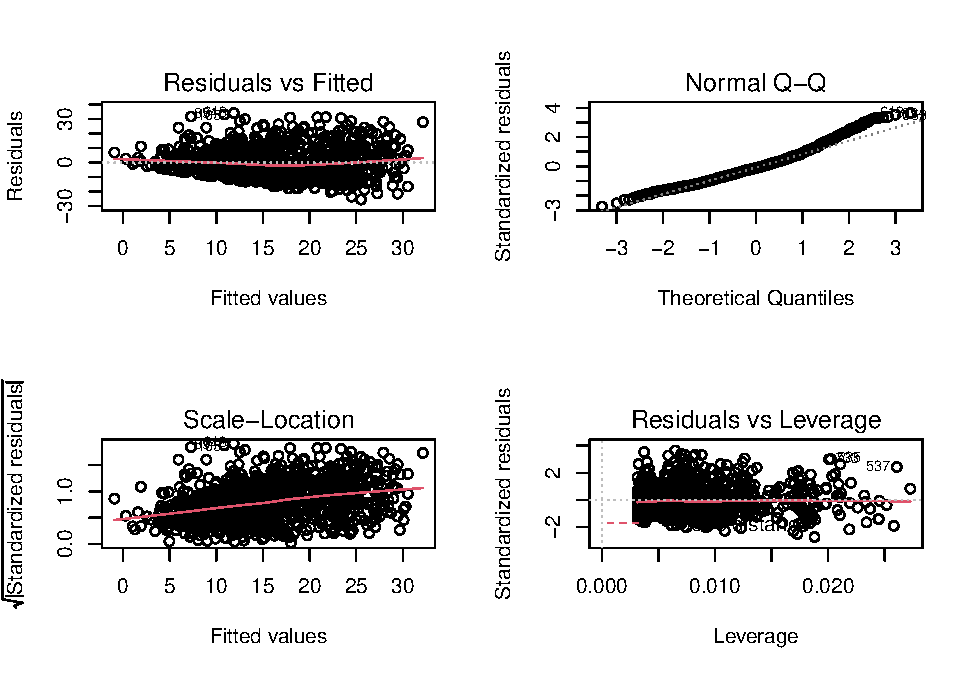
\includegraphics{Nexttry_files/figure-latex/unnamed-chunk-2-21.pdf}

\begin{Shaded}
\begin{Highlighting}[]
\FunctionTok{par}\NormalTok{(}\AttributeTok{mfrow=}\FunctionTok{c}\NormalTok{(}\DecValTok{1}\NormalTok{,}\DecValTok{1}\NormalTok{))}


\CommentTok{\# TABLE 1:}

\CommentTok{\# Model 1: INITIAL MODEL:}
\NormalTok{model1}\OtherTok{\textless{}{-}}\FunctionTok{lm}\NormalTok{(DEPRESSION}\SpecialCharTok{\textasciitilde{}}\NormalTok{SEX}\SpecialCharTok{+}\NormalTok{AGE}\SpecialCharTok{+}\NormalTok{PROVINCE}\SpecialCharTok{+}\NormalTok{EDUCATION}\SpecialCharTok{+}\NormalTok{ECONOMIC\_INCOME}\SpecialCharTok{+}\NormalTok{LIVING\_WITH\_SOMEBODY}\SpecialCharTok{+}\NormalTok{MENTAL\_DISORDER\_HISTORY}\SpecialCharTok{+}\NormalTok{SUIC\_ATTEMPT\_HISTORY}\SpecialCharTok{+}\NormalTok{SUB\_PERIODS,}\AttributeTok{data=}\NormalTok{table)}
\FunctionTok{summary}\NormalTok{(model1)}
\end{Highlighting}
\end{Shaded}

\begin{verbatim}
## 
## Call:
## lm(formula = DEPRESSION ~ SEX + AGE + PROVINCE + EDUCATION + 
##     ECONOMIC_INCOME + LIVING_WITH_SOMEBODY + MENTAL_DISORDER_HISTORY + 
##     SUIC_ATTEMPT_HISTORY + SUB_PERIODS, data = table)
## 
## Residuals:
##     Min      1Q  Median      3Q     Max 
## -23.839  -6.235  -0.880   4.810  34.667 
## 
## Coefficients:
##                                            Estimate Std. Error t value Pr(>|t|)
## (Intercept)                                 14.1136     6.8720   2.054 0.040240
## SEXwoman                                     3.7600     0.7343   5.120 3.62e-07
## AGE                                         -0.2039     0.0288  -7.078 2.67e-12
## PROVINCECABA (Buenos Aires capital)         -2.6299     1.1436  -2.300 0.021657
## PROVINCECatamarca                            1.5213     6.7415   0.226 0.821511
## PROVINCEChaco                               -3.8453     3.6088  -1.066 0.286876
## PROVINCEChubut                              -1.6699     4.7235  -0.354 0.723763
## PROVINCECórdoba                             -3.0918     0.8848  -3.494 0.000495
## PROVINCECorrientes                          -5.8987     4.2371  -1.392 0.164166
## PROVINCEEntre Ríos                           1.3188     2.5256   0.522 0.601647
## PROVINCEFormosa                              7.0780     5.4450   1.300 0.193917
## PROVINCEJujuy                               -0.9570     1.7410  -0.550 0.582650
## PROVINCELa Pampa                            -6.2685     3.3805  -1.854 0.063971
## PROVINCELa Rioja                            -9.1692     9.4036  -0.975 0.329747
## PROVINCEMendoza                             -0.2200     2.3827  -0.092 0.926459
## PROVINCEMisiones                            -4.5683     2.5899  -1.764 0.078037
## PROVINCENeuquén                             -6.3639     3.2784  -1.941 0.052503
## PROVINCEother                               -2.4944     2.3334  -1.069 0.285317
## PROVINCEOtro                                -0.7964     5.4997  -0.145 0.884893
## PROVINCERío Negro                            2.8514     4.7250   0.603 0.546328
## PROVINCESalta                                5.1110     2.7891   1.832 0.067160
## PROVINCESan Juan                             0.3405     4.7553   0.072 0.942924
## PROVINCESan Luis                            19.3126     9.3942   2.056 0.040048
## PROVINCESanta Cruz                           3.8887     6.6448   0.585 0.558517
## PROVINCESanta Fe                            -2.7375     0.8800  -3.111 0.001915
## PROVINCESantiago del Estero                 -1.4102     2.5911  -0.544 0.586396
## PROVINCETierra del Fuego                    -2.4344     2.2629  -1.076 0.282261
## PROVINCETucumán                             -1.9335     1.9762  -0.978 0.328093
## EDUCATIONCompleted high school              10.7046     6.7151   1.594 0.111212
## EDUCATIONCompleted postgraduate              8.5487     6.7144   1.273 0.203229
## EDUCATIONCompleted tertiary or university    9.4013     6.6823   1.407 0.159755
## EDUCATIONIncomplete elementary school        9.1756    11.4762   0.800 0.424159
## EDUCATIONIncomplete high school             14.5440     6.9355   2.097 0.036227
## EDUCATIONIncomplete postgraduate             9.7746     6.7411   1.450 0.147353
## EDUCATIONIncomplete tertiary or university   9.6203     6.6747   1.441 0.149797
## EDUCATIONOtro                               16.0206     9.5233   1.682 0.092816
## ECONOMIC_INCOMEyes                          -1.1366     0.7984  -1.424 0.154874
## LIVING_WITH_SOMEBODYyes                      0.1651     0.8268   0.200 0.841778
## MENTAL_DISORDER_HISTORYyes                   2.6463     0.6742   3.925 9.23e-05
## SUIC_ATTEMPT_HISTORYno                      -6.2399     0.6963  -8.962  < 2e-16
## SUIC_ATTEMPT_HISTORYyes                      4.9458     1.2525   3.949 8.37e-05
## SUB_PERIODS2./3. EXT POST                    1.1705     0.8316   1.408 0.159570
## SUB_PERIODS4. EXT POST                       2.2370     0.7682   2.912 0.003666
##                                               
## (Intercept)                                *  
## SEXwoman                                   ***
## AGE                                        ***
## PROVINCECABA (Buenos Aires capital)        *  
## PROVINCECatamarca                             
## PROVINCEChaco                                 
## PROVINCEChubut                                
## PROVINCECórdoba                            ***
## PROVINCECorrientes                            
## PROVINCEEntre Ríos                            
## PROVINCEFormosa                               
## PROVINCEJujuy                                 
## PROVINCELa Pampa                           .  
## PROVINCELa Rioja                              
## PROVINCEMendoza                               
## PROVINCEMisiones                           .  
## PROVINCENeuquén                            .  
## PROVINCEother                                 
## PROVINCEOtro                                  
## PROVINCERío Negro                             
## PROVINCESalta                              .  
## PROVINCESan Juan                              
## PROVINCESan Luis                           *  
## PROVINCESanta Cruz                            
## PROVINCESanta Fe                           ** 
## PROVINCESantiago del Estero                   
## PROVINCETierra del Fuego                      
## PROVINCETucumán                               
## EDUCATIONCompleted high school                
## EDUCATIONCompleted postgraduate               
## EDUCATIONCompleted tertiary or university     
## EDUCATIONIncomplete elementary school         
## EDUCATIONIncomplete high school            *  
## EDUCATIONIncomplete postgraduate              
## EDUCATIONIncomplete tertiary or university    
## EDUCATIONOtro                              .  
## ECONOMIC_INCOMEyes                            
## LIVING_WITH_SOMEBODYyes                       
## MENTAL_DISORDER_HISTORYyes                 ***
## SUIC_ATTEMPT_HISTORYno                     ***
## SUIC_ATTEMPT_HISTORYyes                    ***
## SUB_PERIODS2./3. EXT POST                     
## SUB_PERIODS4. EXT POST                     ** 
## ---
## Signif. codes:  0 '***' 0.001 '**' 0.01 '*' 0.05 '.' 0.1 ' ' 1
## 
## Residual standard error: 9.314 on 1057 degrees of freedom
## Multiple R-squared:  0.3229, Adjusted R-squared:  0.296 
## F-statistic:    12 on 42 and 1057 DF,  p-value: < 2.2e-16
\end{verbatim}

\begin{Shaded}
\begin{Highlighting}[]
\CommentTok{\# YES significative p{-}value \textless{} 2.2e{-}16}

\CommentTok{\# Model 2 eliminates PROVINCE:}
\NormalTok{model2}\OtherTok{\textless{}{-}}\FunctionTok{lm}\NormalTok{(DEPRESSION}\SpecialCharTok{\textasciitilde{}}\NormalTok{SEX}\SpecialCharTok{+}\NormalTok{AGE}\SpecialCharTok{+}\NormalTok{EDUCATION}\SpecialCharTok{+}\NormalTok{ECONOMIC\_INCOME}\SpecialCharTok{+}\NormalTok{LIVING\_WITH\_SOMEBODY}\SpecialCharTok{+}\NormalTok{MENTAL\_DISORDER\_HISTORY}\SpecialCharTok{+}\NormalTok{SUIC\_ATTEMPT\_HISTORY}\SpecialCharTok{+}\NormalTok{SUB\_PERIODS,}\AttributeTok{data=}\NormalTok{table)}
\FunctionTok{summary}\NormalTok{(model2)}
\end{Highlighting}
\end{Shaded}

\begin{verbatim}
## 
## Call:
## lm(formula = DEPRESSION ~ SEX + AGE + EDUCATION + ECONOMIC_INCOME + 
##     LIVING_WITH_SOMEBODY + MENTAL_DISORDER_HISTORY + SUIC_ATTEMPT_HISTORY + 
##     SUB_PERIODS, data = table)
## 
## Residuals:
##     Min      1Q  Median      3Q     Max 
## -25.253  -6.379  -0.903   5.058  34.152 
## 
## Coefficients:
##                                            Estimate Std. Error t value Pr(>|t|)
## (Intercept)                                12.69038    6.90433   1.838 0.066332
## SEXwoman                                    3.91295    0.72755   5.378 9.21e-08
## AGE                                        -0.20626    0.02829  -7.291 5.92e-13
## EDUCATIONCompleted high school             10.30835    6.75688   1.526 0.127400
## EDUCATIONCompleted postgraduate             8.16528    6.74485   1.211 0.226315
## EDUCATIONCompleted tertiary or university   9.22309    6.72364   1.372 0.170428
## EDUCATIONIncomplete elementary school       8.34773   11.55581   0.722 0.470215
## EDUCATIONIncomplete high school            14.35096    6.96606   2.060 0.039625
## EDUCATIONIncomplete postgraduate            9.38760    6.77889   1.385 0.166390
## EDUCATIONIncomplete tertiary or university  9.34286    6.71685   1.391 0.164524
## EDUCATIONOtro                              12.95427    9.42571   1.374 0.169616
## ECONOMIC_INCOMEyes                         -1.31894    0.79836  -1.652 0.098812
## LIVING_WITH_SOMEBODYyes                     0.14523    0.82040   0.177 0.859519
## MENTAL_DISORDER_HISTORYyes                  2.63294    0.67282   3.913 9.67e-05
## SUIC_ATTEMPT_HISTORYno                     -6.57257    0.69266  -9.489  < 2e-16
## SUIC_ATTEMPT_HISTORYyes                     4.73502    1.25283   3.779 0.000166
## SUB_PERIODS2./3. EXT POST                   1.52079    0.78688   1.933 0.053536
## SUB_PERIODS4. EXT POST                      2.30488    0.67498   3.415 0.000662
##                                               
## (Intercept)                                .  
## SEXwoman                                   ***
## AGE                                        ***
## EDUCATIONCompleted high school                
## EDUCATIONCompleted postgraduate               
## EDUCATIONCompleted tertiary or university     
## EDUCATIONIncomplete elementary school         
## EDUCATIONIncomplete high school            *  
## EDUCATIONIncomplete postgraduate              
## EDUCATIONIncomplete tertiary or university    
## EDUCATIONOtro                                 
## ECONOMIC_INCOMEyes                         .  
## LIVING_WITH_SOMEBODYyes                       
## MENTAL_DISORDER_HISTORYyes                 ***
## SUIC_ATTEMPT_HISTORYno                     ***
## SUIC_ATTEMPT_HISTORYyes                    ***
## SUB_PERIODS2./3. EXT POST                  .  
## SUB_PERIODS4. EXT POST                     ***
## ---
## Signif. codes:  0 '***' 0.001 '**' 0.01 '*' 0.05 '.' 0.1 ' ' 1
## 
## Residual standard error: 9.389 on 1082 degrees of freedom
## Multiple R-squared:  0.2957, Adjusted R-squared:  0.2847 
## F-statistic: 26.73 on 17 and 1082 DF,  p-value: < 2.2e-16
\end{verbatim}

\begin{Shaded}
\begin{Highlighting}[]
\CommentTok{\# YES significative p{-}value \textless{} 2.2e{-}16}

\CommentTok{\# Model 3 eliminates EDUCATION:}
\NormalTok{model3}\OtherTok{\textless{}{-}}\FunctionTok{lm}\NormalTok{(DEPRESSION}\SpecialCharTok{\textasciitilde{}}\NormalTok{SEX}\SpecialCharTok{+}\NormalTok{AGE}\SpecialCharTok{+}\NormalTok{ECONOMIC\_INCOME}\SpecialCharTok{+}\NormalTok{LIVING\_WITH\_SOMEBODY}\SpecialCharTok{+}\NormalTok{MENTAL\_DISORDER\_HISTORY}\SpecialCharTok{+}\NormalTok{SUIC\_ATTEMPT\_HISTORY}\SpecialCharTok{+}\NormalTok{SUB\_PERIODS,}\AttributeTok{data=}\NormalTok{table)}
\FunctionTok{summary}\NormalTok{(model3)}
\end{Highlighting}
\end{Shaded}

\begin{verbatim}
## 
## Call:
## lm(formula = DEPRESSION ~ SEX + AGE + ECONOMIC_INCOME + LIVING_WITH_SOMEBODY + 
##     MENTAL_DISORDER_HISTORY + SUIC_ATTEMPT_HISTORY + SUB_PERIODS, 
##     data = table)
## 
## Residuals:
##     Min      1Q  Median      3Q     Max 
## -25.549  -6.417  -1.101   5.100  34.100 
## 
## Coefficients:
##                            Estimate Std. Error t value Pr(>|t|)    
## (Intercept)                22.69194    1.58894  14.281  < 2e-16 ***
## SEXwoman                    3.91492    0.72514   5.399 8.23e-08 ***
## AGE                        -0.21734    0.02626  -8.278 3.64e-16 ***
## ECONOMIC_INCOMEyes         -1.59973    0.78421  -2.040 0.041598 *  
## LIVING_WITH_SOMEBODYyes     0.20024    0.81560   0.246 0.806104    
## MENTAL_DISORDER_HISTORYyes  2.51945    0.67118   3.754 0.000183 ***
## SUIC_ATTEMPT_HISTORYno     -6.70486    0.68665  -9.765  < 2e-16 ***
## SUIC_ATTEMPT_HISTORYyes     4.88468    1.25032   3.907 9.93e-05 ***
## SUB_PERIODS2./3. EXT POST   1.54299    0.78647   1.962 0.050027 .  
## SUB_PERIODS4. EXT POST      2.31158    0.66998   3.450 0.000582 ***
## ---
## Signif. codes:  0 '***' 0.001 '**' 0.01 '*' 0.05 '.' 0.1 ' ' 1
## 
## Residual standard error: 9.405 on 1090 degrees of freedom
## Multiple R-squared:  0.2881, Adjusted R-squared:  0.2823 
## F-statistic: 49.02 on 9 and 1090 DF,  p-value: < 2.2e-16
\end{verbatim}

\begin{Shaded}
\begin{Highlighting}[]
\CommentTok{\# YES significative p{-}value \textless{} 2.2e{-}16}

\CommentTok{\# Model 4 eliminates LIVING\_WITH\_SOMEBODY:}
\NormalTok{model4}\OtherTok{\textless{}{-}}\FunctionTok{lm}\NormalTok{(DEPRESSION}\SpecialCharTok{\textasciitilde{}}\NormalTok{SEX}\SpecialCharTok{+}\NormalTok{AGE}\SpecialCharTok{+}\NormalTok{ECONOMIC\_INCOME}\SpecialCharTok{+}\NormalTok{MENTAL\_DISORDER\_HISTORY}\SpecialCharTok{+}\NormalTok{SUIC\_ATTEMPT\_HISTORY}\SpecialCharTok{+}\NormalTok{SUB\_PERIODS,}\AttributeTok{data=}\NormalTok{table)}
\FunctionTok{summary}\NormalTok{(model4)}
\end{Highlighting}
\end{Shaded}

\begin{verbatim}
## 
## Call:
## lm(formula = DEPRESSION ~ SEX + AGE + ECONOMIC_INCOME + MENTAL_DISORDER_HISTORY + 
##     SUIC_ATTEMPT_HISTORY + SUB_PERIODS, data = table)
## 
## Residuals:
##     Min      1Q  Median      3Q     Max 
## -25.519  -6.393  -1.064   5.114  34.131 
## 
## Coefficients:
##                            Estimate Std. Error t value Pr(>|t|)    
## (Intercept)                 22.8913     1.3652  16.768  < 2e-16 ***
## SEXwoman                     3.9272     0.7231   5.431 6.91e-08 ***
## AGE                         -0.2182     0.0260  -8.393  < 2e-16 ***
## ECONOMIC_INCOMEyes          -1.6117     0.7823  -2.060 0.039627 *  
## MENTAL_DISORDER_HISTORYyes   2.5083     0.6694   3.747 0.000188 ***
## SUIC_ATTEMPT_HISTORYno      -6.7037     0.6863  -9.767  < 2e-16 ***
## SUIC_ATTEMPT_HISTORYyes      4.8715     1.2486   3.901 0.000101 ***
## SUB_PERIODS2./3. EXT POST    1.5511     0.7854   1.975 0.048546 *  
## SUB_PERIODS4. EXT POST       2.3125     0.6697   3.453 0.000575 ***
## ---
## Signif. codes:  0 '***' 0.001 '**' 0.01 '*' 0.05 '.' 0.1 ' ' 1
## 
## Residual standard error: 9.401 on 1091 degrees of freedom
## Multiple R-squared:  0.2881, Adjusted R-squared:  0.2829 
## F-statistic: 55.19 on 8 and 1091 DF,  p-value: < 2.2e-16
\end{verbatim}

\begin{Shaded}
\begin{Highlighting}[]
\CommentTok{\# YES significative p{-}value \textless{} 2.2e{-}16}




\DocumentationTok{\#\#\#\#\#\#\#\#\#\#\#\#\#\#\#\#}
\DocumentationTok{\#\# Considering the predictors included in the best{-}fitted model (i.e., stepwith) in this group, we analyzed the smallest possible linear model for each specific MHS indicator by means of all two{-}predictor combinations.  }
\CommentTok{\# We performed all{-}subsets regression using the regsubsets() function from the leaps package.}
\CommentTok{\# We analyzed the three best models for two{-}predictor subset sizes.}

\FunctionTok{library}\NormalTok{(leaps)}
\NormalTok{leapsbestwith}\OtherTok{\textless{}{-}}\FunctionTok{regsubsets}\NormalTok{(DEPRESSION}\SpecialCharTok{\textasciitilde{}}\NormalTok{SEX}\SpecialCharTok{+}\NormalTok{AGE}\SpecialCharTok{+}\NormalTok{ECONOMIC\_INCOME}\SpecialCharTok{+}\NormalTok{MENTAL\_DISORDER\_HISTORY}\SpecialCharTok{+}\NormalTok{SUIC\_ATTEMPT\_HISTORY}\SpecialCharTok{+}\NormalTok{SUB\_PERIODS,}\AttributeTok{data=}\NormalTok{table,}\AttributeTok{nbest=}\DecValTok{3}\NormalTok{)}
\FunctionTok{summary}\NormalTok{(leapsbestwith)}
\end{Highlighting}
\end{Shaded}

\begin{verbatim}
## Subset selection object
## Call: regsubsets.formula(DEPRESSION ~ SEX + AGE + ECONOMIC_INCOME + 
##     MENTAL_DISORDER_HISTORY + SUIC_ATTEMPT_HISTORY + SUB_PERIODS, 
##     data = table, nbest = 3)
## 8 Variables  (and intercept)
##                            Forced in Forced out
## SEXwoman                       FALSE      FALSE
## AGE                            FALSE      FALSE
## ECONOMIC_INCOMEyes             FALSE      FALSE
## MENTAL_DISORDER_HISTORYyes     FALSE      FALSE
## SUIC_ATTEMPT_HISTORYno         FALSE      FALSE
## SUIC_ATTEMPT_HISTORYyes        FALSE      FALSE
## SUB_PERIODS2./3. EXT POST      FALSE      FALSE
## SUB_PERIODS4. EXT POST         FALSE      FALSE
## 3 subsets of each size up to 8
## Selection Algorithm: exhaustive
##          SEXwoman AGE ECONOMIC_INCOMEyes MENTAL_DISORDER_HISTORYyes
## 1  ( 1 ) " "      " " " "                " "                       
## 1  ( 2 ) " "      "*" " "                " "                       
## 1  ( 3 ) " "      " " " "                " "                       
## 2  ( 1 ) " "      "*" " "                " "                       
## 2  ( 2 ) "*"      " " " "                " "                       
## 2  ( 3 ) " "      " " " "                " "                       
## 3  ( 1 ) "*"      "*" " "                " "                       
## 3  ( 2 ) " "      "*" " "                " "                       
## 3  ( 3 ) " "      "*" " "                "*"                       
## 4  ( 1 ) "*"      "*" " "                " "                       
## 4  ( 2 ) "*"      "*" " "                "*"                       
## 4  ( 3 ) "*"      "*" " "                " "                       
## 5  ( 1 ) "*"      "*" " "                "*"                       
## 5  ( 2 ) "*"      "*" " "                " "                       
## 5  ( 3 ) "*"      "*" " "                "*"                       
## 6  ( 1 ) "*"      "*" " "                "*"                       
## 6  ( 2 ) "*"      "*" "*"                "*"                       
## 6  ( 3 ) "*"      "*" " "                "*"                       
## 7  ( 1 ) "*"      "*" "*"                "*"                       
## 7  ( 2 ) "*"      "*" " "                "*"                       
## 7  ( 3 ) "*"      "*" "*"                "*"                       
## 8  ( 1 ) "*"      "*" "*"                "*"                       
##          SUIC_ATTEMPT_HISTORYno SUIC_ATTEMPT_HISTORYyes
## 1  ( 1 ) "*"                    " "                    
## 1  ( 2 ) " "                    " "                    
## 1  ( 3 ) " "                    "*"                    
## 2  ( 1 ) "*"                    " "                    
## 2  ( 2 ) "*"                    " "                    
## 2  ( 3 ) "*"                    " "                    
## 3  ( 1 ) "*"                    " "                    
## 3  ( 2 ) "*"                    "*"                    
## 3  ( 3 ) "*"                    " "                    
## 4  ( 1 ) "*"                    "*"                    
## 4  ( 2 ) "*"                    " "                    
## 4  ( 3 ) "*"                    " "                    
## 5  ( 1 ) "*"                    "*"                    
## 5  ( 2 ) "*"                    "*"                    
## 5  ( 3 ) "*"                    " "                    
## 6  ( 1 ) "*"                    "*"                    
## 6  ( 2 ) "*"                    "*"                    
## 6  ( 3 ) "*"                    "*"                    
## 7  ( 1 ) "*"                    "*"                    
## 7  ( 2 ) "*"                    "*"                    
## 7  ( 3 ) "*"                    "*"                    
## 8  ( 1 ) "*"                    "*"                    
##          SUB_PERIODS2./3. EXT POST SUB_PERIODS4. EXT POST
## 1  ( 1 ) " "                       " "                   
## 1  ( 2 ) " "                       " "                   
## 1  ( 3 ) " "                       " "                   
## 2  ( 1 ) " "                       " "                   
## 2  ( 2 ) " "                       " "                   
## 2  ( 3 ) " "                       "*"                   
## 3  ( 1 ) " "                       " "                   
## 3  ( 2 ) " "                       " "                   
## 3  ( 3 ) " "                       " "                   
## 4  ( 1 ) " "                       " "                   
## 4  ( 2 ) " "                       " "                   
## 4  ( 3 ) " "                       "*"                   
## 5  ( 1 ) " "                       " "                   
## 5  ( 2 ) " "                       "*"                   
## 5  ( 3 ) " "                       "*"                   
## 6  ( 1 ) " "                       "*"                   
## 6  ( 2 ) " "                       " "                   
## 6  ( 3 ) "*"                       " "                   
## 7  ( 1 ) " "                       "*"                   
## 7  ( 2 ) "*"                       "*"                   
## 7  ( 3 ) "*"                       " "                   
## 8  ( 1 ) "*"                       "*"
\end{verbatim}

\begin{Shaded}
\begin{Highlighting}[]
\CommentTok{\# The best two{-}predictors model was: DEPRESSION \textasciitilde{} AGE + SUIC\_ATTEMPT\_HISTORY==no}

\FunctionTok{plot}\NormalTok{(leapsbestwith,}\AttributeTok{scale=}\StringTok{"r2"}\NormalTok{)}
\end{Highlighting}
\end{Shaded}

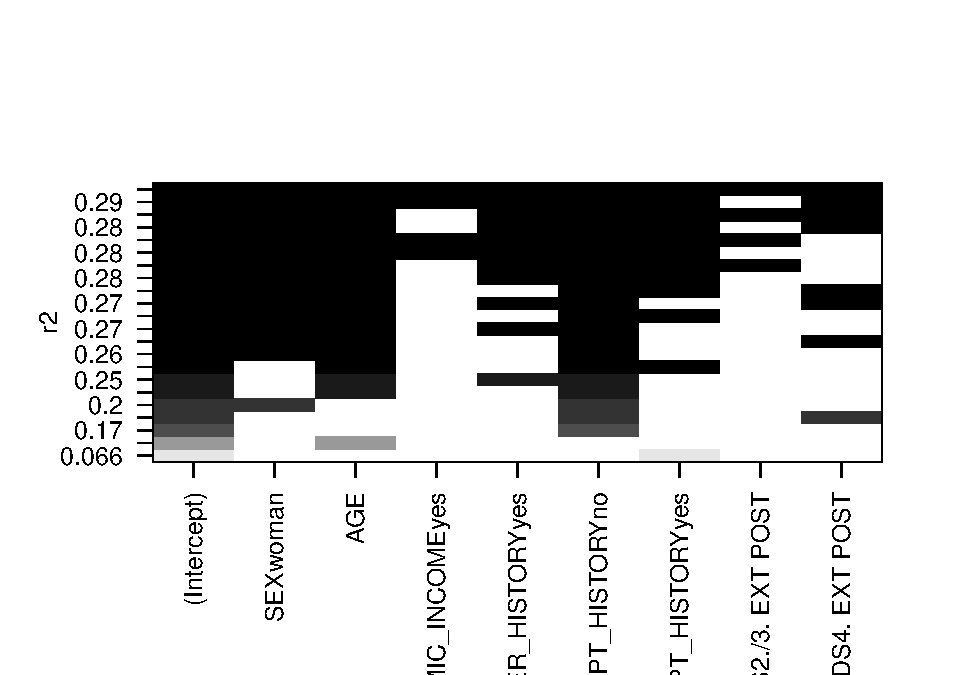
\includegraphics{Nexttry_files/figure-latex/unnamed-chunk-2-22.pdf}

\begin{Shaded}
\begin{Highlighting}[]
\FunctionTok{plot}\NormalTok{(leapsbestwith,}\AttributeTok{scale=}\StringTok{"adjr2"}\NormalTok{)}
\end{Highlighting}
\end{Shaded}

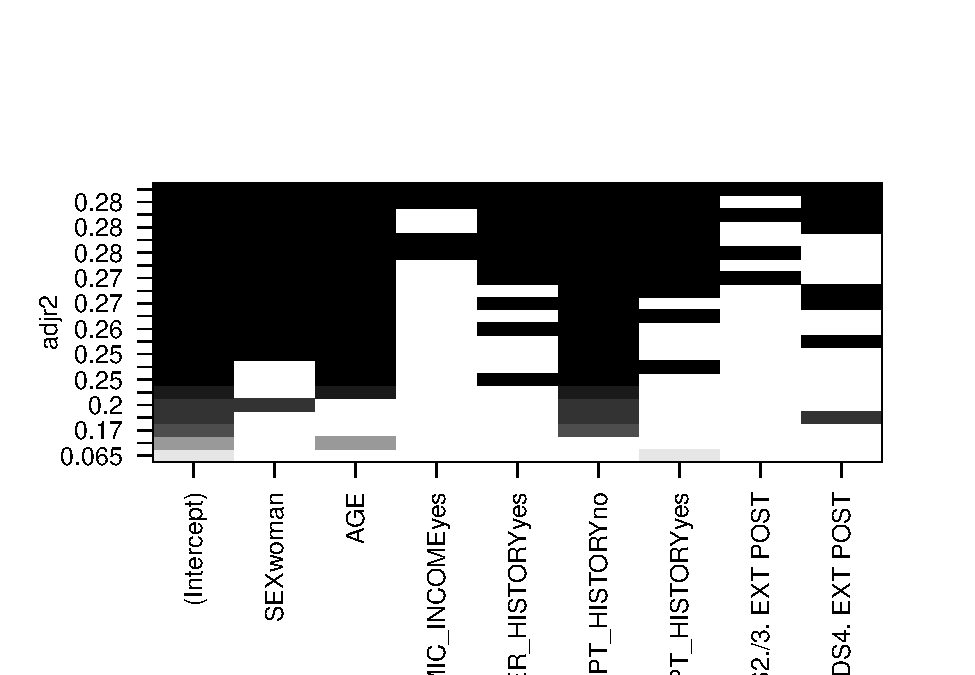
\includegraphics{Nexttry_files/figure-latex/unnamed-chunk-2-23.pdf}

\begin{Shaded}
\begin{Highlighting}[]
\CommentTok{\# First: AGE + SUIC\_ATTEMPT\_HISTORY (no):}
\NormalTok{besttwowithfirst}\OtherTok{\textless{}{-}}\FunctionTok{lm}\NormalTok{(DEPRESSION}\SpecialCharTok{\textasciitilde{}}\NormalTok{AGE}\SpecialCharTok{+}\NormalTok{SUIC\_ATTEMPT\_HISTORY,}\AttributeTok{data=}\NormalTok{table)}
\NormalTok{besttwowithfirst}
\end{Highlighting}
\end{Shaded}

\begin{verbatim}
## 
## Call:
## lm(formula = DEPRESSION ~ AGE + SUIC_ATTEMPT_HISTORY, data = table)
## 
## Coefficients:
##             (Intercept)                      AGE   SUIC_ATTEMPT_HISTORYno  
##                 28.0141                  -0.2424                  -7.5211  
## SUIC_ATTEMPT_HISTORYyes  
##                  5.6978
\end{verbatim}

\begin{Shaded}
\begin{Highlighting}[]
\FunctionTok{summary}\NormalTok{(besttwowithfirst)}
\end{Highlighting}
\end{Shaded}

\begin{verbatim}
## 
## Call:
## lm(formula = DEPRESSION ~ AGE + SUIC_ATTEMPT_HISTORY, data = table)
## 
## Residuals:
##     Min      1Q  Median      3Q     Max 
## -26.924  -6.675  -1.190   4.856  33.901 
## 
## Coefficients:
##                         Estimate Std. Error t value Pr(>|t|)    
## (Intercept)              28.0141     0.8981  31.191  < 2e-16 ***
## AGE                      -0.2424     0.0252  -9.621  < 2e-16 ***
## SUIC_ATTEMPT_HISTORYno   -7.5211     0.6838 -10.999  < 2e-16 ***
## SUIC_ATTEMPT_HISTORYyes   5.6978     1.2706   4.484 8.08e-06 ***
## ---
## Signif. codes:  0 '***' 0.001 '**' 0.01 '*' 0.05 '.' 0.1 ' ' 1
## 
## Residual standard error: 9.63 on 1096 degrees of freedom
## Multiple R-squared:  0.2495, Adjusted R-squared:  0.2474 
## F-statistic: 121.4 on 3 and 1096 DF,  p-value: < 2.2e-16
\end{verbatim}

\begin{Shaded}
\begin{Highlighting}[]
\FunctionTok{confint}\NormalTok{(besttwowithfirst)}
\end{Highlighting}
\end{Shaded}

\begin{verbatim}
##                              2.5 %     97.5 %
## (Intercept)             26.2518465 29.7763661
## AGE                     -0.2918707 -0.1929901
## SUIC_ATTEMPT_HISTORYno  -8.8628433 -6.1793996
## SUIC_ATTEMPT_HISTORYyes  3.2047351  8.1908180
\end{verbatim}

\begin{Shaded}
\begin{Highlighting}[]
\CommentTok{\# Second: SEX (woman) + SUIC\_ATTEMPT\_HISTORY (no):}
\NormalTok{besttwowithsecond}\OtherTok{\textless{}{-}}\FunctionTok{lm}\NormalTok{(DEPRESSION}\SpecialCharTok{\textasciitilde{}}\NormalTok{SEX}\SpecialCharTok{+}\NormalTok{SUIC\_ATTEMPT\_HISTORY,}\AttributeTok{data=}\NormalTok{table)}
\NormalTok{besttwowithsecond}
\end{Highlighting}
\end{Shaded}

\begin{verbatim}
## 
## Call:
## lm(formula = DEPRESSION ~ SEX + SUIC_ATTEMPT_HISTORY, data = table)
## 
## Coefficients:
##             (Intercept)                 SEXwoman   SUIC_ATTEMPT_HISTORYno  
##                  17.724                    4.235                   -8.531  
## SUIC_ATTEMPT_HISTORYyes  
##                   4.880
\end{verbatim}

\begin{Shaded}
\begin{Highlighting}[]
\FunctionTok{summary}\NormalTok{(besttwowithsecond)}
\end{Highlighting}
\end{Shaded}

\begin{verbatim}
## 
## Call:
## lm(formula = DEPRESSION ~ SEX + SUIC_ATTEMPT_HISTORY, data = table)
## 
## Residuals:
##     Min      1Q  Median      3Q     Max 
## -26.839  -6.959  -1.192   5.573  36.808 
## 
## Coefficients:
##                         Estimate Std. Error t value Pr(>|t|)    
## (Intercept)              17.7235     0.8669  20.444  < 2e-16 ***
## SEXwoman                  4.2351     0.7540   5.617 2.46e-08 ***
## SUIC_ATTEMPT_HISTORYno   -8.5315     0.6899 -12.367  < 2e-16 ***
## SUIC_ATTEMPT_HISTORYyes   4.8805     1.3042   3.742 0.000192 ***
## ---
## Signif. codes:  0 '***' 0.001 '**' 0.01 '*' 0.05 '.' 0.1 ' ' 1
## 
## Residual standard error: 9.888 on 1096 degrees of freedom
## Multiple R-squared:  0.2088, Adjusted R-squared:  0.2067 
## F-statistic: 96.44 on 3 and 1096 DF,  p-value: < 2.2e-16
\end{verbatim}

\begin{Shaded}
\begin{Highlighting}[]
\FunctionTok{confint}\NormalTok{(besttwowithsecond)}
\end{Highlighting}
\end{Shaded}

\begin{verbatim}
##                             2.5 %    97.5 %
## (Intercept)             16.022499 19.424514
## SEXwoman                 2.755633  5.714478
## SUIC_ATTEMPT_HISTORYno  -9.885088 -7.177814
## SUIC_ATTEMPT_HISTORYyes  2.321426  7.439514
\end{verbatim}

\begin{Shaded}
\begin{Highlighting}[]
\CommentTok{\# Third: SUIC\_ATTEMPT\_HISTORY (no) + SUB PERIODS (4. EXT POST):}
\NormalTok{besttwowiththird}\OtherTok{\textless{}{-}}\FunctionTok{lm}\NormalTok{(DEPRESSION}\SpecialCharTok{\textasciitilde{}}\NormalTok{SUIC\_ATTEMPT\_HISTORY}\SpecialCharTok{+}\NormalTok{SUB\_PERIODS,}\AttributeTok{data=}\NormalTok{table)}
\NormalTok{besttwowiththird}
\end{Highlighting}
\end{Shaded}

\begin{verbatim}
## 
## Call:
## lm(formula = DEPRESSION ~ SUIC_ATTEMPT_HISTORY + SUB_PERIODS, 
##     data = table)
## 
## Coefficients:
##               (Intercept)     SUIC_ATTEMPT_HISTORYno  
##                    19.326                     -8.785  
##   SUIC_ATTEMPT_HISTORYyes  SUB_PERIODS2./3. EXT POST  
##                     5.270                      1.888  
##    SUB_PERIODS4. EXT POST  
##                     3.377
\end{verbatim}

\begin{Shaded}
\begin{Highlighting}[]
\FunctionTok{summary}\NormalTok{(besttwowiththird)}
\end{Highlighting}
\end{Shaded}

\begin{verbatim}
## 
## Call:
## lm(formula = DEPRESSION ~ SUIC_ATTEMPT_HISTORY + SUB_PERIODS, 
##     data = table)
## 
## Residuals:
##     Min      1Q  Median      3Q     Max 
## -26.484  -6.918  -1.429   5.459  33.459 
## 
## Coefficients:
##                           Estimate Std. Error t value Pr(>|t|)    
## (Intercept)                19.3263     0.7323  26.390  < 2e-16 ***
## SUIC_ATTEMPT_HISTORYno     -8.7850     0.6902 -12.728  < 2e-16 ***
## SUIC_ATTEMPT_HISTORYyes     5.2697     1.3096   4.024 6.12e-05 ***
## SUB_PERIODS2./3. EXT POST   1.8879     0.8283   2.279   0.0228 *  
## SUB_PERIODS4. EXT POST      3.3771     0.6853   4.928 9.60e-07 ***
## ---
## Signif. codes:  0 '***' 0.001 '**' 0.01 '*' 0.05 '.' 0.1 ' ' 1
## 
## Residual standard error: 9.924 on 1095 degrees of freedom
## Multiple R-squared:  0.2037, Adjusted R-squared:  0.2008 
## F-statistic: 70.04 on 4 and 1095 DF,  p-value: < 2.2e-16
\end{verbatim}

\begin{Shaded}
\begin{Highlighting}[]
\FunctionTok{confint}\NormalTok{(besttwowiththird)}
\end{Highlighting}
\end{Shaded}

\begin{verbatim}
##                                 2.5 %    97.5 %
## (Intercept)                17.8893186 20.763222
## SUIC_ATTEMPT_HISTORYno    -10.1393637 -7.430695
## SUIC_ATTEMPT_HISTORYyes     2.7000714  7.839250
## SUB_PERIODS2./3. EXT POST   0.2627045  3.513014
## SUB_PERIODS4. EXT POST      2.0324452  4.721846
\end{verbatim}

\begin{Shaded}
\begin{Highlighting}[]
\DocumentationTok{\#\#\#\# ANXIETY{-}STATE:}
\CommentTok{\# Stepwise Regression}
\NormalTok{fitwith}\OtherTok{\textless{}{-}}\FunctionTok{lm}\NormalTok{(ANXIETY\_STATE}\SpecialCharTok{\textasciitilde{}}\NormalTok{SEX}\SpecialCharTok{+}\NormalTok{AGE}\SpecialCharTok{+}\NormalTok{PROVINCE}\SpecialCharTok{+}\NormalTok{EDUCATION}\SpecialCharTok{+}\NormalTok{ECONOMIC\_INCOME}\SpecialCharTok{+}\NormalTok{LIVING\_WITH\_SOMEBODY}\SpecialCharTok{+}\NormalTok{MENTAL\_DISORDER\_HISTORY}\SpecialCharTok{+}\NormalTok{SUIC\_ATTEMPT\_HISTORY}\SpecialCharTok{+}\NormalTok{SUB\_PERIODS,}\AttributeTok{data=}\NormalTok{table)}
\NormalTok{stepwith }\OtherTok{\textless{}{-}} \FunctionTok{stepAIC}\NormalTok{(fitwith, }\AttributeTok{trace=}\ConstantTok{TRUE}\NormalTok{,}\AttributeTok{direction=}\StringTok{"both"}\NormalTok{)}
\end{Highlighting}
\end{Shaded}

\begin{verbatim}
## Start:  AIC=5679.05
## ANXIETY_STATE ~ SEX + AGE + PROVINCE + EDUCATION + ECONOMIC_INCOME + 
##     LIVING_WITH_SOMEBODY + MENTAL_DISORDER_HISTORY + SUIC_ATTEMPT_HISTORY + 
##     SUB_PERIODS
## 
##                           Df Sum of Sq    RSS    AIC
## - PROVINCE                25    6695.3 184360 5669.7
## - EDUCATION                8    1678.0 179343 5673.4
## - ECONOMIC_INCOME          1       4.9 177670 5677.1
## - LIVING_WITH_SOMEBODY     1       6.9 177671 5677.1
## <none>                                 177665 5679.0
## - SUB_PERIODS              2     961.9 178627 5681.0
## - SEX                      1    2061.3 179726 5689.7
## - MENTAL_DISORDER_HISTORY  1    5918.7 183583 5713.1
## - AGE                      1    7049.9 184715 5719.9
## - SUIC_ATTEMPT_HISTORY     2   10052.6 187717 5735.6
## 
## Step:  AIC=5669.74
## ANXIETY_STATE ~ SEX + AGE + EDUCATION + ECONOMIC_INCOME + LIVING_WITH_SOMEBODY + 
##     MENTAL_DISORDER_HISTORY + SUIC_ATTEMPT_HISTORY + SUB_PERIODS
## 
##                           Df Sum of Sq    RSS    AIC
## - EDUCATION                8    1743.8 186104 5664.1
## - LIVING_WITH_SOMEBODY     1       2.0 184362 5667.7
## - ECONOMIC_INCOME          1      17.1 184377 5667.8
## <none>                                 184360 5669.7
## - SUB_PERIODS              2    1347.2 185707 5673.7
## + PROVINCE                25    6695.3 177665 5679.0
## - SEX                      1    2262.3 186622 5681.2
## - MENTAL_DISORDER_HISTORY  1    6257.0 190617 5704.5
## - AGE                      1    7220.3 191580 5710.0
## - SUIC_ATTEMPT_HISTORY     2   11618.0 195978 5733.0
## 
## Step:  AIC=5664.09
## ANXIETY_STATE ~ SEX + AGE + ECONOMIC_INCOME + LIVING_WITH_SOMEBODY + 
##     MENTAL_DISORDER_HISTORY + SUIC_ATTEMPT_HISTORY + SUB_PERIODS
## 
##                           Df Sum of Sq    RSS    AIC
## - ECONOMIC_INCOME          1       0.6 186104 5662.1
## - LIVING_WITH_SOMEBODY     1      25.7 186129 5662.2
## <none>                                 186104 5664.1
## - SUB_PERIODS              2    1218.8 187322 5667.3
## + EDUCATION                8    1743.8 184360 5669.7
## + PROVINCE                25    6761.0 179343 5673.4
## - SEX                      1    2172.9 188277 5674.9
## - MENTAL_DISORDER_HISTORY  1    6046.0 192150 5697.3
## - AGE                      1    7917.7 194021 5707.9
## - SUIC_ATTEMPT_HISTORY     2   11387.2 197491 5725.4
## 
## Step:  AIC=5662.1
## ANXIETY_STATE ~ SEX + AGE + LIVING_WITH_SOMEBODY + MENTAL_DISORDER_HISTORY + 
##     SUIC_ATTEMPT_HISTORY + SUB_PERIODS
## 
##                           Df Sum of Sq    RSS    AIC
## - LIVING_WITH_SOMEBODY     1      25.3 186130 5660.2
## <none>                                 186104 5662.1
## + ECONOMIC_INCOME          1       0.6 186104 5664.1
## - SUB_PERIODS              2    1218.3 187323 5665.3
## + EDUCATION                8    1727.3 184377 5667.8
## + PROVINCE                25    6761.1 179343 5671.4
## - SEX                      1    2172.4 188277 5672.9
## - MENTAL_DISORDER_HISTORY  1    6066.2 192171 5695.4
## - AGE                      1    8101.4 194206 5707.0
## - SUIC_ATTEMPT_HISTORY     2   11423.5 197528 5723.6
## 
## Step:  AIC=5660.25
## ANXIETY_STATE ~ SEX + AGE + MENTAL_DISORDER_HISTORY + SUIC_ATTEMPT_HISTORY + 
##     SUB_PERIODS
## 
##                           Df Sum of Sq    RSS    AIC
## <none>                                 186130 5660.2
## + LIVING_WITH_SOMEBODY     1      25.3 186104 5662.1
## + ECONOMIC_INCOME          1       0.2 186129 5662.2
## - SUB_PERIODS              2    1208.4 187338 5663.4
## + EDUCATION                8    1751.1 184378 5665.8
## + PROVINCE                25    6786.3 179343 5669.4
## - SEX                      1    2150.5 188280 5670.9
## - MENTAL_DISORDER_HISTORY  1    6143.0 192273 5694.0
## - AGE                      1    8144.7 194274 5705.4
## - SUIC_ATTEMPT_HISTORY     2   11470.5 197600 5722.0
\end{verbatim}

\begin{Shaded}
\begin{Highlighting}[]
\NormalTok{stepwith}
\end{Highlighting}
\end{Shaded}

\begin{verbatim}
## 
## Call:
## lm(formula = ANXIETY_STATE ~ SEX + AGE + MENTAL_DISORDER_HISTORY + 
##     SUIC_ATTEMPT_HISTORY + SUB_PERIODS, data = table)
## 
## Coefficients:
##                (Intercept)                    SEXwoman  
##                    37.5075                      3.5669  
##                        AGE  MENTAL_DISORDER_HISTORYyes  
##                    -0.2467                      5.5750  
##     SUIC_ATTEMPT_HISTORYno     SUIC_ATTEMPT_HISTORYyes  
##                    -6.0797                      4.5927  
##  SUB_PERIODS2./3. EXT POST      SUB_PERIODS4. EXT POST  
##                     2.6670                      1.9260
\end{verbatim}

\begin{Shaded}
\begin{Highlighting}[]
\NormalTok{stepwith}\SpecialCharTok{$}\NormalTok{anova }\CommentTok{\# display results}
\end{Highlighting}
\end{Shaded}

\begin{verbatim}
## Stepwise Model Path 
## Analysis of Deviance Table
## 
## Initial Model:
## ANXIETY_STATE ~ SEX + AGE + PROVINCE + EDUCATION + ECONOMIC_INCOME + 
##     LIVING_WITH_SOMEBODY + MENTAL_DISORDER_HISTORY + SUIC_ATTEMPT_HISTORY + 
##     SUB_PERIODS
## 
## Final Model:
## ANXIETY_STATE ~ SEX + AGE + MENTAL_DISORDER_HISTORY + SUIC_ATTEMPT_HISTORY + 
##     SUB_PERIODS
## 
## 
##                     Step Df     Deviance Resid. Df Resid. Dev      AIC
## 1                                             1057   177664.6 5679.046
## 2             - PROVINCE 25 6695.2611138      1082   184359.9 5669.737
## 3            - EDUCATION  8 1743.7974416      1090   186103.7 5664.093
## 4      - ECONOMIC_INCOME  1    0.6131264      1091   186104.3 5662.097
## 5 - LIVING_WITH_SOMEBODY  1   25.3363543      1092   186129.6 5660.246
\end{verbatim}

\begin{Shaded}
\begin{Highlighting}[]
\CommentTok{\# Stepwise Model Path }
\CommentTok{\# Analysis of Deviance Table}
\CommentTok{\# Initial Model: ANXIETY\_STATE \textasciitilde{} SEX + AGE + PROVINCE + EDUCATION + ECONOMIC\_INCOME + LIVING\_WITH\_SOMEBODY + MENTAL\_DISORDER\_HISTORY + SUIC\_ATTEMPT\_HISTORY + SUB\_PERIODS}
\CommentTok{\# Start:  AIC = 5679.05}
\CommentTok{\# Final Model: ANXIETY\_STATE \textasciitilde{} SEX + AGE + MENTAL\_DISORDER\_HISTORY + SUIC\_ATTEMPT\_HISTORY + SUB\_PERIODS}
\CommentTok{\# Stepwith:  AIC = 5660.25}
\FunctionTok{summary}\NormalTok{(stepwith)}
\end{Highlighting}
\end{Shaded}

\begin{verbatim}
## 
## Call:
## lm(formula = ANXIETY_STATE ~ SEX + AGE + MENTAL_DISORDER_HISTORY + 
##     SUIC_ATTEMPT_HISTORY + SUB_PERIODS, data = table)
## 
## Residuals:
##     Min      1Q  Median      3Q     Max 
## -42.888  -9.256  -0.957   9.615  39.500 
## 
## Coefficients:
##                            Estimate Std. Error t value Pr(>|t|)    
## (Intercept)                37.50746    1.75346  21.391  < 2e-16 ***
## SEXwoman                    3.56692    1.00420   3.552 0.000399 ***
## AGE                        -0.24668    0.03569  -6.913 8.08e-12 ***
## MENTAL_DISORDER_HISTORYyes  5.57505    0.92866   6.003 2.63e-09 ***
## SUIC_ATTEMPT_HISTORYno     -6.07967    0.95292  -6.380 2.61e-10 ***
## SUIC_ATTEMPT_HISTORYyes     4.59266    1.73290   2.650 0.008159 ** 
## SUB_PERIODS2./3. EXT POST   2.66701    1.09080   2.445 0.014642 *  
## SUB_PERIODS4. EXT POST      1.92599    0.92985   2.071 0.038566 *  
## ---
## Signif. codes:  0 '***' 0.001 '**' 0.01 '*' 0.05 '.' 0.1 ' ' 1
## 
## Residual standard error: 13.06 on 1092 degrees of freedom
## Multiple R-squared:  0.1915, Adjusted R-squared:  0.1863 
## F-statistic: 36.95 on 7 and 1092 DF,  p-value: < 2.2e-16
\end{verbatim}

\begin{Shaded}
\begin{Highlighting}[]
\CommentTok{\# 95\% Confidence interval of best{-}fitted model:}
\FunctionTok{confint}\NormalTok{(stepwith)}
\end{Highlighting}
\end{Shaded}

\begin{verbatim}
##                                 2.5 %     97.5 %
## (Intercept)                34.0669382 40.9479900
## SEXwoman                    1.5965481  5.5373004
## AGE                        -0.3167030 -0.1766614
## MENTAL_DISORDER_HISTORYyes  3.7528959  7.3972016
## SUIC_ATTEMPT_HISTORYno     -7.9494314 -4.2099141
## SUIC_ATTEMPT_HISTORYyes     1.1924686  7.9928562
## SUB_PERIODS2./3. EXT POST   0.5267105  4.8073133
## SUB_PERIODS4. EXT POST      0.1014973  3.7504751
\end{verbatim}

\begin{Shaded}
\begin{Highlighting}[]
\CommentTok{\# ERROR RATE of best{-}fitted model:}
\FunctionTok{sigma}\NormalTok{(stepwith)}\SpecialCharTok{/}\FunctionTok{mean}\NormalTok{(table}\SpecialCharTok{$}\NormalTok{ANXIETY\_STATE)}
\end{Highlighting}
\end{Shaded}

\begin{verbatim}
## [1] 0.4108702
\end{verbatim}

\begin{Shaded}
\begin{Highlighting}[]
\CommentTok{\# 0.4108702}
\CommentTok{\# In our multiple regression example, the Residual Standard Error (RSE) or sigma is 13.06 corresponding to 41\% error rate.}

\FunctionTok{par}\NormalTok{(}\AttributeTok{mfrow=}\FunctionTok{c}\NormalTok{(}\DecValTok{2}\NormalTok{,}\DecValTok{2}\NormalTok{))}
\CommentTok{\# Figure S6 (Supplementary material)}
\FunctionTok{plot}\NormalTok{(stepwith)}
\end{Highlighting}
\end{Shaded}

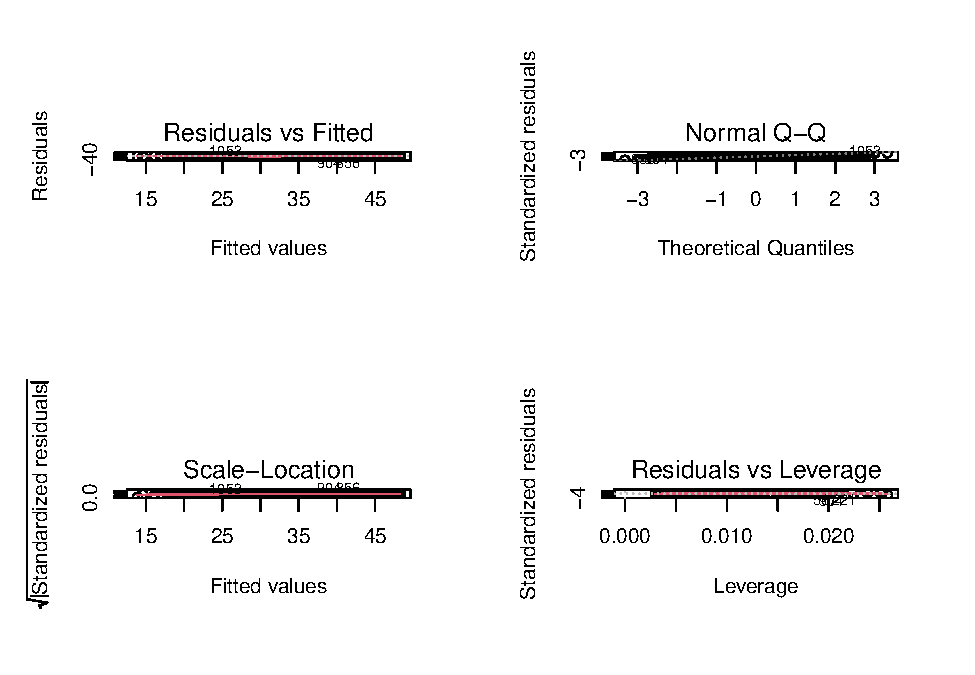
\includegraphics{Nexttry_files/figure-latex/unnamed-chunk-2-24.pdf}

\begin{Shaded}
\begin{Highlighting}[]
\FunctionTok{par}\NormalTok{(}\AttributeTok{mfrow=}\FunctionTok{c}\NormalTok{(}\DecValTok{1}\NormalTok{,}\DecValTok{1}\NormalTok{))}


\CommentTok{\# TABLE 1:}

\CommentTok{\# Model 1: INITIAL MODEL:}
\NormalTok{model1}\OtherTok{\textless{}{-}}\FunctionTok{lm}\NormalTok{(ANXIETY\_STATE}\SpecialCharTok{\textasciitilde{}}\NormalTok{SEX}\SpecialCharTok{+}\NormalTok{AGE}\SpecialCharTok{+}\NormalTok{PROVINCE}\SpecialCharTok{+}\NormalTok{EDUCATION}\SpecialCharTok{+}\NormalTok{ECONOMIC\_INCOME}\SpecialCharTok{+}\NormalTok{LIVING\_WITH\_SOMEBODY}\SpecialCharTok{+}\NormalTok{MENTAL\_DISORDER\_HISTORY}\SpecialCharTok{+}\NormalTok{SUIC\_ATTEMPT\_HISTORY}\SpecialCharTok{+}\NormalTok{SUB\_PERIODS,}\AttributeTok{data=}\NormalTok{table)}
\FunctionTok{summary}\NormalTok{(model1)}
\end{Highlighting}
\end{Shaded}

\begin{verbatim}
## 
## Call:
## lm(formula = ANXIETY_STATE ~ SEX + AGE + PROVINCE + EDUCATION + 
##     ECONOMIC_INCOME + LIVING_WITH_SOMEBODY + MENTAL_DISORDER_HISTORY + 
##     SUIC_ATTEMPT_HISTORY + SUB_PERIODS, data = table)
## 
## Residuals:
##     Min      1Q  Median      3Q     Max 
## -41.477  -9.057  -0.506   9.018  39.250 
## 
## Coefficients:
##                                             Estimate Std. Error t value
## (Intercept)                                 19.89283    9.56535   2.080
## SEXwoman                                     3.57949    1.02215   3.502
## AGE                                         -0.25965    0.04009  -6.476
## PROVINCECABA (Buenos Aires capital)          0.33719    1.59179   0.212
## PROVINCECatamarca                            5.10875    9.38377   0.544
## PROVINCEChaco                               -1.92192    5.02327  -0.383
## PROVINCEChubut                              -2.35077    6.57489  -0.358
## PROVINCECórdoba                             -3.45015    1.23164  -2.801
## PROVINCECorrientes                         -12.63421    5.89774  -2.142
## PROVINCEEntre Ríos                          -3.61585    3.51548  -1.029
## PROVINCEFormosa                              6.21207    7.57915   0.820
## PROVINCEJujuy                               -2.56294    2.42337  -1.058
## PROVINCELa Pampa                           -13.02703    4.70542  -2.769
## PROVINCELa Rioja                           -23.84734   13.08921  -1.822
## PROVINCEMendoza                              2.52823    3.31661   0.762
## PROVINCEMisiones                            -6.85122    3.60500  -1.900
## PROVINCENeuquén                             -7.07254    4.56333  -1.550
## PROVINCEother                               -2.98791    3.24800  -0.920
## PROVINCEOtro                                 3.07520    7.65533   0.402
## PROVINCERío Negro                            3.34309    6.57694   0.508
## PROVINCESalta                                2.61668    3.88231   0.674
## PROVINCESan Juan                            -7.81884    6.61909  -1.181
## PROVINCESan Luis                            21.47288   13.07624   1.642
## PROVINCESanta Cruz                           2.47300    9.24914   0.267
## PROVINCESanta Fe                            -3.21944    1.22485  -2.628
## PROVINCESantiago del Estero                 -1.58396    3.60668  -0.439
## PROVINCETierra del Fuego                    -2.29507    3.14980  -0.729
## PROVINCETucumán                             -2.02395    2.75068  -0.736
## EDUCATIONCompleted high school              19.28739    9.34707   2.063
## EDUCATIONCompleted postgraduate             20.16787    9.34601   2.158
## EDUCATIONCompleted tertiary or university   19.70575    9.30144   2.119
## EDUCATIONIncomplete elementary school       26.84940   15.97422   1.681
## EDUCATIONIncomplete high school             22.14432    9.65382   2.294
## EDUCATIONIncomplete postgraduate            22.79042    9.38319   2.429
## EDUCATIONIncomplete tertiary or university  19.57363    9.29082   2.107
## EDUCATIONOtro                               19.71503   13.25588   1.487
## ECONOMIC_INCOMEyes                          -0.18975    1.11134  -0.171
## LIVING_WITH_SOMEBODYyes                      0.23270    1.15084   0.202
## MENTAL_DISORDER_HISTORYyes                   5.56871    0.93844   5.934
## SUIC_ATTEMPT_HISTORYno                      -5.84712    0.96916  -6.033
## SUIC_ATTEMPT_HISTORYyes                      4.42879    1.74337   2.540
## SUB_PERIODS2./3. EXT POST                    2.29225    1.15756   1.980
## SUB_PERIODS4. EXT POST                       2.25811    1.06930   2.112
##                                            Pr(>|t|)    
## (Intercept)                                0.037796 *  
## SEXwoman                                   0.000481 ***
## AGE                                        1.44e-10 ***
## PROVINCECABA (Buenos Aires capital)        0.832281    
## PROVINCECatamarca                          0.586264    
## PROVINCEChaco                              0.702091    
## PROVINCEChubut                             0.720761    
## PROVINCECórdoba                            0.005183 ** 
## PROVINCECorrientes                         0.032405 *  
## PROVINCEEntre Ríos                         0.303926    
## PROVINCEFormosa                            0.412614    
## PROVINCEJujuy                              0.290482    
## PROVINCELa Pampa                           0.005730 ** 
## PROVINCELa Rioja                           0.068751 .  
## PROVINCEMendoza                            0.446055    
## PROVINCEMisiones                           0.057643 .  
## PROVINCENeuquén                            0.121473    
## PROVINCEother                              0.357824    
## PROVINCEOtro                               0.687980    
## PROVINCERío Negro                          0.611346    
## PROVINCESalta                              0.500459    
## PROVINCESan Juan                           0.237767    
## PROVINCESan Luis                           0.100861    
## PROVINCESanta Cruz                         0.789231    
## PROVINCESanta Fe                           0.008702 ** 
## PROVINCESantiago del Estero                0.660626    
## PROVINCETierra del Fuego                   0.466384    
## PROVINCETucumán                            0.462016    
## EDUCATIONCompleted high school             0.039312 *  
## EDUCATIONCompleted postgraduate            0.031159 *  
## EDUCATIONCompleted tertiary or university  0.034360 *  
## EDUCATIONIncomplete elementary school      0.093098 .  
## EDUCATIONIncomplete high school            0.021995 *  
## EDUCATIONIncomplete postgraduate           0.015312 *  
## EDUCATIONIncomplete tertiary or university 0.035373 *  
## EDUCATIONOtro                              0.137243    
## ECONOMIC_INCOMEyes                         0.864463    
## LIVING_WITH_SOMEBODYyes                    0.839801    
## MENTAL_DISORDER_HISTORYyes                 4.00e-09 ***
## SUIC_ATTEMPT_HISTORYno                     2.22e-09 ***
## SUIC_ATTEMPT_HISTORYyes                    0.011216 *  
## SUB_PERIODS2./3. EXT POST                  0.047935 *  
## SUB_PERIODS4. EXT POST                     0.034940 *  
## ---
## Signif. codes:  0 '***' 0.001 '**' 0.01 '*' 0.05 '.' 0.1 ' ' 1
## 
## Residual standard error: 12.96 on 1057 degrees of freedom
## Multiple R-squared:  0.2283, Adjusted R-squared:  0.1976 
## F-statistic: 7.445 on 42 and 1057 DF,  p-value: < 2.2e-16
\end{verbatim}

\begin{Shaded}
\begin{Highlighting}[]
\CommentTok{\# YES significative p{-}value \textless{} 2.2e{-}16}

\CommentTok{\# Model 2 eliminates PROVINCE:}
\NormalTok{model2}\OtherTok{\textless{}{-}}\FunctionTok{lm}\NormalTok{(ANXIETY\_STATE}\SpecialCharTok{\textasciitilde{}}\NormalTok{SEX}\SpecialCharTok{+}\NormalTok{AGE}\SpecialCharTok{+}\NormalTok{EDUCATION}\SpecialCharTok{+}\NormalTok{ECONOMIC\_INCOME}\SpecialCharTok{+}\NormalTok{LIVING\_WITH\_SOMEBODY}\SpecialCharTok{+}\NormalTok{MENTAL\_DISORDER\_HISTORY}\SpecialCharTok{+}\NormalTok{SUIC\_ATTEMPT\_HISTORY}\SpecialCharTok{+}\NormalTok{SUB\_PERIODS,}\AttributeTok{data=}\NormalTok{table)}
\FunctionTok{summary}\NormalTok{(model2)}
\end{Highlighting}
\end{Shaded}

\begin{verbatim}
## 
## Call:
## lm(formula = ANXIETY_STATE ~ SEX + AGE + EDUCATION + ECONOMIC_INCOME + 
##     LIVING_WITH_SOMEBODY + MENTAL_DISORDER_HISTORY + SUIC_ATTEMPT_HISTORY + 
##     SUB_PERIODS, data = table)
## 
## Residuals:
##     Min      1Q  Median      3Q     Max 
## -42.598  -9.059  -0.913   9.486  38.541 
## 
## Coefficients:
##                                            Estimate Std. Error t value Pr(>|t|)
## (Intercept)                                18.23288    9.59898   1.899 0.057770
## SEXwoman                                    3.68573    1.01149   3.644 0.000281
## AGE                                        -0.25601    0.03933  -6.510 1.15e-10
## EDUCATIONCompleted high school             19.19709    9.39399   2.044 0.041240
## EDUCATIONCompleted postgraduate            20.04070    9.37726   2.137 0.032809
## EDUCATIONCompleted tertiary or university  19.84627    9.34777   2.123 0.033972
## EDUCATIONIncomplete elementary school      25.91353   16.06586   1.613 0.107046
## EDUCATIONIncomplete high school            21.82096    9.68481   2.253 0.024452
## EDUCATIONIncomplete postgraduate           22.87390    9.42458   2.427 0.015385
## EDUCATIONIncomplete tertiary or university 19.47661    9.33833   2.086 0.037243
## EDUCATIONOtro                              16.67835   13.10442   1.273 0.203388
## ECONOMIC_INCOMEyes                         -0.35179    1.10994  -0.317 0.751346
## LIVING_WITH_SOMEBODYyes                    -0.12254    1.14059  -0.107 0.914461
## MENTAL_DISORDER_HISTORYyes                  5.66844    0.93541   6.060 1.88e-09
## SUIC_ATTEMPT_HISTORYno                     -6.29768    0.96299  -6.540 9.49e-11
## SUIC_ATTEMPT_HISTORYyes                     4.40224    1.74179   2.527 0.011632
## SUB_PERIODS2./3. EXT POST                   2.74132    1.09398   2.506 0.012363
## SUB_PERIODS4. EXT POST                      2.15251    0.93841   2.294 0.021994
##                                               
## (Intercept)                                .  
## SEXwoman                                   ***
## AGE                                        ***
## EDUCATIONCompleted high school             *  
## EDUCATIONCompleted postgraduate            *  
## EDUCATIONCompleted tertiary or university  *  
## EDUCATIONIncomplete elementary school         
## EDUCATIONIncomplete high school            *  
## EDUCATIONIncomplete postgraduate           *  
## EDUCATIONIncomplete tertiary or university *  
## EDUCATIONOtro                                 
## ECONOMIC_INCOMEyes                            
## LIVING_WITH_SOMEBODYyes                       
## MENTAL_DISORDER_HISTORYyes                 ***
## SUIC_ATTEMPT_HISTORYno                     ***
## SUIC_ATTEMPT_HISTORYyes                    *  
## SUB_PERIODS2./3. EXT POST                  *  
## SUB_PERIODS4. EXT POST                     *  
## ---
## Signif. codes:  0 '***' 0.001 '**' 0.01 '*' 0.05 '.' 0.1 ' ' 1
## 
## Residual standard error: 13.05 on 1082 degrees of freedom
## Multiple R-squared:  0.1992, Adjusted R-squared:  0.1866 
## F-statistic: 15.83 on 17 and 1082 DF,  p-value: < 2.2e-16
\end{verbatim}

\begin{Shaded}
\begin{Highlighting}[]
\CommentTok{\# YES significative p{-}value \textless{} 2.2e{-}16}

\CommentTok{\# Model 3 eliminates EDUCATION:}
\NormalTok{model3}\OtherTok{\textless{}{-}}\FunctionTok{lm}\NormalTok{(ANXIETY\_STATE}\SpecialCharTok{\textasciitilde{}}\NormalTok{SEX}\SpecialCharTok{+}\NormalTok{AGE}\SpecialCharTok{+}\NormalTok{ECONOMIC\_INCOME}\SpecialCharTok{+}\NormalTok{LIVING\_WITH\_SOMEBODY}\SpecialCharTok{+}\NormalTok{MENTAL\_DISORDER\_HISTORY}\SpecialCharTok{+}\NormalTok{SUIC\_ATTEMPT\_HISTORY}\SpecialCharTok{+}\NormalTok{SUB\_PERIODS,}\AttributeTok{data=}\NormalTok{table)}
\FunctionTok{summary}\NormalTok{(model3)}
\end{Highlighting}
\end{Shaded}

\begin{verbatim}
## 
## Call:
## lm(formula = ANXIETY_STATE ~ SEX + AGE + ECONOMIC_INCOME + LIVING_WITH_SOMEBODY + 
##     MENTAL_DISORDER_HISTORY + SUIC_ATTEMPT_HISTORY + SUB_PERIODS, 
##     data = table)
## 
## Residuals:
##     Min      1Q  Median      3Q     Max 
## -42.818  -9.321  -0.951   9.687  39.612 
## 
## Coefficients:
##                            Estimate Std. Error t value Pr(>|t|)    
## (Intercept)                37.97130    2.20761  17.200  < 2e-16 ***
## SEXwoman                    3.59413    1.00747   3.567 0.000376 ***
## AGE                        -0.24842    0.03648  -6.810 1.61e-11 ***
## ECONOMIC_INCOMEyes         -0.06529    1.08955  -0.060 0.952226    
## LIVING_WITH_SOMEBODYyes    -0.43989    1.13316  -0.388 0.697943    
## MENTAL_DISORDER_HISTORYyes  5.54907    0.93250   5.951 3.59e-09 ***
## SUIC_ATTEMPT_HISTORYno     -6.07643    0.95400  -6.369 2.79e-10 ***
## SUIC_ATTEMPT_HISTORYyes     4.56136    1.73714   2.626 0.008766 ** 
## SUB_PERIODS2./3. EXT POST   2.68491    1.09269   2.457 0.014159 *  
## SUB_PERIODS4. EXT POST      1.92875    0.93084   2.072 0.038496 *  
## ---
## Signif. codes:  0 '***' 0.001 '**' 0.01 '*' 0.05 '.' 0.1 ' ' 1
## 
## Residual standard error: 13.07 on 1090 degrees of freedom
## Multiple R-squared:  0.1916, Adjusted R-squared:  0.185 
## F-statistic: 28.71 on 9 and 1090 DF,  p-value: < 2.2e-16
\end{verbatim}

\begin{Shaded}
\begin{Highlighting}[]
\CommentTok{\# YES significative p{-}value \textless{} 2.2e{-}16}

\CommentTok{\# Model 4 eliminates ECONOMIC\_INCOME:}
\NormalTok{model4}\OtherTok{\textless{}{-}}\FunctionTok{lm}\NormalTok{(ANXIETY\_STATE}\SpecialCharTok{\textasciitilde{}}\NormalTok{SEX}\SpecialCharTok{+}\NormalTok{AGE}\SpecialCharTok{+}\NormalTok{LIVING\_WITH\_SOMEBODY}\SpecialCharTok{+}\NormalTok{MENTAL\_DISORDER\_HISTORY}\SpecialCharTok{+}\NormalTok{SUIC\_ATTEMPT\_HISTORY}\SpecialCharTok{+}\NormalTok{SUB\_PERIODS,}\AttributeTok{data=}\NormalTok{table)}
\FunctionTok{summary}\NormalTok{(model4)}
\end{Highlighting}
\end{Shaded}

\begin{verbatim}
## 
## Call:
## lm(formula = ANXIETY_STATE ~ SEX + AGE + LIVING_WITH_SOMEBODY + 
##     MENTAL_DISORDER_HISTORY + SUIC_ATTEMPT_HISTORY + SUB_PERIODS, 
##     data = table)
## 
## Residuals:
##     Min      1Q  Median      3Q     Max 
## -42.835  -9.324  -0.961   9.690  39.606 
## 
## Coefficients:
##                            Estimate Std. Error t value Pr(>|t|)    
## (Intercept)                37.92393    2.06028  18.407  < 2e-16 ***
## SEXwoman                    3.59330    1.00692   3.569 0.000374 ***
## AGE                        -0.24873    0.03609  -6.892 9.32e-12 ***
## LIVING_WITH_SOMEBODYyes    -0.43567    1.13044  -0.385 0.700020    
## MENTAL_DISORDER_HISTORYyes  5.55179    0.93098   5.963 3.33e-09 ***
## SUIC_ATTEMPT_HISTORYno     -6.07776    0.95330  -6.375 2.69e-10 ***
## SUIC_ATTEMPT_HISTORYyes     4.56544    1.73502   2.631 0.008625 ** 
## SUB_PERIODS2./3. EXT POST   2.68450    1.09217   2.458 0.014128 *  
## SUB_PERIODS4. EXT POST      1.92760    0.93022   2.072 0.038481 *  
## ---
## Signif. codes:  0 '***' 0.001 '**' 0.01 '*' 0.05 '.' 0.1 ' ' 1
## 
## Residual standard error: 13.06 on 1091 degrees of freedom
## Multiple R-squared:  0.1916, Adjusted R-squared:  0.1857 
## F-statistic: 32.33 on 8 and 1091 DF,  p-value: < 2.2e-16
\end{verbatim}

\begin{Shaded}
\begin{Highlighting}[]
\CommentTok{\# YES significative p{-}value \textless{} 2.2e{-}16}

\CommentTok{\# Model 5 eliminates LIVING\_WITH\_SOMEBODY:}
\NormalTok{model5}\OtherTok{\textless{}{-}}\FunctionTok{lm}\NormalTok{(ANXIETY\_STATE}\SpecialCharTok{\textasciitilde{}}\NormalTok{SEX}\SpecialCharTok{+}\NormalTok{AGE}\SpecialCharTok{+}\NormalTok{MENTAL\_DISORDER\_HISTORY}\SpecialCharTok{+}\NormalTok{SUIC\_ATTEMPT\_HISTORY}\SpecialCharTok{+}\NormalTok{SUB\_PERIODS,}\AttributeTok{data=}\NormalTok{table)}
\FunctionTok{summary}\NormalTok{(model5)}
\end{Highlighting}
\end{Shaded}

\begin{verbatim}
## 
## Call:
## lm(formula = ANXIETY_STATE ~ SEX + AGE + MENTAL_DISORDER_HISTORY + 
##     SUIC_ATTEMPT_HISTORY + SUB_PERIODS, data = table)
## 
## Residuals:
##     Min      1Q  Median      3Q     Max 
## -42.888  -9.256  -0.957   9.615  39.500 
## 
## Coefficients:
##                            Estimate Std. Error t value Pr(>|t|)    
## (Intercept)                37.50746    1.75346  21.391  < 2e-16 ***
## SEXwoman                    3.56692    1.00420   3.552 0.000399 ***
## AGE                        -0.24668    0.03569  -6.913 8.08e-12 ***
## MENTAL_DISORDER_HISTORYyes  5.57505    0.92866   6.003 2.63e-09 ***
## SUIC_ATTEMPT_HISTORYno     -6.07967    0.95292  -6.380 2.61e-10 ***
## SUIC_ATTEMPT_HISTORYyes     4.59266    1.73290   2.650 0.008159 ** 
## SUB_PERIODS2./3. EXT POST   2.66701    1.09080   2.445 0.014642 *  
## SUB_PERIODS4. EXT POST      1.92599    0.92985   2.071 0.038566 *  
## ---
## Signif. codes:  0 '***' 0.001 '**' 0.01 '*' 0.05 '.' 0.1 ' ' 1
## 
## Residual standard error: 13.06 on 1092 degrees of freedom
## Multiple R-squared:  0.1915, Adjusted R-squared:  0.1863 
## F-statistic: 36.95 on 7 and 1092 DF,  p-value: < 2.2e-16
\end{verbatim}

\begin{Shaded}
\begin{Highlighting}[]
\CommentTok{\# YES significative p{-}value \textless{} 2.2e{-}16}



\DocumentationTok{\#\#\#\#\#\#\#\#\#\#\#\#\#\#\#\#}
\DocumentationTok{\#\# Considering the predictors included in the best{-}fitted model (i.e., stepwith) in this group, we analyzed the smallest possible linear model for each specific MHS indicator by means of all two{-}predictor combinations.  }
\CommentTok{\# We performed all{-}subsets regression using the regsubsets() function from the leaps package.}
\CommentTok{\# We analyzed the three best models for two{-}predictor subset sizes.}

\NormalTok{leapsbestwith}\OtherTok{\textless{}{-}}\FunctionTok{regsubsets}\NormalTok{(ANXIETY\_STATE}\SpecialCharTok{\textasciitilde{}}\NormalTok{SEX}\SpecialCharTok{+}\NormalTok{AGE}\SpecialCharTok{+}\NormalTok{MENTAL\_DISORDER\_HISTORY}\SpecialCharTok{+}\NormalTok{SUIC\_ATTEMPT\_HISTORY}\SpecialCharTok{+}\NormalTok{SUB\_PERIODS,}\AttributeTok{data=}\NormalTok{table,}\AttributeTok{nbest=}\DecValTok{3}\NormalTok{)}
\FunctionTok{summary}\NormalTok{(leapsbestwith)}
\end{Highlighting}
\end{Shaded}

\begin{verbatim}
## Subset selection object
## Call: regsubsets.formula(ANXIETY_STATE ~ SEX + AGE + MENTAL_DISORDER_HISTORY + 
##     SUIC_ATTEMPT_HISTORY + SUB_PERIODS, data = table, nbest = 3)
## 7 Variables  (and intercept)
##                            Forced in Forced out
## SEXwoman                       FALSE      FALSE
## AGE                            FALSE      FALSE
## MENTAL_DISORDER_HISTORYyes     FALSE      FALSE
## SUIC_ATTEMPT_HISTORYno         FALSE      FALSE
## SUIC_ATTEMPT_HISTORYyes        FALSE      FALSE
## SUB_PERIODS2./3. EXT POST      FALSE      FALSE
## SUB_PERIODS4. EXT POST         FALSE      FALSE
## 3 subsets of each size up to 7
## Selection Algorithm: exhaustive
##          SEXwoman AGE MENTAL_DISORDER_HISTORYyes SUIC_ATTEMPT_HISTORYno
## 1  ( 1 ) " "      " " " "                        "*"                   
## 1  ( 2 ) " "      "*" " "                        " "                   
## 1  ( 3 ) " "      " " "*"                        " "                   
## 2  ( 1 ) " "      "*" " "                        "*"                   
## 2  ( 2 ) " "      " " "*"                        "*"                   
## 2  ( 3 ) " "      "*" "*"                        " "                   
## 3  ( 1 ) " "      "*" "*"                        "*"                   
## 3  ( 2 ) "*"      "*" " "                        "*"                   
## 3  ( 3 ) " "      "*" " "                        "*"                   
## 4  ( 1 ) "*"      "*" "*"                        "*"                   
## 4  ( 2 ) " "      "*" "*"                        "*"                   
## 4  ( 3 ) " "      "*" "*"                        "*"                   
## 5  ( 1 ) "*"      "*" "*"                        "*"                   
## 5  ( 2 ) "*"      "*" "*"                        "*"                   
## 5  ( 3 ) "*"      "*" "*"                        "*"                   
## 6  ( 1 ) "*"      "*" "*"                        "*"                   
## 6  ( 2 ) "*"      "*" "*"                        "*"                   
## 6  ( 3 ) "*"      "*" "*"                        "*"                   
## 7  ( 1 ) "*"      "*" "*"                        "*"                   
##          SUIC_ATTEMPT_HISTORYyes SUB_PERIODS2./3. EXT POST
## 1  ( 1 ) " "                     " "                      
## 1  ( 2 ) " "                     " "                      
## 1  ( 3 ) " "                     " "                      
## 2  ( 1 ) " "                     " "                      
## 2  ( 2 ) " "                     " "                      
## 2  ( 3 ) " "                     " "                      
## 3  ( 1 ) " "                     " "                      
## 3  ( 2 ) " "                     " "                      
## 3  ( 3 ) "*"                     " "                      
## 4  ( 1 ) " "                     " "                      
## 4  ( 2 ) "*"                     " "                      
## 4  ( 3 ) " "                     "*"                      
## 5  ( 1 ) "*"                     " "                      
## 5  ( 2 ) " "                     "*"                      
## 5  ( 3 ) " "                     " "                      
## 6  ( 1 ) "*"                     "*"                      
## 6  ( 2 ) "*"                     " "                      
## 6  ( 3 ) " "                     "*"                      
## 7  ( 1 ) "*"                     "*"                      
##          SUB_PERIODS4. EXT POST
## 1  ( 1 ) " "                   
## 1  ( 2 ) " "                   
## 1  ( 3 ) " "                   
## 2  ( 1 ) " "                   
## 2  ( 2 ) " "                   
## 2  ( 3 ) " "                   
## 3  ( 1 ) " "                   
## 3  ( 2 ) " "                   
## 3  ( 3 ) " "                   
## 4  ( 1 ) " "                   
## 4  ( 2 ) " "                   
## 4  ( 3 ) " "                   
## 5  ( 1 ) " "                   
## 5  ( 2 ) " "                   
## 5  ( 3 ) "*"                   
## 6  ( 1 ) " "                   
## 6  ( 2 ) "*"                   
## 6  ( 3 ) "*"                   
## 7  ( 1 ) "*"
\end{verbatim}

\begin{Shaded}
\begin{Highlighting}[]
\CommentTok{\# The best two{-}predictors model was: ANXIETY\_STATE \textasciitilde{} AGE + SUIC\_ATTEMPT\_HISTORY==no}

\FunctionTok{plot}\NormalTok{(leapsbestwith,}\AttributeTok{scale=}\StringTok{"r2"}\NormalTok{)}
\end{Highlighting}
\end{Shaded}

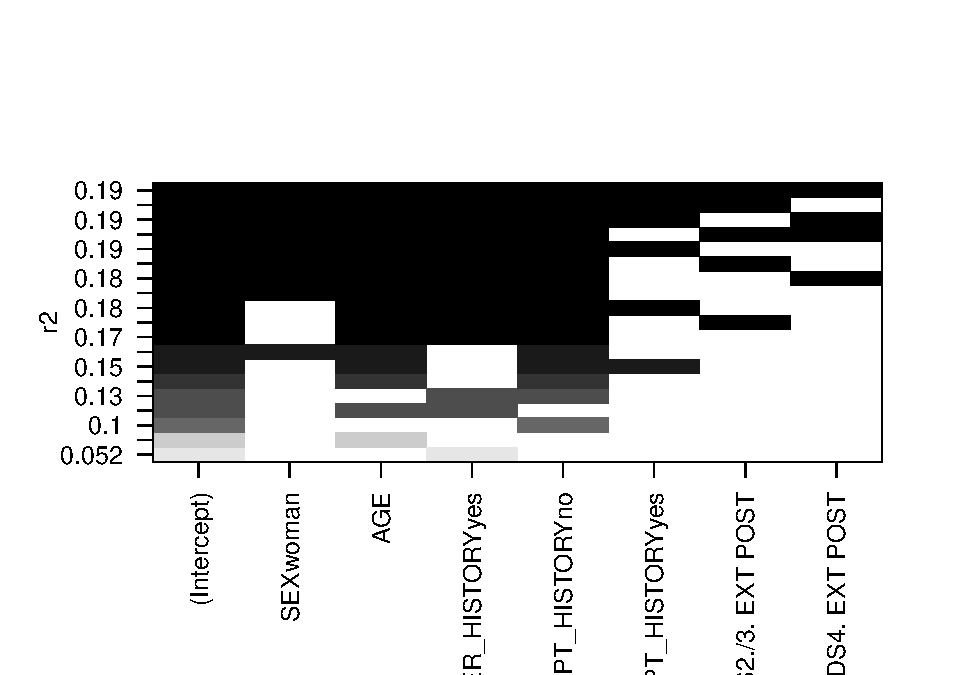
\includegraphics{Nexttry_files/figure-latex/unnamed-chunk-2-25.pdf}

\begin{Shaded}
\begin{Highlighting}[]
\FunctionTok{plot}\NormalTok{(leapsbestwith,}\AttributeTok{scale=}\StringTok{"adjr2"}\NormalTok{)}
\end{Highlighting}
\end{Shaded}

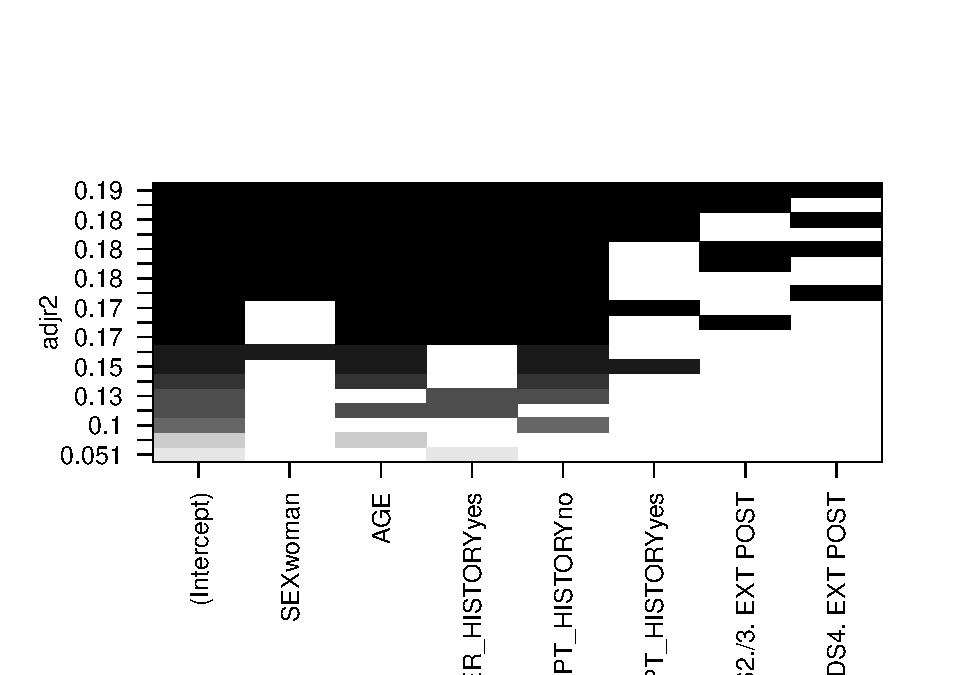
\includegraphics{Nexttry_files/figure-latex/unnamed-chunk-2-26.pdf}

\begin{Shaded}
\begin{Highlighting}[]
\CommentTok{\# First: AGE + SUIC\_ATTEMPT\_HISTORY (no):}
\NormalTok{besttwowithfirst}\OtherTok{\textless{}{-}}\FunctionTok{lm}\NormalTok{(ANXIETY\_STATE}\SpecialCharTok{\textasciitilde{}}\NormalTok{AGE}\SpecialCharTok{+}\NormalTok{SUIC\_ATTEMPT\_HISTORY,}\AttributeTok{data=}\NormalTok{table)}
\NormalTok{besttwowithfirst}
\end{Highlighting}
\end{Shaded}

\begin{verbatim}
## 
## Call:
## lm(formula = ANXIETY_STATE ~ AGE + SUIC_ATTEMPT_HISTORY, data = table)
## 
## Coefficients:
##             (Intercept)                      AGE   SUIC_ATTEMPT_HISTORYno  
##                 44.0587                  -0.2405                  -7.5820  
## SUIC_ATTEMPT_HISTORYyes  
##                  5.9432
\end{verbatim}

\begin{Shaded}
\begin{Highlighting}[]
\FunctionTok{summary}\NormalTok{(besttwowithfirst)}
\end{Highlighting}
\end{Shaded}

\begin{verbatim}
## 
## Call:
## lm(formula = ANXIETY_STATE ~ AGE + SUIC_ATTEMPT_HISTORY, data = table)
## 
## Residuals:
##     Min      1Q  Median      3Q     Max 
## -42.268  -9.771  -0.901   9.696  37.106 
## 
## Coefficients:
##                         Estimate Std. Error t value Pr(>|t|)    
## (Intercept)             44.05869    1.24696  35.333  < 2e-16 ***
## AGE                     -0.24051    0.03498  -6.875 1.04e-11 ***
## SUIC_ATTEMPT_HISTORYno  -7.58203    0.94939  -7.986 3.50e-15 ***
## SUIC_ATTEMPT_HISTORYyes  5.94320    1.76405   3.369  0.00078 ***
## ---
## Signif. codes:  0 '***' 0.001 '**' 0.01 '*' 0.05 '.' 0.1 ' ' 1
## 
## Residual standard error: 13.37 on 1096 degrees of freedom
## Multiple R-squared:  0.1489, Adjusted R-squared:  0.1466 
## F-statistic: 63.92 on 3 and 1096 DF,  p-value: < 2.2e-16
\end{verbatim}

\begin{Shaded}
\begin{Highlighting}[]
\FunctionTok{confint}\NormalTok{(besttwowithfirst)}
\end{Highlighting}
\end{Shaded}

\begin{verbatim}
##                              2.5 %     97.5 %
## (Intercept)             41.6119969 46.5053777
## AGE                     -0.3091526 -0.1718685
## SUIC_ATTEMPT_HISTORYno  -9.4448518 -5.7192060
## SUIC_ATTEMPT_HISTORYyes  2.4819007  9.4044902
\end{verbatim}

\begin{Shaded}
\begin{Highlighting}[]
\CommentTok{\# Second: MENTAL DISORDER (yes) + SUIC\_ATTEMPT\_HISTORY (no):}
\NormalTok{besttwowithsecond}\OtherTok{\textless{}{-}}\FunctionTok{lm}\NormalTok{(ANXIETY\_STATE}\SpecialCharTok{\textasciitilde{}}\NormalTok{MENTAL\_DISORDER\_HISTORY}\SpecialCharTok{+}\NormalTok{SUIC\_ATTEMPT\_HISTORY,}\AttributeTok{data=}\NormalTok{table)}
\NormalTok{besttwowithsecond}
\end{Highlighting}
\end{Shaded}

\begin{verbatim}
## 
## Call:
## lm(formula = ANXIETY_STATE ~ MENTAL_DISORDER_HISTORY + SUIC_ATTEMPT_HISTORY, 
##     data = table)
## 
## Coefficients:
##                (Intercept)  MENTAL_DISORDER_HISTORYyes  
##                     35.507                       4.862  
##     SUIC_ATTEMPT_HISTORYno     SUIC_ATTEMPT_HISTORYyes  
##                     -7.925                       4.490
\end{verbatim}

\begin{Shaded}
\begin{Highlighting}[]
\FunctionTok{summary}\NormalTok{(besttwowithsecond)}
\end{Highlighting}
\end{Shaded}

\begin{verbatim}
## 
## Call:
## lm(formula = ANXIETY_STATE ~ MENTAL_DISORDER_HISTORY + SUIC_ATTEMPT_HISTORY, 
##     data = table)
## 
## Residuals:
##     Min      1Q  Median      3Q     Max 
## -39.370  -9.582  -0.407   9.630  37.418 
## 
## Coefficients:
##                            Estimate Std. Error t value Pr(>|t|)    
## (Intercept)                 35.5072     0.8805  40.325  < 2e-16 ***
## MENTAL_DISORDER_HISTORYyes   4.8624     0.9524   5.105 3.90e-07 ***
## SUIC_ATTEMPT_HISTORYno      -7.9248     0.9579  -8.273 3.75e-16 ***
## SUIC_ATTEMPT_HISTORYyes      4.4898     1.7881   2.511   0.0122 *  
## ---
## Signif. codes:  0 '***' 0.001 '**' 0.01 '*' 0.05 '.' 0.1 ' ' 1
## 
## Residual standard error: 13.5 on 1096 degrees of freedom
## Multiple R-squared:  0.1328, Adjusted R-squared:  0.1305 
## F-statistic: 55.96 on 3 and 1096 DF,  p-value: < 2.2e-16
\end{verbatim}

\begin{Shaded}
\begin{Highlighting}[]
\FunctionTok{confint}\NormalTok{(besttwowithsecond)}
\end{Highlighting}
\end{Shaded}

\begin{verbatim}
##                                 2.5 %    97.5 %
## (Intercept)                33.7794670 37.234841
## MENTAL_DISORDER_HISTORYyes  2.9935400  6.731182
## SUIC_ATTEMPT_HISTORYno     -9.8042751 -6.045270
## SUIC_ATTEMPT_HISTORYyes     0.9813743  7.998230
\end{verbatim}

\begin{Shaded}
\begin{Highlighting}[]
\CommentTok{\# Third: AGE + MENTAL DISORDER (yes):}
\NormalTok{besttwowiththird}\OtherTok{\textless{}{-}}\FunctionTok{lm}\NormalTok{(ANXIETY\_STATE}\SpecialCharTok{\textasciitilde{}}\NormalTok{AGE}\SpecialCharTok{+}\NormalTok{MENTAL\_DISORDER\_HISTORY,}\AttributeTok{data=}\NormalTok{table)}
\NormalTok{besttwowiththird}
\end{Highlighting}
\end{Shaded}

\begin{verbatim}
## 
## Call:
## lm(formula = ANXIETY_STATE ~ AGE + MENTAL_DISORDER_HISTORY, data = table)
## 
## Coefficients:
##                (Intercept)                         AGE  
##                    39.8532                     -0.3256  
## MENTAL_DISORDER_HISTORYyes  
##                     8.0116
\end{verbatim}

\begin{Shaded}
\begin{Highlighting}[]
\FunctionTok{summary}\NormalTok{(besttwowiththird)}
\end{Highlighting}
\end{Shaded}

\begin{verbatim}
## 
## Call:
## lm(formula = ANXIETY_STATE ~ AGE + MENTAL_DISORDER_HISTORY, data = table)
## 
## Residuals:
##     Min      1Q  Median      3Q     Max 
## -40.678 -10.088  -0.981  10.220  36.543 
## 
## Coefficients:
##                            Estimate Std. Error t value Pr(>|t|)    
## (Intercept)                39.85323    1.18056  33.758   <2e-16 ***
## AGE                        -0.32560    0.03482  -9.351   <2e-16 ***
## MENTAL_DISORDER_HISTORYyes  8.01157    0.92369   8.673   <2e-16 ***
## ---
## Signif. codes:  0 '***' 0.001 '**' 0.01 '*' 0.05 '.' 0.1 ' ' 1
## 
## Residual standard error: 13.57 on 1097 degrees of freedom
## Multiple R-squared:  0.1223, Adjusted R-squared:  0.1207 
## F-statistic:  76.4 on 2 and 1097 DF,  p-value: < 2.2e-16
\end{verbatim}

\begin{Shaded}
\begin{Highlighting}[]
\FunctionTok{confint}\NormalTok{(besttwowiththird)}
\end{Highlighting}
\end{Shaded}

\begin{verbatim}
##                                 2.5 %     97.5 %
## (Intercept)                37.5368184 42.1696497
## AGE                        -0.3939187 -0.2572746
## MENTAL_DISORDER_HISTORYyes  6.1991683  9.8239651
\end{verbatim}

\begin{Shaded}
\begin{Highlighting}[]
\DocumentationTok{\#\#\#\# ANXIETY{-}TRAIT:}
\CommentTok{\# Stepwise Regression}
\NormalTok{fitwith}\OtherTok{\textless{}{-}}\FunctionTok{lm}\NormalTok{(ANXIETY\_TRAIT}\SpecialCharTok{\textasciitilde{}}\NormalTok{SEX}\SpecialCharTok{+}\NormalTok{AGE}\SpecialCharTok{+}\NormalTok{PROVINCE}\SpecialCharTok{+}\NormalTok{EDUCATION}\SpecialCharTok{+}\NormalTok{ECONOMIC\_INCOME}\SpecialCharTok{+}\NormalTok{LIVING\_WITH\_SOMEBODY}\SpecialCharTok{+}\NormalTok{MENTAL\_DISORDER\_HISTORY}\SpecialCharTok{+}\NormalTok{SUIC\_ATTEMPT\_HISTORY}\SpecialCharTok{+}\NormalTok{SUB\_PERIODS,}\AttributeTok{data=}\NormalTok{table)}
\NormalTok{stepwith }\OtherTok{\textless{}{-}} \FunctionTok{stepAIC}\NormalTok{(fitwith, }\AttributeTok{trace=}\ConstantTok{TRUE}\NormalTok{,}\AttributeTok{direction=}\StringTok{"both"}\NormalTok{)}
\end{Highlighting}
\end{Shaded}

\begin{verbatim}
## Start:  AIC=5137.82
## ANXIETY_TRAIT ~ SEX + AGE + PROVINCE + EDUCATION + ECONOMIC_INCOME + 
##     LIVING_WITH_SOMEBODY + MENTAL_DISORDER_HISTORY + SUIC_ATTEMPT_HISTORY + 
##     SUB_PERIODS
## 
##                           Df Sum of Sq    RSS    AIC
## - EDUCATION                8     935.0 109557 5131.2
## - PROVINCE                25    4675.0 113297 5134.2
## - SUB_PERIODS              2     137.9 108760 5135.2
## - LIVING_WITH_SOMEBODY     1      13.3 108635 5136.0
## <none>                                 108622 5137.8
## - ECONOMIC_INCOME          1     264.8 108887 5138.5
## - SEX                      1    2816.4 111438 5164.0
## - AGE                      1    4944.6 113567 5184.8
## - MENTAL_DISORDER_HISTORY  1    5600.0 114222 5191.1
## - SUIC_ATTEMPT_HISTORY     2   12682.4 121304 5255.3
## 
## Step:  AIC=5131.25
## ANXIETY_TRAIT ~ SEX + AGE + PROVINCE + ECONOMIC_INCOME + LIVING_WITH_SOMEBODY + 
##     MENTAL_DISORDER_HISTORY + SUIC_ATTEMPT_HISTORY + SUB_PERIODS
## 
##                           Df Sum of Sq    RSS    AIC
## - PROVINCE                25    4557.7 114115 5126.1
## - SUB_PERIODS              2     189.0 109746 5129.1
## - LIVING_WITH_SOMEBODY     1      16.3 109573 5129.4
## <none>                                 109557 5131.2
## - ECONOMIC_INCOME          1     329.8 109887 5132.6
## + EDUCATION                8     935.0 108622 5137.8
## - SEX                      1    2861.4 112418 5157.6
## - MENTAL_DISORDER_HISTORY  1    5490.9 115048 5183.0
## - AGE                      1    6186.4 115743 5189.7
## - SUIC_ATTEMPT_HISTORY     2   13466.8 123024 5254.8
## 
## Step:  AIC=5126.08
## ANXIETY_TRAIT ~ SEX + AGE + ECONOMIC_INCOME + LIVING_WITH_SOMEBODY + 
##     MENTAL_DISORDER_HISTORY + SUIC_ATTEMPT_HISTORY + SUB_PERIODS
## 
##                           Df Sum of Sq    RSS    AIC
## - LIVING_WITH_SOMEBODY     1      65.3 114180 5124.7
## - SUB_PERIODS              2     341.7 114456 5125.4
## <none>                                 114115 5126.1
## - ECONOMIC_INCOME          1     377.4 114492 5127.7
## + PROVINCE                25    4557.7 109557 5131.2
## + EDUCATION                8     817.7 113297 5134.2
## - SEX                      1    2828.0 116943 5151.0
## - MENTAL_DISORDER_HISTORY  1    5899.9 120015 5179.5
## - AGE                      1    6523.8 120638 5185.2
## - SUIC_ATTEMPT_HISTORY     2   14577.2 128692 5254.3
## 
## Step:  AIC=5124.71
## ANXIETY_TRAIT ~ SEX + AGE + ECONOMIC_INCOME + MENTAL_DISORDER_HISTORY + 
##     SUIC_ATTEMPT_HISTORY + SUB_PERIODS
## 
##                           Df Sum of Sq    RSS    AIC
## - SUB_PERIODS              2     333.1 114513 5123.9
## <none>                                 114180 5124.7
## + LIVING_WITH_SOMEBODY     1      65.3 114115 5126.1
## - ECONOMIC_INCOME          1     359.5 114540 5126.2
## + PROVINCE                25    4606.7 109573 5129.4
## + EDUCATION                8     828.7 113351 5132.7
## - SEX                      1    2782.3 116962 5149.2
## - MENTAL_DISORDER_HISTORY  1    6011.6 120192 5179.2
## - AGE                      1    6467.2 120647 5183.3
## - SUIC_ATTEMPT_HISTORY     2   14651.3 128831 5253.5
## 
## Step:  AIC=5123.92
## ANXIETY_TRAIT ~ SEX + AGE + ECONOMIC_INCOME + MENTAL_DISORDER_HISTORY + 
##     SUIC_ATTEMPT_HISTORY
## 
##                           Df Sum of Sq    RSS    AIC
## <none>                                 114513 5123.9
## + SUB_PERIODS              2     333.1 114180 5124.7
## - ECONOMIC_INCOME          1     350.5 114864 5125.3
## + LIVING_WITH_SOMEBODY     1      56.8 114456 5125.4
## + PROVINCE                25    4752.4 109761 5127.3
## + EDUCATION                8     844.3 113669 5131.8
## - SEX                      1    2775.3 117289 5148.3
## - MENTAL_DISORDER_HISTORY  1    6068.6 120582 5178.7
## - AGE                      1    7369.5 121883 5190.5
## - SUIC_ATTEMPT_HISTORY     2   14718.2 129231 5252.9
\end{verbatim}

\begin{Shaded}
\begin{Highlighting}[]
\NormalTok{stepwith}
\end{Highlighting}
\end{Shaded}

\begin{verbatim}
## 
## Call:
## lm(formula = ANXIETY_TRAIT ~ SEX + AGE + ECONOMIC_INCOME + MENTAL_DISORDER_HISTORY + 
##     SUIC_ATTEMPT_HISTORY, data = table)
## 
## Coefficients:
##                (Intercept)                    SEXwoman  
##                    35.5481                      4.0265  
##                        AGE          ECONOMIC_INCOMEyes  
##                    -0.2293                     -1.5578  
## MENTAL_DISORDER_HISTORYyes      SUIC_ATTEMPT_HISTORYno  
##                     5.5442                     -7.5304  
##    SUIC_ATTEMPT_HISTORYyes  
##                     3.2393
\end{verbatim}

\begin{Shaded}
\begin{Highlighting}[]
\NormalTok{stepwith}\SpecialCharTok{$}\NormalTok{anova }\CommentTok{\# display results}
\end{Highlighting}
\end{Shaded}

\begin{verbatim}
## Stepwise Model Path 
## Analysis of Deviance Table
## 
## Initial Model:
## ANXIETY_TRAIT ~ SEX + AGE + PROVINCE + EDUCATION + ECONOMIC_INCOME + 
##     LIVING_WITH_SOMEBODY + MENTAL_DISORDER_HISTORY + SUIC_ATTEMPT_HISTORY + 
##     SUB_PERIODS
## 
## Final Model:
## ANXIETY_TRAIT ~ SEX + AGE + ECONOMIC_INCOME + MENTAL_DISORDER_HISTORY + 
##     SUIC_ATTEMPT_HISTORY
## 
## 
##                     Step Df   Deviance Resid. Df Resid. Dev      AIC
## 1                                           1057   108622.1 5137.821
## 2            - EDUCATION  8  934.97893      1065   109557.0 5131.249
## 3             - PROVINCE 25 4557.68671      1090   114114.7 5126.084
## 4 - LIVING_WITH_SOMEBODY  1   65.30652      1091   114180.0 5124.713
## 5          - SUB_PERIODS  2  333.13652      1093   114513.2 5123.918
\end{verbatim}

\begin{Shaded}
\begin{Highlighting}[]
\CommentTok{\# Stepwise Model Path }
\CommentTok{\# Analysis of Deviance Table}
\CommentTok{\# Initial Model: ANXIETY\_TRAIT \textasciitilde{} SEX + AGE + PROVINCE + EDUCATION + ECONOMIC\_INCOME + LIVING\_WITH\_SOMEBODY + MENTAL\_DISORDER\_HISTORY + SUIC\_ATTEMPT\_HISTORY + SUB\_PERIODS}
\CommentTok{\# Start:  AIC = 5137.82}
\CommentTok{\# Final Model: ANXIETY\_TRAIT \textasciitilde{} SEX + AGE + ECONOMIC\_INCOME + MENTAL\_DISORDER\_HISTORY + SUIC\_ATTEMPT\_HISTORY}
\CommentTok{\# Stepwith:  AIC = 5123.92}
\FunctionTok{summary}\NormalTok{(stepwith)}
\end{Highlighting}
\end{Shaded}

\begin{verbatim}
## 
## Call:
## lm(formula = ANXIETY_TRAIT ~ SEX + AGE + ECONOMIC_INCOME + MENTAL_DISORDER_HISTORY + 
##     SUIC_ATTEMPT_HISTORY, data = table)
## 
## Residuals:
##     Min      1Q  Median      3Q     Max 
## -34.532  -6.984  -0.446   7.335  30.631 
## 
## Coefficients:
##                            Estimate Std. Error t value Pr(>|t|)    
## (Intercept)                35.54809    1.33510  26.626  < 2e-16 ***
## SEXwoman                    4.02646    0.78232   5.147 3.14e-07 ***
## AGE                        -0.22934    0.02735  -8.387  < 2e-16 ***
## ECONOMIC_INCOMEyes         -1.55779    0.85164  -1.829   0.0676 .  
## MENTAL_DISORDER_HISTORYyes  5.54423    0.72847   7.611 5.87e-14 ***
## SUIC_ATTEMPT_HISTORYno     -7.53035    0.74687 -10.083  < 2e-16 ***
## SUIC_ATTEMPT_HISTORYyes     3.23926    1.35869   2.384   0.0173 *  
## ---
## Signif. codes:  0 '***' 0.001 '**' 0.01 '*' 0.05 '.' 0.1 ' ' 1
## 
## Residual standard error: 10.24 on 1093 degrees of freedom
## Multiple R-squared:  0.2939, Adjusted R-squared:   0.29 
## F-statistic: 75.83 on 6 and 1093 DF,  p-value: < 2.2e-16
\end{verbatim}

\begin{Shaded}
\begin{Highlighting}[]
\CommentTok{\# 95\% Confidence interval of best{-}fitted model:}
\FunctionTok{confint}\NormalTok{(stepwith)}
\end{Highlighting}
\end{Shaded}

\begin{verbatim}
##                                 2.5 %     97.5 %
## (Intercept)                32.9284370 38.1677508
## SEXwoman                    2.4914440  5.5614758
## AGE                        -0.2830004 -0.1756886
## ECONOMIC_INCOMEyes         -3.2288274  0.1132542
## MENTAL_DISORDER_HISTORYyes  4.1148672  6.9735910
## SUIC_ATTEMPT_HISTORYno     -8.9958149 -6.0648884
## SUIC_ATTEMPT_HISTORYyes     0.5733268  5.9052013
\end{verbatim}

\begin{Shaded}
\begin{Highlighting}[]
\CommentTok{\# ERROR RATE of best{-}fitted model:}
\FunctionTok{sigma}\NormalTok{(stepwith)}\SpecialCharTok{/}\FunctionTok{mean}\NormalTok{(table}\SpecialCharTok{$}\NormalTok{ANXIETY\_TRAIT)}
\end{Highlighting}
\end{Shaded}

\begin{verbatim}
## [1] 0.380548
\end{verbatim}

\begin{Shaded}
\begin{Highlighting}[]
\CommentTok{\# 0.380548}
\CommentTok{\# In our multiple regression example, the Residual Standard Error (RSE) or sigma is 10.24 corresponding to 38\% error rate.}

\FunctionTok{par}\NormalTok{(}\AttributeTok{mfrow=}\FunctionTok{c}\NormalTok{(}\DecValTok{2}\NormalTok{,}\DecValTok{2}\NormalTok{))}
\CommentTok{\# Figure S7 (Supplementary material)}
\FunctionTok{plot}\NormalTok{(stepwith)}
\end{Highlighting}
\end{Shaded}

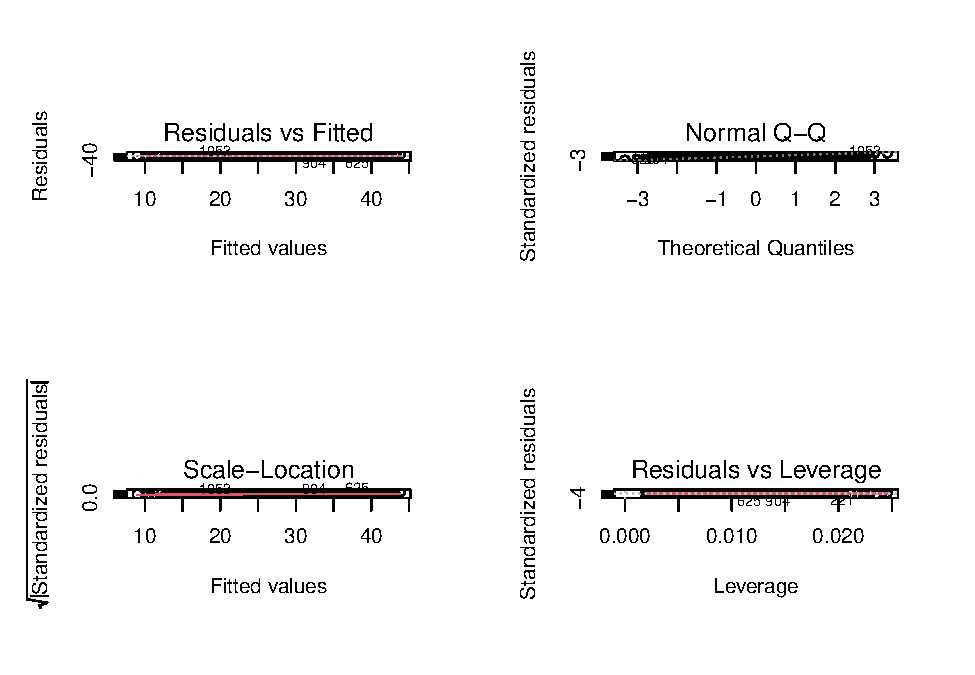
\includegraphics{Nexttry_files/figure-latex/unnamed-chunk-2-27.pdf}

\begin{Shaded}
\begin{Highlighting}[]
\FunctionTok{par}\NormalTok{(}\AttributeTok{mfrow=}\FunctionTok{c}\NormalTok{(}\DecValTok{1}\NormalTok{,}\DecValTok{1}\NormalTok{))}



\CommentTok{\# TABLE 1:}

\CommentTok{\# Model 1: INITIAL MODEL:}
\NormalTok{model1}\OtherTok{\textless{}{-}}\FunctionTok{lm}\NormalTok{(ANXIETY\_TRAIT}\SpecialCharTok{\textasciitilde{}}\NormalTok{SEX}\SpecialCharTok{+}\NormalTok{AGE}\SpecialCharTok{+}\NormalTok{PROVINCE}\SpecialCharTok{+}\NormalTok{EDUCATION}\SpecialCharTok{+}\NormalTok{ECONOMIC\_INCOME}\SpecialCharTok{+}\NormalTok{LIVING\_WITH\_SOMEBODY}\SpecialCharTok{+}\NormalTok{MENTAL\_DISORDER\_HISTORY}\SpecialCharTok{+}\NormalTok{SUIC\_ATTEMPT\_HISTORY}\SpecialCharTok{+}\NormalTok{SUB\_PERIODS,}\AttributeTok{data=}\NormalTok{table)}
\FunctionTok{summary}\NormalTok{(model1)}
\end{Highlighting}
\end{Shaded}

\begin{verbatim}
## 
## Call:
## lm(formula = ANXIETY_TRAIT ~ SEX + AGE + PROVINCE + EDUCATION + 
##     ECONOMIC_INCOME + LIVING_WITH_SOMEBODY + MENTAL_DISORDER_HISTORY + 
##     SUIC_ATTEMPT_HISTORY + SUB_PERIODS, data = table)
## 
## Residuals:
##     Min      1Q  Median      3Q     Max 
## -34.310  -6.814  -0.099   6.682  30.083 
## 
## Coefficients:
##                                             Estimate Std. Error t value
## (Intercept)                                 24.57072    7.47927   3.285
## SEXwoman                                     4.18407    0.79923   5.235
## AGE                                         -0.21745    0.03135  -6.937
## PROVINCECABA (Buenos Aires capital)         -0.01606    1.24464  -0.013
## PROVINCECatamarca                            9.13782    7.33729   1.245
## PROVINCEChaco                               -5.05123    3.92776  -1.286
## PROVINCEChubut                              -0.27607    5.14099  -0.054
## PROVINCECórdoba                             -3.06623    0.96304  -3.184
## PROVINCECorrientes                         -10.23225    4.61152  -2.219
## PROVINCEEntre Ríos                          -1.37982    2.74880  -0.502
## PROVINCEFormosa                             -0.34612    5.92624  -0.058
## PROVINCEJujuy                               -0.14799    1.89486  -0.078
## PROVINCELa Pampa                            -7.54914    3.67923  -2.052
## PROVINCELa Rioja                           -10.75603   10.23462  -1.051
## PROVINCEMendoza                              4.39400    2.59330   1.694
## PROVINCEMisiones                            -7.38321    2.81880  -2.619
## PROVINCENeuquén                             -6.76139    3.56813  -1.895
## PROVINCEother                               -2.03408    2.53966  -0.801
## PROVINCEOtro                                 7.55244    5.98580   1.262
## PROVINCERío Negro                           -0.37854    5.14259  -0.074
## PROVINCESalta                                2.70002    3.03563   0.889
## PROVINCESan Juan                            -3.55480    5.17556  -0.687
## PROVINCESan Luis                            14.85952   10.22449   1.453
## PROVINCESanta Cruz                           3.74716    7.23202   0.518
## PROVINCESanta Fe                            -2.33938    0.95773  -2.443
## PROVINCESantiago del Estero                 -1.31744    2.82011  -0.467
## PROVINCETierra del Fuego                    -0.99563    2.46287  -0.404
## PROVINCETucumán                             -1.53539    2.15079  -0.714
## EDUCATIONCompleted high school              12.19140    7.30860   1.668
## EDUCATIONCompleted postgraduate             11.24984    7.30777   1.539
## EDUCATIONCompleted tertiary or university   10.66463    7.27292   1.466
## EDUCATIONIncomplete elementary school       12.33674   12.49045   0.988
## EDUCATIONIncomplete high school             15.16058    7.54845   2.008
## EDUCATIONIncomplete postgraduate            12.20045    7.33684   1.663
## EDUCATIONIncomplete tertiary or university  11.59027    7.26461   1.595
## EDUCATIONOtro                               18.91489   10.36495   1.825
## ECONOMIC_INCOMEyes                          -1.39494    0.86897  -1.605
## LIVING_WITH_SOMEBODYyes                     -0.32343    0.89986  -0.359
## MENTAL_DISORDER_HISTORYyes                   5.41671    0.73378   7.382
## SUIC_ATTEMPT_HISTORYno                      -7.18724    0.75780  -9.484
## SUIC_ATTEMPT_HISTORYyes                      3.10419    1.36316   2.277
## SUB_PERIODS2./3. EXT POST                    0.61700    0.90511   0.682
## SUB_PERIODS4. EXT POST                       0.95866    0.83610   1.147
##                                            Pr(>|t|)    
## (Intercept)                                 0.00105 ** 
## SEXwoman                                   1.99e-07 ***
## AGE                                        6.99e-12 ***
## PROVINCECABA (Buenos Aires capital)         0.98971    
## PROVINCECatamarca                           0.21326    
## PROVINCEChaco                               0.19871    
## PROVINCEChubut                              0.95718    
## PROVINCECórdoba                             0.00150 ** 
## PROVINCECorrientes                          0.02671 *  
## PROVINCEEntre Ríos                          0.61579    
## PROVINCEFormosa                             0.95344    
## PROVINCEJujuy                               0.93776    
## PROVINCELa Pampa                            0.04043 *  
## PROVINCELa Rioja                            0.29352    
## PROVINCEMendoza                             0.09049 .  
## PROVINCEMisiones                            0.00894 ** 
## PROVINCENeuquén                             0.05837 .  
## PROVINCEother                               0.42335    
## PROVINCEOtro                                0.20733    
## PROVINCERío Negro                           0.94134    
## PROVINCESalta                               0.37397    
## PROVINCESan Juan                            0.49233    
## PROVINCESan Luis                            0.14643    
## PROVINCESanta Cruz                          0.60447    
## PROVINCESanta Fe                            0.01474 *  
## PROVINCESantiago del Estero                 0.64048    
## PROVINCETierra del Fuego                    0.68611    
## PROVINCETucumán                             0.47547    
## EDUCATIONCompleted high school              0.09559 .  
## EDUCATIONCompleted postgraduate             0.12400    
## EDUCATIONCompleted tertiary or university   0.14285    
## EDUCATIONIncomplete elementary school       0.32353    
## EDUCATIONIncomplete high school             0.04485 *  
## EDUCATIONIncomplete postgraduate            0.09663 .  
## EDUCATIONIncomplete tertiary or university  0.11091    
## EDUCATIONOtro                               0.06830 .  
## ECONOMIC_INCOMEyes                          0.10873    
## LIVING_WITH_SOMEBODYyes                     0.71935    
## MENTAL_DISORDER_HISTORYyes                 3.15e-13 ***
## SUIC_ATTEMPT_HISTORYno                      < 2e-16 ***
## SUIC_ATTEMPT_HISTORYyes                     0.02297 *  
## SUB_PERIODS2./3. EXT POST                   0.49559    
## SUB_PERIODS4. EXT POST                      0.25181    
## ---
## Signif. codes:  0 '***' 0.001 '**' 0.01 '*' 0.05 '.' 0.1 ' ' 1
## 
## Residual standard error: 10.14 on 1057 degrees of freedom
## Multiple R-squared:  0.3302, Adjusted R-squared:  0.3036 
## F-statistic: 12.41 on 42 and 1057 DF,  p-value: < 2.2e-16
\end{verbatim}

\begin{Shaded}
\begin{Highlighting}[]
\CommentTok{\# YES significative p{-}value \textless{} 2.2e{-}16}

\CommentTok{\# Model 2 eliminates EDUCATION:}
\NormalTok{model2}\OtherTok{\textless{}{-}}\FunctionTok{lm}\NormalTok{(ANXIETY\_TRAIT}\SpecialCharTok{\textasciitilde{}}\NormalTok{SEX}\SpecialCharTok{+}\NormalTok{AGE}\SpecialCharTok{+}\NormalTok{PROVINCE}\SpecialCharTok{+}\NormalTok{ECONOMIC\_INCOME}\SpecialCharTok{+}\NormalTok{LIVING\_WITH\_SOMEBODY}\SpecialCharTok{+}\NormalTok{MENTAL\_DISORDER\_HISTORY}\SpecialCharTok{+}\NormalTok{SUIC\_ATTEMPT\_HISTORY}\SpecialCharTok{+}\NormalTok{SUB\_PERIODS,}\AttributeTok{data=}\NormalTok{table)}
\FunctionTok{summary}\NormalTok{(model2)}
\end{Highlighting}
\end{Shaded}

\begin{verbatim}
## 
## Call:
## lm(formula = ANXIETY_TRAIT ~ SEX + AGE + PROVINCE + ECONOMIC_INCOME + 
##     LIVING_WITH_SOMEBODY + MENTAL_DISORDER_HISTORY + SUIC_ATTEMPT_HISTORY + 
##     SUB_PERIODS, data = table)
## 
## Residuals:
##     Min      1Q  Median      3Q     Max 
## -33.795  -6.986  -0.155   6.766  31.020 
## 
## Coefficients:
##                                      Estimate Std. Error t value Pr(>|t|)    
## (Intercept)                          36.47419    1.82396  19.997  < 2e-16 ***
## SEXwoman                              4.20073    0.79649   5.274 1.62e-07 ***
## AGE                                  -0.22752    0.02934  -7.755 2.06e-14 ***
## PROVINCECABA (Buenos Aires capital)  -0.03075    1.24000  -0.025  0.98022    
## PROVINCECatamarca                    10.90091    7.25566   1.502  0.13329    
## PROVINCEChaco                        -5.24591    3.92072  -1.338  0.18118    
## PROVINCEChubut                       -0.54530    5.13491  -0.106  0.91545    
## PROVINCECórdoba                      -2.89134    0.95339  -3.033  0.00248 ** 
## PROVINCECorrientes                  -10.25121    4.60943  -2.224  0.02636 *  
## PROVINCEEntre Ríos                   -1.44658    2.74765  -0.526  0.59867    
## PROVINCEFormosa                      -0.21821    5.92407  -0.037  0.97062    
## PROVINCEJujuy                        -0.27622    1.89239  -0.146  0.88398    
## PROVINCELa Pampa                     -7.41166    3.67328  -2.018  0.04387 *  
## PROVINCELa Rioja                    -10.69663   10.20897  -1.048  0.29498    
## PROVINCEMendoza                       4.35817    2.57106   1.695  0.09035 .  
## PROVINCEMisiones                     -7.10783    2.80529  -2.534  0.01143 *  
## PROVINCENeuquén                      -6.17122    3.45840  -1.784  0.07464 .  
## PROVINCEother                        -2.00309    2.52024  -0.795  0.42691    
## PROVINCEOtro                          7.62988    5.95824   1.281  0.20063    
## PROVINCERío Negro                    -0.87342    5.13610  -0.170  0.86500    
## PROVINCESalta                         2.57174    3.03283   0.848  0.39665    
## PROVINCESan Juan                     -2.85902    5.13175  -0.557  0.57756    
## PROVINCESan Luis                     14.77687   10.18479   1.451  0.14711    
## PROVINCESanta Cruz                    3.66598    7.22865   0.507  0.61216    
## PROVINCESanta Fe                     -2.42314    0.95358  -2.541  0.01119 *  
## PROVINCESantiago del Estero          -1.48657    2.81723  -0.528  0.59784    
## PROVINCETierra del Fuego             -0.76220    2.45012  -0.311  0.75579    
## PROVINCETucumán                      -1.57539    2.14744  -0.734  0.46335    
## ECONOMIC_INCOMEyes                   -1.52761    0.85314  -1.791  0.07365 .  
## LIVING_WITH_SOMEBODYyes              -0.35577    0.89508  -0.397  0.69110    
## MENTAL_DISORDER_HISTORYyes            5.33893    0.73076   7.306 5.39e-13 ***
## SUIC_ATTEMPT_HISTORYno               -7.28778    0.75005  -9.716  < 2e-16 ***
## SUIC_ATTEMPT_HISTORYyes               3.24151    1.35760   2.388  0.01713 *  
## SUB_PERIODS2./3. EXT POST             0.70645    0.90176   0.783  0.43356    
## SUB_PERIODS4. EXT POST                1.11055    0.82663   1.343  0.17941    
## ---
## Signif. codes:  0 '***' 0.001 '**' 0.01 '*' 0.05 '.' 0.1 ' ' 1
## 
## Residual standard error: 10.14 on 1065 degrees of freedom
## Multiple R-squared:  0.3245, Adjusted R-squared:  0.3029 
## F-statistic: 15.05 on 34 and 1065 DF,  p-value: < 2.2e-16
\end{verbatim}

\begin{Shaded}
\begin{Highlighting}[]
\CommentTok{\# YES significative p{-}value \textless{} 2.2e{-}16}

\CommentTok{\# Model 3 eliminates PROVINCE:}
\NormalTok{model3}\OtherTok{\textless{}{-}}\FunctionTok{lm}\NormalTok{(ANXIETY\_TRAIT}\SpecialCharTok{\textasciitilde{}}\NormalTok{SEX}\SpecialCharTok{+}\NormalTok{AGE}\SpecialCharTok{+}\NormalTok{ECONOMIC\_INCOME}\SpecialCharTok{+}\NormalTok{LIVING\_WITH\_SOMEBODY}\SpecialCharTok{+}\NormalTok{MENTAL\_DISORDER\_HISTORY}\SpecialCharTok{+}\NormalTok{SUIC\_ATTEMPT\_HISTORY}\SpecialCharTok{+}\NormalTok{SUB\_PERIODS,}\AttributeTok{data=}\NormalTok{table)}
\FunctionTok{summary}\NormalTok{(model3)}
\end{Highlighting}
\end{Shaded}

\begin{verbatim}
## 
## Call:
## lm(formula = ANXIETY_TRAIT ~ SEX + AGE + ECONOMIC_INCOME + LIVING_WITH_SOMEBODY + 
##     MENTAL_DISORDER_HISTORY + SUIC_ATTEMPT_HISTORY + SUB_PERIODS, 
##     data = table)
## 
## Residuals:
##     Min      1Q  Median      3Q     Max 
## -34.704  -7.046  -0.393   7.281  30.440 
## 
## Coefficients:
##                            Estimate Std. Error t value Pr(>|t|)    
## (Intercept)                35.25064    1.72869  20.392  < 2e-16 ***
## SEXwoman                    4.10021    0.78891   5.197 2.41e-07 ***
## AGE                        -0.22549    0.02857  -7.894 7.10e-15 ***
## ECONOMIC_INCOMEyes         -1.61984    0.85318  -1.899   0.0579 .  
## LIVING_WITH_SOMEBODYyes    -0.70082    0.88733  -0.790   0.4298    
## MENTAL_DISORDER_HISTORYyes  5.48159    0.73020   7.507 1.25e-13 ***
## SUIC_ATTEMPT_HISTORYno     -7.53069    0.74703 -10.081  < 2e-16 ***
## SUIC_ATTEMPT_HISTORYyes     3.15244    1.36028   2.317   0.0207 *  
## SUB_PERIODS2./3. EXT POST   1.37016    0.85564   1.601   0.1096    
## SUB_PERIODS4. EXT POST      1.08260    0.72890   1.485   0.1378    
## ---
## Signif. codes:  0 '***' 0.001 '**' 0.01 '*' 0.05 '.' 0.1 ' ' 1
## 
## Residual standard error: 10.23 on 1090 degrees of freedom
## Multiple R-squared:  0.2964, Adjusted R-squared:  0.2906 
## F-statistic: 51.01 on 9 and 1090 DF,  p-value: < 2.2e-16
\end{verbatim}

\begin{Shaded}
\begin{Highlighting}[]
\CommentTok{\# YES significative p{-}value \textless{} 2.2e{-}16}

\CommentTok{\# Model 4 eliminates LIVING\_WITH\_SOMEBODY:}
\NormalTok{model4}\OtherTok{\textless{}{-}}\FunctionTok{lm}\NormalTok{(ANXIETY\_TRAIT}\SpecialCharTok{\textasciitilde{}}\NormalTok{SEX}\SpecialCharTok{+}\NormalTok{AGE}\SpecialCharTok{+}\NormalTok{ECONOMIC\_INCOME}\SpecialCharTok{+}\NormalTok{MENTAL\_DISORDER\_HISTORY}\SpecialCharTok{+}\NormalTok{SUIC\_ATTEMPT\_HISTORY}\SpecialCharTok{+}\NormalTok{SUB\_PERIODS,}\AttributeTok{data=}\NormalTok{table)}
\FunctionTok{summary}\NormalTok{(model4)}
\end{Highlighting}
\end{Shaded}

\begin{verbatim}
## 
## Call:
## lm(formula = ANXIETY_TRAIT ~ SEX + AGE + ECONOMIC_INCOME + MENTAL_DISORDER_HISTORY + 
##     SUIC_ATTEMPT_HISTORY + SUB_PERIODS, data = table)
## 
## Residuals:
##     Min      1Q  Median      3Q     Max 
## -34.762  -7.075  -0.441   7.219  30.267 
## 
## Coefficients:
##                            Estimate Std. Error t value Pr(>|t|)    
## (Intercept)                34.55288    1.48563  23.258  < 2e-16 ***
## SEXwoman                    4.05741    0.78691   5.156 2.99e-07 ***
## AGE                        -0.22241    0.02829  -7.861 9.11e-15 ***
## ECONOMIC_INCOMEyes         -1.57790    0.85138  -1.853   0.0641 .  
## MENTAL_DISORDER_HISTORYyes  5.52061    0.72841   7.579 7.41e-14 ***
## SUIC_ATTEMPT_HISTORYno     -7.53460    0.74689 -10.088  < 2e-16 ***
## SUIC_ATTEMPT_HISTORYyes     3.19868    1.35879   2.354   0.0187 *  
## SUB_PERIODS2./3. EXT POST   1.34187    0.85474   1.570   0.1167    
## SUB_PERIODS4. EXT POST      1.07928    0.72876   1.481   0.1389    
## ---
## Signif. codes:  0 '***' 0.001 '**' 0.01 '*' 0.05 '.' 0.1 ' ' 1
## 
## Residual standard error: 10.23 on 1091 degrees of freedom
## Multiple R-squared:  0.296,  Adjusted R-squared:  0.2908 
## F-statistic: 57.33 on 8 and 1091 DF,  p-value: < 2.2e-16
\end{verbatim}

\begin{Shaded}
\begin{Highlighting}[]
\CommentTok{\# YES significative p{-}value \textless{} 2.2e{-}16}

\CommentTok{\# Model 5 eliminates SUB PERIODS:}
\NormalTok{model4}\OtherTok{\textless{}{-}}\FunctionTok{lm}\NormalTok{(ANXIETY\_TRAIT}\SpecialCharTok{\textasciitilde{}}\NormalTok{SEX}\SpecialCharTok{+}\NormalTok{AGE}\SpecialCharTok{+}\NormalTok{ECONOMIC\_INCOME}\SpecialCharTok{+}\NormalTok{MENTAL\_DISORDER\_HISTORY}\SpecialCharTok{+}\NormalTok{SUIC\_ATTEMPT\_HISTORY,}\AttributeTok{data=}\NormalTok{table)}
\FunctionTok{summary}\NormalTok{(model4)}
\end{Highlighting}
\end{Shaded}

\begin{verbatim}
## 
## Call:
## lm(formula = ANXIETY_TRAIT ~ SEX + AGE + ECONOMIC_INCOME + MENTAL_DISORDER_HISTORY + 
##     SUIC_ATTEMPT_HISTORY, data = table)
## 
## Residuals:
##     Min      1Q  Median      3Q     Max 
## -34.532  -6.984  -0.446   7.335  30.631 
## 
## Coefficients:
##                            Estimate Std. Error t value Pr(>|t|)    
## (Intercept)                35.54809    1.33510  26.626  < 2e-16 ***
## SEXwoman                    4.02646    0.78232   5.147 3.14e-07 ***
## AGE                        -0.22934    0.02735  -8.387  < 2e-16 ***
## ECONOMIC_INCOMEyes         -1.55779    0.85164  -1.829   0.0676 .  
## MENTAL_DISORDER_HISTORYyes  5.54423    0.72847   7.611 5.87e-14 ***
## SUIC_ATTEMPT_HISTORYno     -7.53035    0.74687 -10.083  < 2e-16 ***
## SUIC_ATTEMPT_HISTORYyes     3.23926    1.35869   2.384   0.0173 *  
## ---
## Signif. codes:  0 '***' 0.001 '**' 0.01 '*' 0.05 '.' 0.1 ' ' 1
## 
## Residual standard error: 10.24 on 1093 degrees of freedom
## Multiple R-squared:  0.2939, Adjusted R-squared:   0.29 
## F-statistic: 75.83 on 6 and 1093 DF,  p-value: < 2.2e-16
\end{verbatim}

\begin{Shaded}
\begin{Highlighting}[]
\CommentTok{\# YES significative p{-}value \textless{} 2.2e{-}16}




\DocumentationTok{\#\#\#\#\#\#\#\#\#\#\#\#\#\#\#\#}
\DocumentationTok{\#\# Considering the predictors included in the best{-}fitted model (i.e., stepwith) in this group, we analyzed the smallest possible linear model for each specific MHS indicator by means of all two{-}predictor combinations.  }
\CommentTok{\# We performed all{-}subsets regression using the regsubsets() function from the leaps package.}
\CommentTok{\# We analyzed the three best models for two{-}predictor subset sizes.}

\NormalTok{leapsbestwith}\OtherTok{\textless{}{-}}\FunctionTok{regsubsets}\NormalTok{(ANXIETY\_TRAIT}\SpecialCharTok{\textasciitilde{}}\NormalTok{SEX}\SpecialCharTok{+}\NormalTok{AGE}\SpecialCharTok{+}\NormalTok{ECONOMIC\_INCOME}\SpecialCharTok{+}\NormalTok{MENTAL\_DISORDER\_HISTORY}\SpecialCharTok{+}\NormalTok{SUIC\_ATTEMPT\_HISTORY,}\AttributeTok{data=}\NormalTok{table,}\AttributeTok{nbest=}\DecValTok{3}\NormalTok{)}
\FunctionTok{summary}\NormalTok{(leapsbestwith)}
\end{Highlighting}
\end{Shaded}

\begin{verbatim}
## Subset selection object
## Call: regsubsets.formula(ANXIETY_TRAIT ~ SEX + AGE + ECONOMIC_INCOME + 
##     MENTAL_DISORDER_HISTORY + SUIC_ATTEMPT_HISTORY, data = table, 
##     nbest = 3)
## 6 Variables  (and intercept)
##                            Forced in Forced out
## SEXwoman                       FALSE      FALSE
## AGE                            FALSE      FALSE
## ECONOMIC_INCOMEyes             FALSE      FALSE
## MENTAL_DISORDER_HISTORYyes     FALSE      FALSE
## SUIC_ATTEMPT_HISTORYno         FALSE      FALSE
## SUIC_ATTEMPT_HISTORYyes        FALSE      FALSE
## 3 subsets of each size up to 6
## Selection Algorithm: exhaustive
##          SEXwoman AGE ECONOMIC_INCOMEyes MENTAL_DISORDER_HISTORYyes
## 1  ( 1 ) " "      " " " "                " "                       
## 1  ( 2 ) " "      "*" " "                " "                       
## 1  ( 3 ) " "      " " " "                "*"                       
## 2  ( 1 ) " "      "*" " "                " "                       
## 2  ( 2 ) " "      " " " "                "*"                       
## 2  ( 3 ) "*"      " " " "                " "                       
## 3  ( 1 ) " "      "*" " "                "*"                       
## 3  ( 2 ) "*"      "*" " "                " "                       
## 3  ( 3 ) "*"      " " " "                "*"                       
## 4  ( 1 ) "*"      "*" " "                "*"                       
## 4  ( 2 ) " "      "*" " "                "*"                       
## 4  ( 3 ) " "      "*" "*"                "*"                       
## 5  ( 1 ) "*"      "*" " "                "*"                       
## 5  ( 2 ) "*"      "*" "*"                "*"                       
## 5  ( 3 ) " "      "*" "*"                "*"                       
## 6  ( 1 ) "*"      "*" "*"                "*"                       
##          SUIC_ATTEMPT_HISTORYno SUIC_ATTEMPT_HISTORYyes
## 1  ( 1 ) "*"                    " "                    
## 1  ( 2 ) " "                    " "                    
## 1  ( 3 ) " "                    " "                    
## 2  ( 1 ) "*"                    " "                    
## 2  ( 2 ) "*"                    " "                    
## 2  ( 3 ) "*"                    " "                    
## 3  ( 1 ) "*"                    " "                    
## 3  ( 2 ) "*"                    " "                    
## 3  ( 3 ) "*"                    " "                    
## 4  ( 1 ) "*"                    " "                    
## 4  ( 2 ) "*"                    "*"                    
## 4  ( 3 ) "*"                    " "                    
## 5  ( 1 ) "*"                    "*"                    
## 5  ( 2 ) "*"                    " "                    
## 5  ( 3 ) "*"                    "*"                    
## 6  ( 1 ) "*"                    "*"
\end{verbatim}

\begin{Shaded}
\begin{Highlighting}[]
\CommentTok{\# The best two{-}predictors model was: ANXIETY\_STATE \textasciitilde{} AGE + SUIC\_ATTEMPT\_HISTORY==no}

\FunctionTok{plot}\NormalTok{(leapsbestwith,}\AttributeTok{scale=}\StringTok{"r2"}\NormalTok{)}
\end{Highlighting}
\end{Shaded}

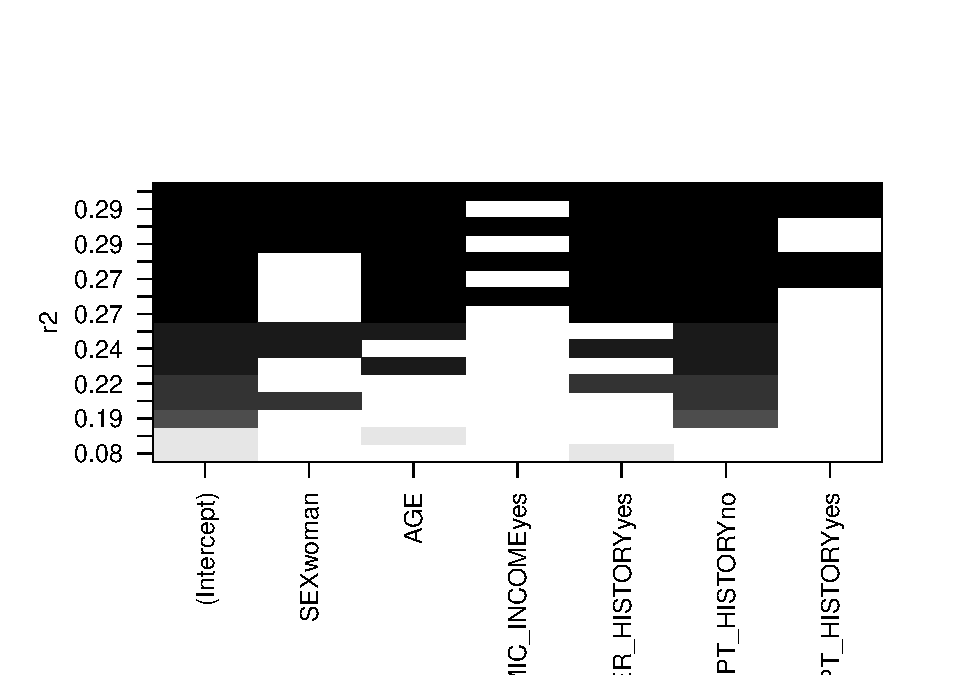
\includegraphics{Nexttry_files/figure-latex/unnamed-chunk-2-28.pdf}

\begin{Shaded}
\begin{Highlighting}[]
\FunctionTok{plot}\NormalTok{(leapsbestwith,}\AttributeTok{scale=}\StringTok{"adjr2"}\NormalTok{)}
\end{Highlighting}
\end{Shaded}

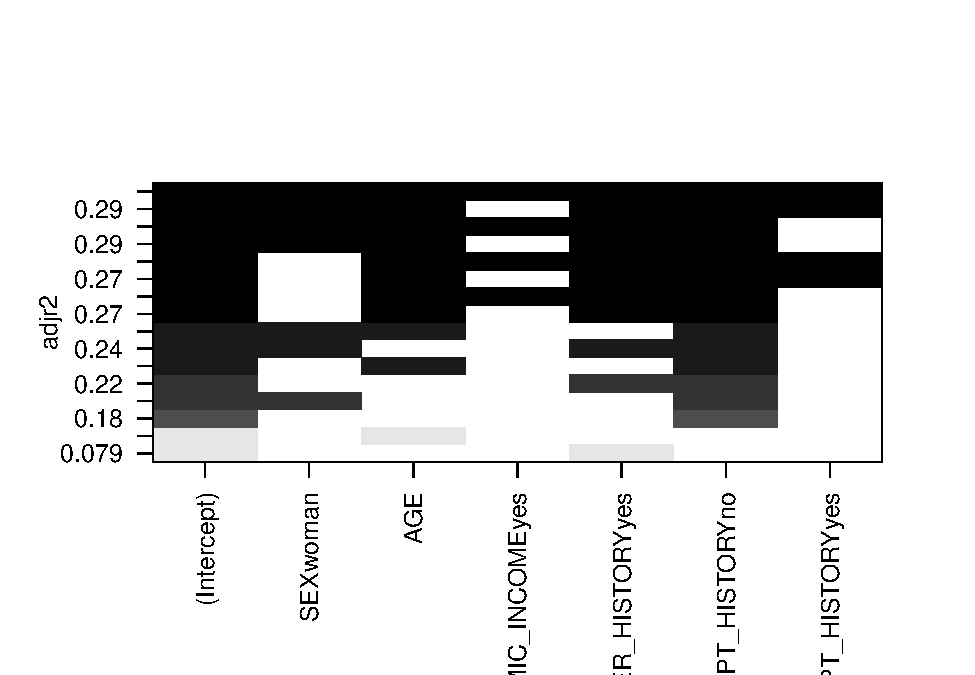
\includegraphics{Nexttry_files/figure-latex/unnamed-chunk-2-29.pdf}

\begin{Shaded}
\begin{Highlighting}[]
\CommentTok{\# First: AGE + SUIC\_ATTEMPT\_HISTORY (no):}
\NormalTok{besttwowithfirst}\OtherTok{\textless{}{-}}\FunctionTok{lm}\NormalTok{(ANXIETY\_TRAIT}\SpecialCharTok{\textasciitilde{}}\NormalTok{AGE}\SpecialCharTok{+}\NormalTok{SUIC\_ATTEMPT\_HISTORY,}\AttributeTok{data=}\NormalTok{table)}
\NormalTok{besttwowithfirst}
\end{Highlighting}
\end{Shaded}

\begin{verbatim}
## 
## Call:
## lm(formula = ANXIETY_TRAIT ~ AGE + SUIC_ATTEMPT_HISTORY, data = table)
## 
## Coefficients:
##             (Intercept)                      AGE   SUIC_ATTEMPT_HISTORYno  
##                 39.6634                  -0.2208                  -9.0931  
## SUIC_ATTEMPT_HISTORYyes  
##                  4.6247
\end{verbatim}

\begin{Shaded}
\begin{Highlighting}[]
\FunctionTok{summary}\NormalTok{(besttwowithfirst)}
\end{Highlighting}
\end{Shaded}

\begin{verbatim}
## 
## Call:
## lm(formula = ANXIETY_TRAIT ~ AGE + SUIC_ATTEMPT_HISTORY, data = table)
## 
## Residuals:
##     Min      1Q  Median      3Q     Max 
## -35.107  -7.727  -0.506   7.370  31.805 
## 
## Coefficients:
##                         Estimate Std. Error t value Pr(>|t|)    
## (Intercept)             39.66339    0.99225  39.973  < 2e-16 ***
## AGE                     -0.22076    0.02784  -7.930 5.37e-15 ***
## SUIC_ATTEMPT_HISTORYno  -9.09308    0.75546 -12.036  < 2e-16 ***
## SUIC_ATTEMPT_HISTORYyes  4.62472    1.40372   3.295  0.00102 ** 
## ---
## Signif. codes:  0 '***' 0.001 '**' 0.01 '*' 0.05 '.' 0.1 ' ' 1
## 
## Residual standard error: 10.64 on 1096 degrees of freedom
## Multiple R-squared:  0.235,  Adjusted R-squared:  0.2329 
## F-statistic: 112.2 on 3 and 1096 DF,  p-value: < 2.2e-16
\end{verbatim}

\begin{Shaded}
\begin{Highlighting}[]
\FunctionTok{confint}\NormalTok{(besttwowithfirst)}
\end{Highlighting}
\end{Shaded}

\begin{verbatim}
##                               2.5 %     97.5 %
## (Intercept)              37.7164658 41.6103191
## AGE                      -0.2753779 -0.1661356
## SUIC_ATTEMPT_HISTORYno  -10.5753957 -7.6107545
## SUIC_ATTEMPT_HISTORYyes   1.8704323  7.3790059
\end{verbatim}

\begin{Shaded}
\begin{Highlighting}[]
\CommentTok{\# Second: MENTAL DISORDER (yes) + SUIC\_ATTEMPT\_HISTORY (no):}
\NormalTok{besttwowithsecond}\OtherTok{\textless{}{-}}\FunctionTok{lm}\NormalTok{(ANXIETY\_TRAIT}\SpecialCharTok{\textasciitilde{}}\NormalTok{MENTAL\_DISORDER\_HISTORY}\SpecialCharTok{+}\NormalTok{SUIC\_ATTEMPT\_HISTORY,}\AttributeTok{data=}\NormalTok{table)}
\NormalTok{besttwowithsecond}
\end{Highlighting}
\end{Shaded}

\begin{verbatim}
## 
## Call:
## lm(formula = ANXIETY_TRAIT ~ MENTAL_DISORDER_HISTORY + SUIC_ATTEMPT_HISTORY, 
##     data = table)
## 
## Coefficients:
##                (Intercept)  MENTAL_DISORDER_HISTORYyes  
##                     31.635                       4.918  
##     SUIC_ATTEMPT_HISTORYno     SUIC_ATTEMPT_HISTORYyes  
##                     -9.316                       3.204
\end{verbatim}

\begin{Shaded}
\begin{Highlighting}[]
\FunctionTok{summary}\NormalTok{(besttwowithsecond)}
\end{Highlighting}
\end{Shaded}

\begin{verbatim}
## 
## Call:
## lm(formula = ANXIETY_TRAIT ~ MENTAL_DISORDER_HISTORY + SUIC_ATTEMPT_HISTORY, 
##     data = table)
## 
## Residuals:
##     Min      1Q  Median      3Q     Max 
## -31.840  -7.319  -0.319   7.681  32.681 
## 
## Coefficients:
##                            Estimate Std. Error t value Pr(>|t|)    
## (Intercept)                 31.6351     0.7004  45.165  < 2e-16 ***
## MENTAL_DISORDER_HISTORYyes   4.9179     0.7577   6.491 1.29e-10 ***
## SUIC_ATTEMPT_HISTORYno      -9.3157     0.7620 -12.226  < 2e-16 ***
## SUIC_ATTEMPT_HISTORYyes      3.2044     1.4224   2.253   0.0245 *  
## ---
## Signif. codes:  0 '***' 0.001 '**' 0.01 '*' 0.05 '.' 0.1 ' ' 1
## 
## Residual standard error: 10.74 on 1096 degrees of freedom
## Multiple R-squared:  0.221,  Adjusted R-squared:  0.2189 
## F-statistic: 103.7 on 3 and 1096 DF,  p-value: < 2.2e-16
\end{verbatim}

\begin{Shaded}
\begin{Highlighting}[]
\FunctionTok{confint}\NormalTok{(besttwowithsecond)}
\end{Highlighting}
\end{Shaded}

\begin{verbatim}
##                                  2.5 %    97.5 %
## (Intercept)                 30.2607651 33.009448
## MENTAL_DISORDER_HISTORYyes   3.4313040  6.404526
## SUIC_ATTEMPT_HISTORYno     -10.8108407 -7.820625
## SUIC_ATTEMPT_HISTORYyes      0.4135566  5.995329
\end{verbatim}

\begin{Shaded}
\begin{Highlighting}[]
\CommentTok{\# Third: SEX (woman) + SUIC\_ATTEMPT\_HISTORY (no):}
\NormalTok{besttwowiththird}\OtherTok{\textless{}{-}}\FunctionTok{lm}\NormalTok{(ANXIETY\_TRAIT}\SpecialCharTok{\textasciitilde{}}\NormalTok{SEX}\SpecialCharTok{+}\NormalTok{SUIC\_ATTEMPT\_HISTORY,}\AttributeTok{data=}\NormalTok{table)}
\NormalTok{besttwowiththird}
\end{Highlighting}
\end{Shaded}

\begin{verbatim}
## 
## Call:
## lm(formula = ANXIETY_TRAIT ~ SEX + SUIC_ATTEMPT_HISTORY, data = table)
## 
## Coefficients:
##             (Intercept)                 SEXwoman   SUIC_ATTEMPT_HISTORYno  
##                  29.696                    4.558                   -9.959  
## SUIC_ATTEMPT_HISTORYyes  
##                   3.834
\end{verbatim}

\begin{Shaded}
\begin{Highlighting}[]
\FunctionTok{summary}\NormalTok{(besttwowiththird)}
\end{Highlighting}
\end{Shaded}

\begin{verbatim}
## 
## Call:
## lm(formula = ANXIETY_TRAIT ~ SEX + SUIC_ATTEMPT_HISTORY, data = table)
## 
## Residuals:
##     Min      1Q  Median      3Q     Max 
## -35.088  -8.088  -0.295   7.705  32.263 
## 
## Coefficients:
##                         Estimate Std. Error t value Pr(>|t|)    
## (Intercept)              29.6965     0.9461  31.389  < 2e-16 ***
## SEXwoman                  4.5578     0.8228   5.539 3.81e-08 ***
## SUIC_ATTEMPT_HISTORYno   -9.9591     0.7529 -13.228  < 2e-16 ***
## SUIC_ATTEMPT_HISTORYyes   3.8338     1.4233   2.694  0.00718 ** 
## ---
## Signif. codes:  0 '***' 0.001 '**' 0.01 '*' 0.05 '.' 0.1 ' ' 1
## 
## Residual standard error: 10.79 on 1096 degrees of freedom
## Multiple R-squared:  0.2131, Adjusted R-squared:  0.211 
## F-statistic: 98.95 on 3 and 1096 DF,  p-value: < 2.2e-16
\end{verbatim}

\begin{Shaded}
\begin{Highlighting}[]
\FunctionTok{confint}\NormalTok{(besttwowiththird)}
\end{Highlighting}
\end{Shaded}

\begin{verbatim}
##                              2.5 %    97.5 %
## (Intercept)              27.840111 31.552823
## SEXwoman                  2.943309  6.172378
## SUIC_ATTEMPT_HISTORYno  -11.436407 -8.481884
## SUIC_ATTEMPT_HISTORYyes   1.041088  6.626597
\end{verbatim}

\begin{Shaded}
\begin{Highlighting}[]
\DocumentationTok{\#\#\#\# SUICIDAL RISK:}
\CommentTok{\# Stepwise Regression}
\NormalTok{fitwith}\OtherTok{\textless{}{-}}\FunctionTok{lm}\NormalTok{(SUIC\_RISK}\SpecialCharTok{\textasciitilde{}}\NormalTok{SEX}\SpecialCharTok{+}\NormalTok{AGE}\SpecialCharTok{+}\NormalTok{PROVINCE}\SpecialCharTok{+}\NormalTok{EDUCATION}\SpecialCharTok{+}\NormalTok{ECONOMIC\_INCOME}\SpecialCharTok{+}\NormalTok{LIVING\_WITH\_SOMEBODY}\SpecialCharTok{+}\NormalTok{MENTAL\_DISORDER\_HISTORY}\SpecialCharTok{+}\NormalTok{SUIC\_ATTEMPT\_HISTORY}\SpecialCharTok{+}\NormalTok{SUB\_PERIODS,}\AttributeTok{data=}\NormalTok{table)}
\NormalTok{stepwith }\OtherTok{\textless{}{-}} \FunctionTok{stepAIC}\NormalTok{(fitwith, }\AttributeTok{trace=}\ConstantTok{TRUE}\NormalTok{,}\AttributeTok{direction=}\StringTok{"both"}\NormalTok{)}
\end{Highlighting}
\end{Shaded}

\begin{verbatim}
## Start:  AIC=5732.18
## SUIC_RISK ~ SEX + AGE + PROVINCE + EDUCATION + ECONOMIC_INCOME + 
##     LIVING_WITH_SOMEBODY + MENTAL_DISORDER_HISTORY + SUIC_ATTEMPT_HISTORY + 
##     SUB_PERIODS
## 
##                           Df Sum of Sq    RSS    AIC
## - PROVINCE                25      7021 193478 5722.8
## - EDUCATION                8      1777 188234 5726.6
## - SUB_PERIODS              2       324 186781 5730.1
## - LIVING_WITH_SOMEBODY     1        24 186481 5730.3
## <none>                                 186457 5732.2
## - ECONOMIC_INCOME          1       677 187134 5734.2
## - SEX                      1      1110 187567 5736.7
## - AGE                      1      5207 191664 5760.5
## - MENTAL_DISORDER_HISTORY  1      7305 193763 5772.5
## - SUIC_ATTEMPT_HISTORY     2     41838 228295 5950.9
## 
## Step:  AIC=5722.84
## SUIC_RISK ~ SEX + AGE + EDUCATION + ECONOMIC_INCOME + LIVING_WITH_SOMEBODY + 
##     MENTAL_DISORDER_HISTORY + SUIC_ATTEMPT_HISTORY + SUB_PERIODS
## 
##                           Df Sum of Sq    RSS    AIC
## - EDUCATION                8      2070 195548 5718.5
## - LIVING_WITH_SOMEBODY     1         0 193478 5720.8
## - SUB_PERIODS              2       515 193993 5721.8
## <none>                                 193478 5722.8
## - ECONOMIC_INCOME          1       771 194249 5725.2
## - SEX                      1      1153 194631 5727.4
## + PROVINCE                25      7021 186457 5732.2
## - AGE                      1      5886 199364 5753.8
## - MENTAL_DISORDER_HISTORY  1      7806 201284 5764.3
## - SUIC_ATTEMPT_HISTORY     2     44207 237685 5945.2
## 
## Step:  AIC=5718.55
## SUIC_RISK ~ SEX + AGE + ECONOMIC_INCOME + LIVING_WITH_SOMEBODY + 
##     MENTAL_DISORDER_HISTORY + SUIC_ATTEMPT_HISTORY + SUB_PERIODS
## 
##                           Df Sum of Sq    RSS    AIC
## - LIVING_WITH_SOMEBODY     1         2 195550 5716.6
## - SUB_PERIODS              2       530 196078 5717.5
## <none>                                 195548 5718.5
## - ECONOMIC_INCOME          1      1043 196592 5722.4
## - SEX                      1      1103 196652 5722.7
## + EDUCATION                8      2070 193478 5722.8
## + PROVINCE                25      7314 188234 5726.6
## - MENTAL_DISORDER_HISTORY  1      7408 202957 5757.4
## - AGE                      1      7667 203216 5758.9
## - SUIC_ATTEMPT_HISTORY     2     46445 241993 5949.0
## 
## Step:  AIC=5716.56
## SUIC_RISK ~ SEX + AGE + ECONOMIC_INCOME + MENTAL_DISORDER_HISTORY + 
##     SUIC_ATTEMPT_HISTORY + SUB_PERIODS
## 
##                           Df Sum of Sq    RSS    AIC
## - SUB_PERIODS              2       528 196078 5715.5
## <none>                                 195550 5716.6
## + LIVING_WITH_SOMEBODY     1         2 195548 5718.5
## - ECONOMIC_INCOME          1      1042 196592 5720.4
## - SEX                      1      1103 196653 5720.7
## + EDUCATION                8      2072 193478 5720.8
## + PROVINCE                25      7297 188253 5724.7
## - MENTAL_DISORDER_HISTORY  1      7457 203007 5755.7
## - AGE                      1      7782 203332 5757.5
## - SUIC_ATTEMPT_HISTORY     2     46505 242055 5947.2
## 
## Step:  AIC=5715.52
## SUIC_RISK ~ SEX + AGE + ECONOMIC_INCOME + MENTAL_DISORDER_HISTORY + 
##     SUIC_ATTEMPT_HISTORY
## 
##                           Df Sum of Sq    RSS    AIC
## <none>                                 196078 5715.5
## + SUB_PERIODS              2       528 195550 5716.6
## + LIVING_WITH_SOMEBODY     1         0 196078 5717.5
## - ECONOMIC_INCOME          1      1021 197100 5719.2
## - SEX                      1      1070 197149 5719.5
## + EDUCATION                8      2085 193993 5719.8
## + PROVINCE                25      7434 188645 5723.0
## - MENTAL_DISORDER_HISTORY  1      7529 203607 5755.0
## - AGE                      1      9021 205099 5763.0
## - SUIC_ATTEMPT_HISTORY     2     46651 242729 5946.3
\end{verbatim}

\begin{Shaded}
\begin{Highlighting}[]
\NormalTok{stepwith}
\end{Highlighting}
\end{Shaded}

\begin{verbatim}
## 
## Call:
## lm(formula = SUIC_RISK ~ SEX + AGE + ECONOMIC_INCOME + MENTAL_DISORDER_HISTORY + 
##     SUIC_ATTEMPT_HISTORY, data = table)
## 
## Coefficients:
##                (Intercept)                    SEXwoman  
##                    45.5713                      2.5006  
##                        AGE          ECONOMIC_INCOMEyes  
##                    -0.2537                     -2.6592  
## MENTAL_DISORDER_HISTORYyes      SUIC_ATTEMPT_HISTORYno  
##                     6.1753                    -13.4742  
##    SUIC_ATTEMPT_HISTORYyes  
##                     5.5360
\end{verbatim}

\begin{Shaded}
\begin{Highlighting}[]
\NormalTok{stepwith}\SpecialCharTok{$}\NormalTok{anova }\CommentTok{\# display results}
\end{Highlighting}
\end{Shaded}

\begin{verbatim}
## Stepwise Model Path 
## Analysis of Deviance Table
## 
## Initial Model:
## SUIC_RISK ~ SEX + AGE + PROVINCE + EDUCATION + ECONOMIC_INCOME + 
##     LIVING_WITH_SOMEBODY + MENTAL_DISORDER_HISTORY + SUIC_ATTEMPT_HISTORY + 
##     SUB_PERIODS
## 
## Final Model:
## SUIC_RISK ~ SEX + AGE + ECONOMIC_INCOME + MENTAL_DISORDER_HISTORY + 
##     SUIC_ATTEMPT_HISTORY
## 
## 
##                     Step Df    Deviance Resid. Df Resid. Dev      AIC
## 1                                            1057   186457.3 5732.181
## 2             - PROVINCE 25 7020.735999      1082   193478.0 5722.839
## 3            - EDUCATION  8 2070.324734      1090   195548.3 5718.547
## 4 - LIVING_WITH_SOMEBODY  1    1.605952      1091   195550.0 5716.556
## 5          - SUB_PERIODS  2  528.402505      1093   196078.4 5715.525
\end{verbatim}

\begin{Shaded}
\begin{Highlighting}[]
\CommentTok{\# Stepwise Model Path }
\CommentTok{\# Analysis of Deviance Table}
\CommentTok{\# Initial Model: SUIC\_RISK \textasciitilde{} SEX + AGE + PROVINCE + EDUCATION + ECONOMIC\_INCOME + LIVING\_WITH\_SOMEBODY + MENTAL\_DISORDER\_HISTORY + SUIC\_ATTEMPT\_HISTORY + SUB\_PERIODS}
\CommentTok{\# Start:  AIC = 5732.18}
\CommentTok{\# Final Model: SUIC\_RISK \textasciitilde{} SEX + AGE + ECONOMIC\_INCOME + MENTAL\_DISORDER\_HISTORY + SUIC\_ATTEMPT\_HISTORY}
\CommentTok{\# Stepwith:  AIC = 5715.52}
\FunctionTok{summary}\NormalTok{(stepwith)}
\end{Highlighting}
\end{Shaded}

\begin{verbatim}
## 
## Call:
## lm(formula = SUIC_RISK ~ SEX + AGE + ECONOMIC_INCOME + MENTAL_DISORDER_HISTORY + 
##     SUIC_ATTEMPT_HISTORY, data = table)
## 
## Residuals:
##     Min      1Q  Median      3Q     Max 
## -38.172  -9.329  -1.317   7.985  49.689 
## 
## Coefficients:
##                             Estimate Std. Error t value Pr(>|t|)    
## (Intercept)                 45.57130    1.74704  26.085  < 2e-16 ***
## SEXwoman                     2.50060    1.02370   2.443   0.0147 *  
## AGE                         -0.25374    0.03578  -7.091 2.38e-12 ***
## ECONOMIC_INCOMEyes          -2.65920    1.11441  -2.386   0.0172 *  
## MENTAL_DISORDER_HISTORYyes   6.17526    0.95324   6.478 1.40e-10 ***
## SUIC_ATTEMPT_HISTORYno     -13.47415    0.97731 -13.787  < 2e-16 ***
## SUIC_ATTEMPT_HISTORYyes      5.53602    1.77790   3.114   0.0019 ** 
## ---
## Signif. codes:  0 '***' 0.001 '**' 0.01 '*' 0.05 '.' 0.1 ' ' 1
## 
## Residual standard error: 13.39 on 1093 degrees of freedom
## Multiple R-squared:  0.3318, Adjusted R-squared:  0.3282 
## F-statistic: 90.47 on 6 and 1093 DF,  p-value: < 2.2e-16
\end{verbatim}

\begin{Shaded}
\begin{Highlighting}[]
\CommentTok{\# 95\% Confidence interval of best{-}fitted model:}
\FunctionTok{confint}\NormalTok{(stepwith)}
\end{Highlighting}
\end{Shaded}

\begin{verbatim}
##                                  2.5 %      97.5 %
## (Intercept)                 42.1433757  48.9992288
## SEXwoman                     0.4919696   4.5092300
## AGE                         -0.3239532  -0.1835313
## ECONOMIC_INCOMEyes          -4.8458277  -0.4725793
## MENTAL_DISORDER_HISTORYyes   4.3048833   8.0456385
## SUIC_ATTEMPT_HISTORYno     -15.3917720 -11.5565366
## SUIC_ATTEMPT_HISTORYyes      2.0475350   9.0245077
\end{verbatim}

\begin{Shaded}
\begin{Highlighting}[]
\CommentTok{\# ERROR RATE of best{-}fitted model:}
\FunctionTok{sigma}\NormalTok{(stepwith)}\SpecialCharTok{/}\FunctionTok{mean}\NormalTok{(table}\SpecialCharTok{$}\NormalTok{SUIC\_RISK)}
\end{Highlighting}
\end{Shaded}

\begin{verbatim}
## [1] 0.4417225
\end{verbatim}

\begin{Shaded}
\begin{Highlighting}[]
\CommentTok{\# 0.4417225}
\CommentTok{\# In our multiple regression example, the Residual Standard Error (RSE) or sigma is 13.39 corresponding to 44\% error rate.}

\FunctionTok{par}\NormalTok{(}\AttributeTok{mfrow=}\FunctionTok{c}\NormalTok{(}\DecValTok{2}\NormalTok{,}\DecValTok{2}\NormalTok{))}
\CommentTok{\# Figure S8 (Supplementary material)}
\FunctionTok{plot}\NormalTok{(stepwith)}
\end{Highlighting}
\end{Shaded}

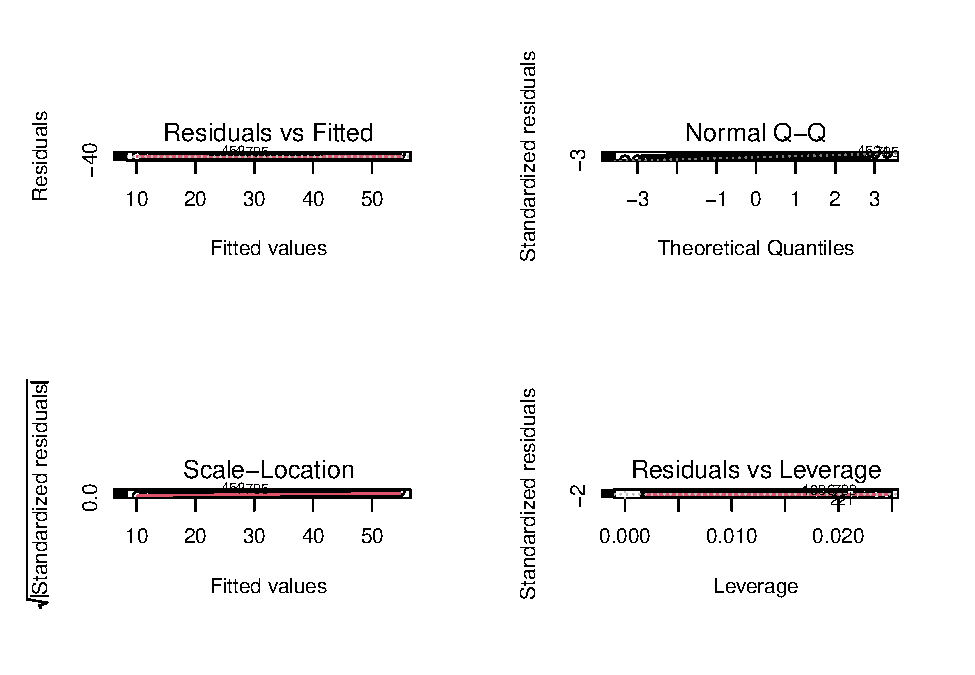
\includegraphics{Nexttry_files/figure-latex/unnamed-chunk-2-30.pdf}

\begin{Shaded}
\begin{Highlighting}[]
\FunctionTok{par}\NormalTok{(}\AttributeTok{mfrow=}\FunctionTok{c}\NormalTok{(}\DecValTok{1}\NormalTok{,}\DecValTok{1}\NormalTok{))}


\CommentTok{\# TABLE 1:}

\CommentTok{\# Model 1: INITIAL MODEL:}
\NormalTok{model1}\OtherTok{\textless{}{-}}\FunctionTok{lm}\NormalTok{(SUIC\_RISK}\SpecialCharTok{\textasciitilde{}}\NormalTok{SEX}\SpecialCharTok{+}\NormalTok{AGE}\SpecialCharTok{+}\NormalTok{PROVINCE}\SpecialCharTok{+}\NormalTok{EDUCATION}\SpecialCharTok{+}\NormalTok{ECONOMIC\_INCOME}\SpecialCharTok{+}\NormalTok{LIVING\_WITH\_SOMEBODY}\SpecialCharTok{+}\NormalTok{MENTAL\_DISORDER\_HISTORY}\SpecialCharTok{+}\NormalTok{SUIC\_ATTEMPT\_HISTORY}\SpecialCharTok{+}\NormalTok{SUB\_PERIODS,}\AttributeTok{data=}\NormalTok{table)}
\FunctionTok{summary}\NormalTok{(model1)}
\end{Highlighting}
\end{Shaded}

\begin{verbatim}
## 
## Call:
## lm(formula = SUIC_RISK ~ SEX + AGE + PROVINCE + EDUCATION + ECONOMIC_INCOME + 
##     LIVING_WITH_SOMEBODY + MENTAL_DISORDER_HISTORY + SUIC_ATTEMPT_HISTORY + 
##     SUB_PERIODS, data = table)
## 
## Residuals:
##     Min      1Q  Median      3Q     Max 
## -37.524  -8.719  -1.462   7.951  48.935 
## 
## Coefficients:
##                                             Estimate Std. Error t value
## (Intercept)                                 27.69881    9.79918   2.827
## SEXwoman                                     2.62687    1.04714   2.509
## AGE                                         -0.22315    0.04107  -5.433
## PROVINCECABA (Buenos Aires capital)         -1.01982    1.63071  -0.625
## PROVINCECatamarca                           18.56827    9.61317   1.932
## PROVINCEChaco                               -8.60127    5.14607  -1.671
## PROVINCEChubut                              -5.92589    6.73562  -0.880
## PROVINCECórdoba                             -4.59394    1.26175  -3.641
## PROVINCECorrientes                          -4.93970    6.04192  -0.818
## PROVINCEEntre Ríos                          -0.87557    3.60142  -0.243
## PROVINCEFormosa                             -2.80126    7.76443  -0.361
## PROVINCEJujuy                               -1.74883    2.48261  -0.704
## PROVINCELa Pampa                            -7.55391    4.82045  -1.567
## PROVINCELa Rioja                           -15.75108   13.40919  -1.175
## PROVINCEMendoza                             -1.75830    3.39769  -0.517
## PROVINCEMisiones                            -8.59913    3.69313  -2.328
## PROVINCENeuquén                             -9.98776    4.67488  -2.136
## PROVINCEother                               -3.63925    3.32741  -1.094
## PROVINCEOtro                                 2.94492    7.84247   0.376
## PROVINCERío Negro                           -1.65830    6.73772  -0.246
## PROVINCESalta                                3.92532    3.97722   0.987
## PROVINCESan Juan                            -1.99197    6.78091  -0.294
## PROVINCESan Luis                            14.21141   13.39591   1.061
## PROVINCESanta Cruz                           6.53366    9.47525   0.690
## PROVINCESanta Fe                            -3.70252    1.25480  -2.951
## PROVINCESantiago del Estero                 -7.20920    3.69485  -1.951
## PROVINCETierra del Fuego                    -1.45036    3.22680  -0.449
## PROVINCETucumán                             -2.88133    2.81793  -1.022
## EDUCATIONCompleted high school              18.31089    9.57557   1.912
## EDUCATIONCompleted postgraduate             17.51758    9.57449   1.830
## EDUCATIONCompleted tertiary or university   16.75244    9.52883   1.758
## EDUCATIONIncomplete elementary school       16.58362   16.36473   1.013
## EDUCATIONIncomplete high school             23.92673    9.88982   2.419
## EDUCATIONIncomplete postgraduate            17.76509    9.61258   1.848
## EDUCATIONIncomplete tertiary or university  18.02646    9.51795   1.894
## EDUCATIONOtro                               13.60416   13.57994   1.002
## ECONOMIC_INCOMEyes                          -2.23014    1.13851  -1.959
## LIVING_WITH_SOMEBODYyes                      0.43347    1.17898   0.368
## MENTAL_DISORDER_HISTORYyes                   6.18680    0.96138   6.435
## SUIC_ATTEMPT_HISTORYno                     -13.11713    0.99285 -13.212
## SUIC_ATTEMPT_HISTORYyes                      5.42338    1.78599   3.037
## SUB_PERIODS2./3. EXT POST                    1.09499    1.18586   0.923
## SUB_PERIODS4. EXT POST                       1.43317    1.09544   1.308
##                                            Pr(>|t|)    
## (Intercept)                                0.004793 ** 
## SEXwoman                                   0.012269 *  
## AGE                                        6.87e-08 ***
## PROVINCECABA (Buenos Aires capital)        0.531854    
## PROVINCECatamarca                          0.053683 .  
## PROVINCEChaco                              0.094934 .  
## PROVINCEChubut                             0.379176    
## PROVINCECórdoba                            0.000285 ***
## PROVINCECorrientes                         0.413786    
## PROVINCEEntre Ríos                         0.807961    
## PROVINCEFormosa                            0.718335    
## PROVINCEJujuy                              0.481320    
## PROVINCELa Pampa                           0.117401    
## PROVINCELa Rioja                           0.240400    
## PROVINCEMendoza                            0.604917    
## PROVINCEMisiones                           0.020078 *  
## PROVINCENeuquén                            0.032870 *  
## PROVINCEother                              0.274327    
## PROVINCEOtro                               0.707357    
## PROVINCERío Negro                          0.805635    
## PROVINCESalta                              0.323893    
## PROVINCESan Juan                           0.768998    
## PROVINCESan Luis                           0.288988    
## PROVINCESanta Cruz                         0.490628    
## PROVINCESanta Fe                           0.003241 ** 
## PROVINCESantiago del Estero                0.051304 .  
## PROVINCETierra del Fuego                   0.653183    
## PROVINCETucumán                            0.306779    
## EDUCATIONCompleted high school             0.056114 .  
## EDUCATIONCompleted postgraduate            0.067590 .  
## EDUCATIONCompleted tertiary or university  0.079023 .  
## EDUCATIONIncomplete elementary school      0.311113    
## EDUCATIONIncomplete high school            0.015717 *  
## EDUCATIONIncomplete postgraduate           0.064866 .  
## EDUCATIONIncomplete tertiary or university 0.058505 .  
## EDUCATIONOtro                              0.316677    
## ECONOMIC_INCOMEyes                         0.050395 .  
## LIVING_WITH_SOMEBODYyes                    0.713195    
## MENTAL_DISORDER_HISTORYyes                 1.86e-10 ***
## SUIC_ATTEMPT_HISTORYno                      < 2e-16 ***
## SUIC_ATTEMPT_HISTORYyes                    0.002451 ** 
## SUB_PERIODS2./3. EXT POST                  0.356022    
## SUB_PERIODS4. EXT POST                     0.191054    
## ---
## Signif. codes:  0 '***' 0.001 '**' 0.01 '*' 0.05 '.' 0.1 ' ' 1
## 
## Residual standard error: 13.28 on 1057 degrees of freedom
## Multiple R-squared:  0.3646, Adjusted R-squared:  0.3394 
## F-statistic: 14.44 on 42 and 1057 DF,  p-value: < 2.2e-16
\end{verbatim}

\begin{Shaded}
\begin{Highlighting}[]
\CommentTok{\# YES significative p{-}value \textless{} 2.2e{-}16}

\CommentTok{\# Model 2 eliminates PROVINCE:}
\NormalTok{model2}\OtherTok{\textless{}{-}}\FunctionTok{lm}\NormalTok{(SUIC\_RISK}\SpecialCharTok{\textasciitilde{}}\NormalTok{SEX}\SpecialCharTok{+}\NormalTok{AGE}\SpecialCharTok{+}\NormalTok{EDUCATION}\SpecialCharTok{+}\NormalTok{ECONOMIC\_INCOME}\SpecialCharTok{+}\NormalTok{LIVING\_WITH\_SOMEBODY}\SpecialCharTok{+}\NormalTok{MENTAL\_DISORDER\_HISTORY}\SpecialCharTok{+}\NormalTok{SUIC\_ATTEMPT\_HISTORY}\SpecialCharTok{+}\NormalTok{SUB\_PERIODS,}\AttributeTok{data=}\NormalTok{table)}
\FunctionTok{summary}\NormalTok{(model2)}
\end{Highlighting}
\end{Shaded}

\begin{verbatim}
## 
## Call:
## lm(formula = SUIC_RISK ~ SEX + AGE + EDUCATION + ECONOMIC_INCOME + 
##     LIVING_WITH_SOMEBODY + MENTAL_DISORDER_HISTORY + SUIC_ATTEMPT_HISTORY + 
##     SUB_PERIODS, data = table)
## 
## Residuals:
##     Min      1Q  Median      3Q     Max 
## -38.662  -9.189  -1.186   8.118  48.703 
## 
## Coefficients:
##                                             Estimate Std. Error t value
## (Intercept)                                 26.36871    9.83349   2.682
## SEXwoman                                     2.63105    1.03621   2.539
## AGE                                         -0.23116    0.04029  -5.737
## EDUCATIONCompleted high school              17.56089    9.62349   1.825
## EDUCATIONCompleted postgraduate             16.67919    9.60635   1.736
## EDUCATIONCompleted tertiary or university   16.26577    9.57614   1.699
## EDUCATIONIncomplete elementary school       15.26265   16.45836   0.927
## EDUCATIONIncomplete high school             24.09927    9.92141   2.429
## EDUCATIONIncomplete postgraduate            17.21498    9.65483   1.783
## EDUCATIONIncomplete tertiary or university  17.40333    9.56648   1.819
## EDUCATIONOtro                                8.59065   13.42457   0.640
## ECONOMIC_INCOMEyes                          -2.36151    1.13706  -2.077
## LIVING_WITH_SOMEBODYyes                     -0.05339    1.16846  -0.046
## MENTAL_DISORDER_HISTORYyes                   6.33147    0.95826   6.607
## SUIC_ATTEMPT_HISTORYno                     -13.39501    0.98652 -13.578
## SUIC_ATTEMPT_HISTORYyes                      5.10064    1.78434   2.859
## SUB_PERIODS2./3. EXT POST                    1.56311    1.12071   1.395
## SUB_PERIODS4. EXT POST                       1.44676    0.96134   1.505
##                                            Pr(>|t|)    
## (Intercept)                                 0.00744 ** 
## SEXwoman                                    0.01125 *  
## AGE                                        1.25e-08 ***
## EDUCATIONCompleted high school              0.06831 .  
## EDUCATIONCompleted postgraduate             0.08280 .  
## EDUCATIONCompleted tertiary or university   0.08969 .  
## EDUCATIONIncomplete elementary school       0.35395    
## EDUCATIONIncomplete high school             0.01530 *  
## EDUCATIONIncomplete postgraduate            0.07486 .  
## EDUCATIONIncomplete tertiary or university  0.06916 .  
## EDUCATIONOtro                               0.52236    
## ECONOMIC_INCOMEyes                          0.03805 *  
## LIVING_WITH_SOMEBODYyes                     0.96356    
## MENTAL_DISORDER_HISTORYyes                 6.13e-11 ***
## SUIC_ATTEMPT_HISTORYno                      < 2e-16 ***
## SUIC_ATTEMPT_HISTORYyes                     0.00434 ** 
## SUB_PERIODS2./3. EXT POST                   0.16338    
## SUB_PERIODS4. EXT POST                      0.13263    
## ---
## Signif. codes:  0 '***' 0.001 '**' 0.01 '*' 0.05 '.' 0.1 ' ' 1
## 
## Residual standard error: 13.37 on 1082 degrees of freedom
## Multiple R-squared:  0.3407, Adjusted R-squared:  0.3303 
## F-statistic: 32.89 on 17 and 1082 DF,  p-value: < 2.2e-16
\end{verbatim}

\begin{Shaded}
\begin{Highlighting}[]
\CommentTok{\# YES significative p{-}value \textless{} 2.2e{-}16}

\CommentTok{\# Model 3 eliminates EDUCATION:}
\NormalTok{model3}\OtherTok{\textless{}{-}}\FunctionTok{lm}\NormalTok{(SUIC\_RISK}\SpecialCharTok{\textasciitilde{}}\NormalTok{SEX}\SpecialCharTok{+}\NormalTok{AGE}\SpecialCharTok{+}\NormalTok{ECONOMIC\_INCOME}\SpecialCharTok{+}\NormalTok{LIVING\_WITH\_SOMEBODY}\SpecialCharTok{+}\NormalTok{MENTAL\_DISORDER\_HISTORY}\SpecialCharTok{+}\NormalTok{SUIC\_ATTEMPT\_HISTORY}\SpecialCharTok{+}\NormalTok{SUB\_PERIODS,}\AttributeTok{data=}\NormalTok{table)}
\FunctionTok{summary}\NormalTok{(model3)}
\end{Highlighting}
\end{Shaded}

\begin{verbatim}
## 
## Call:
## lm(formula = SUIC_RISK ~ SEX + AGE + ECONOMIC_INCOME + LIVING_WITH_SOMEBODY + 
##     MENTAL_DISORDER_HISTORY + SUIC_ATTEMPT_HISTORY + SUB_PERIODS, 
##     data = table)
## 
## Residuals:
##     Min      1Q  Median      3Q     Max 
## -38.503  -9.177  -1.378   7.997  49.044 
## 
## Coefficients:
##                             Estimate Std. Error t value Pr(>|t|)    
## (Intercept)                 44.37273    2.26294  19.608  < 2e-16 ***
## SEXwoman                     2.56109    1.03272   2.480  0.01329 *  
## AGE                         -0.24446    0.03739  -6.538 9.59e-11 ***
## ECONOMIC_INCOMEyes          -2.69348    1.11685  -2.412  0.01604 *  
## LIVING_WITH_SOMEBODYyes     -0.10990    1.16155  -0.095  0.92464    
## MENTAL_DISORDER_HISTORYyes   6.14246    0.95587   6.426 1.95e-10 ***
## SUIC_ATTEMPT_HISTORYno     -13.48316    0.97791 -13.788  < 2e-16 ***
## SUIC_ATTEMPT_HISTORYyes      5.48495    1.78068   3.080  0.00212 ** 
## SUB_PERIODS2./3. EXT POST    1.61984    1.12007   1.446  0.14841    
## SUB_PERIODS4. EXT POST       1.42552    0.95417   1.494  0.13547    
## ---
## Signif. codes:  0 '***' 0.001 '**' 0.01 '*' 0.05 '.' 0.1 ' ' 1
## 
## Residual standard error: 13.39 on 1090 degrees of freedom
## Multiple R-squared:  0.3336, Adjusted R-squared:  0.3281 
## F-statistic: 60.64 on 9 and 1090 DF,  p-value: < 2.2e-16
\end{verbatim}

\begin{Shaded}
\begin{Highlighting}[]
\CommentTok{\# YES significative p{-}value \textless{} 2.2e{-}16}

\CommentTok{\# Model 4 eliminates LIVING\_WITH\_SOMEBODY:}
\NormalTok{model4}\OtherTok{\textless{}{-}}\FunctionTok{lm}\NormalTok{(SUIC\_RISK}\SpecialCharTok{\textasciitilde{}}\NormalTok{SEX}\SpecialCharTok{+}\NormalTok{AGE}\SpecialCharTok{+}\NormalTok{ECONOMIC\_INCOME}\SpecialCharTok{+}\NormalTok{MENTAL\_DISORDER\_HISTORY}\SpecialCharTok{+}\NormalTok{SUIC\_ATTEMPT\_HISTORY}\SpecialCharTok{+}\NormalTok{SUB\_PERIODS,}\AttributeTok{data=}\NormalTok{table)}
\FunctionTok{summary}\NormalTok{(model4)}
\end{Highlighting}
\end{Shaded}

\begin{verbatim}
## 
## Call:
## lm(formula = SUIC_RISK ~ SEX + AGE + ECONOMIC_INCOME + MENTAL_DISORDER_HISTORY + 
##     SUIC_ATTEMPT_HISTORY + SUB_PERIODS, data = table)
## 
## Residuals:
##     Min      1Q  Median      3Q     Max 
## -38.512  -9.188  -1.389   7.984  49.033 
## 
## Coefficients:
##                             Estimate Std. Error t value Pr(>|t|)    
## (Intercept)                 44.26331    1.94422  22.767  < 2e-16 ***
## SEXwoman                     2.55438    1.02981   2.480  0.01327 *  
## AGE                         -0.24398    0.03703  -6.589 6.87e-11 ***
## ECONOMIC_INCOMEyes          -2.68690    1.11418  -2.412  0.01605 *  
## MENTAL_DISORDER_HISTORYyes   6.14858    0.95325   6.450 1.68e-10 ***
## SUIC_ATTEMPT_HISTORYno     -13.48378    0.97744 -13.795  < 2e-16 ***
## SUIC_ATTEMPT_HISTORYyes      5.49220    1.77822   3.089  0.00206 ** 
## SUB_PERIODS2./3. EXT POST    1.61540    1.11858   1.444  0.14898    
## SUB_PERIODS4. EXT POST       1.42500    0.95372   1.494  0.13543    
## ---
## Signif. codes:  0 '***' 0.001 '**' 0.01 '*' 0.05 '.' 0.1 ' ' 1
## 
## Residual standard error: 13.39 on 1091 degrees of freedom
## Multiple R-squared:  0.3336, Adjusted R-squared:  0.3287 
## F-statistic: 68.28 on 8 and 1091 DF,  p-value: < 2.2e-16
\end{verbatim}

\begin{Shaded}
\begin{Highlighting}[]
\CommentTok{\# YES significative p{-}value \textless{} 2.2e{-}16}

\CommentTok{\# Model 5 eliminates SUB PERIODS:}
\NormalTok{model5}\OtherTok{\textless{}{-}}\FunctionTok{lm}\NormalTok{(SUIC\_RISK}\SpecialCharTok{\textasciitilde{}}\NormalTok{SEX}\SpecialCharTok{+}\NormalTok{AGE}\SpecialCharTok{+}\NormalTok{ECONOMIC\_INCOME}\SpecialCharTok{+}\NormalTok{MENTAL\_DISORDER\_HISTORY}\SpecialCharTok{+}\NormalTok{SUIC\_ATTEMPT\_HISTORY,}\AttributeTok{data=}\NormalTok{table)}
\FunctionTok{summary}\NormalTok{(model5)}
\end{Highlighting}
\end{Shaded}

\begin{verbatim}
## 
## Call:
## lm(formula = SUIC_RISK ~ SEX + AGE + ECONOMIC_INCOME + MENTAL_DISORDER_HISTORY + 
##     SUIC_ATTEMPT_HISTORY, data = table)
## 
## Residuals:
##     Min      1Q  Median      3Q     Max 
## -38.172  -9.329  -1.317   7.985  49.689 
## 
## Coefficients:
##                             Estimate Std. Error t value Pr(>|t|)    
## (Intercept)                 45.57130    1.74704  26.085  < 2e-16 ***
## SEXwoman                     2.50060    1.02370   2.443   0.0147 *  
## AGE                         -0.25374    0.03578  -7.091 2.38e-12 ***
## ECONOMIC_INCOMEyes          -2.65920    1.11441  -2.386   0.0172 *  
## MENTAL_DISORDER_HISTORYyes   6.17526    0.95324   6.478 1.40e-10 ***
## SUIC_ATTEMPT_HISTORYno     -13.47415    0.97731 -13.787  < 2e-16 ***
## SUIC_ATTEMPT_HISTORYyes      5.53602    1.77790   3.114   0.0019 ** 
## ---
## Signif. codes:  0 '***' 0.001 '**' 0.01 '*' 0.05 '.' 0.1 ' ' 1
## 
## Residual standard error: 13.39 on 1093 degrees of freedom
## Multiple R-squared:  0.3318, Adjusted R-squared:  0.3282 
## F-statistic: 90.47 on 6 and 1093 DF,  p-value: < 2.2e-16
\end{verbatim}

\begin{Shaded}
\begin{Highlighting}[]
\CommentTok{\# YES significative p{-}value \textless{} 2.2e{-}16}


\DocumentationTok{\#\#\#\#\#\#\#\#\#\#\#\#\#\#\#\#}
\DocumentationTok{\#\# Considering the predictors included in the best{-}fitted model (i.e., stepwith) in this group, we analyzed the smallest possible linear model for each specific MHS indicator by means of all two{-}predictor combinations.  }
\CommentTok{\# We performed all{-}subsets regression using the regsubsets() function from the leaps package.}
\CommentTok{\# We analyzed the three best models for two{-}predictor subset sizes.}

\NormalTok{leapsbestwith}\OtherTok{\textless{}{-}}\FunctionTok{regsubsets}\NormalTok{(SUIC\_RISK}\SpecialCharTok{\textasciitilde{}}\NormalTok{SEX}\SpecialCharTok{+}\NormalTok{AGE}\SpecialCharTok{+}\NormalTok{ECONOMIC\_INCOME}\SpecialCharTok{+}\NormalTok{MENTAL\_DISORDER\_HISTORY}\SpecialCharTok{+}\NormalTok{SUIC\_ATTEMPT\_HISTORY,}\AttributeTok{data=}\NormalTok{table,}\AttributeTok{nbest=}\DecValTok{3}\NormalTok{)}
\FunctionTok{summary}\NormalTok{(leapsbestwith)}
\end{Highlighting}
\end{Shaded}

\begin{verbatim}
## Subset selection object
## Call: regsubsets.formula(SUIC_RISK ~ SEX + AGE + ECONOMIC_INCOME + 
##     MENTAL_DISORDER_HISTORY + SUIC_ATTEMPT_HISTORY, data = table, 
##     nbest = 3)
## 6 Variables  (and intercept)
##                            Forced in Forced out
## SEXwoman                       FALSE      FALSE
## AGE                            FALSE      FALSE
## ECONOMIC_INCOMEyes             FALSE      FALSE
## MENTAL_DISORDER_HISTORYyes     FALSE      FALSE
## SUIC_ATTEMPT_HISTORYno         FALSE      FALSE
## SUIC_ATTEMPT_HISTORYyes        FALSE      FALSE
## 3 subsets of each size up to 6
## Selection Algorithm: exhaustive
##          SEXwoman AGE ECONOMIC_INCOMEyes MENTAL_DISORDER_HISTORYyes
## 1  ( 1 ) " "      " " " "                " "                       
## 1  ( 2 ) " "      " " " "                " "                       
## 1  ( 3 ) " "      " " " "                "*"                       
## 2  ( 1 ) " "      "*" " "                " "                       
## 2  ( 2 ) " "      " " " "                "*"                       
## 2  ( 3 ) " "      " " "*"                " "                       
## 3  ( 1 ) " "      "*" " "                "*"                       
## 3  ( 2 ) " "      "*" " "                " "                       
## 3  ( 3 ) " "      "*" "*"                " "                       
## 4  ( 1 ) " "      "*" " "                "*"                       
## 4  ( 2 ) "*"      "*" " "                "*"                       
## 4  ( 3 ) " "      "*" "*"                "*"                       
## 5  ( 1 ) "*"      "*" " "                "*"                       
## 5  ( 2 ) " "      "*" "*"                "*"                       
## 5  ( 3 ) "*"      "*" "*"                "*"                       
## 6  ( 1 ) "*"      "*" "*"                "*"                       
##          SUIC_ATTEMPT_HISTORYno SUIC_ATTEMPT_HISTORYyes
## 1  ( 1 ) "*"                    " "                    
## 1  ( 2 ) " "                    "*"                    
## 1  ( 3 ) " "                    " "                    
## 2  ( 1 ) "*"                    " "                    
## 2  ( 2 ) "*"                    " "                    
## 2  ( 3 ) "*"                    " "                    
## 3  ( 1 ) "*"                    " "                    
## 3  ( 2 ) "*"                    "*"                    
## 3  ( 3 ) "*"                    " "                    
## 4  ( 1 ) "*"                    "*"                    
## 4  ( 2 ) "*"                    " "                    
## 4  ( 3 ) "*"                    " "                    
## 5  ( 1 ) "*"                    "*"                    
## 5  ( 2 ) "*"                    "*"                    
## 5  ( 3 ) "*"                    " "                    
## 6  ( 1 ) "*"                    "*"
\end{verbatim}

\begin{Shaded}
\begin{Highlighting}[]
\CommentTok{\# The best two{-}predictors model was: ANXIETY\_STATE \textasciitilde{} AGE + SUIC\_ATTEMPT\_HISTORY==no}

\FunctionTok{plot}\NormalTok{(leapsbestwith,}\AttributeTok{scale=}\StringTok{"r2"}\NormalTok{)}
\end{Highlighting}
\end{Shaded}

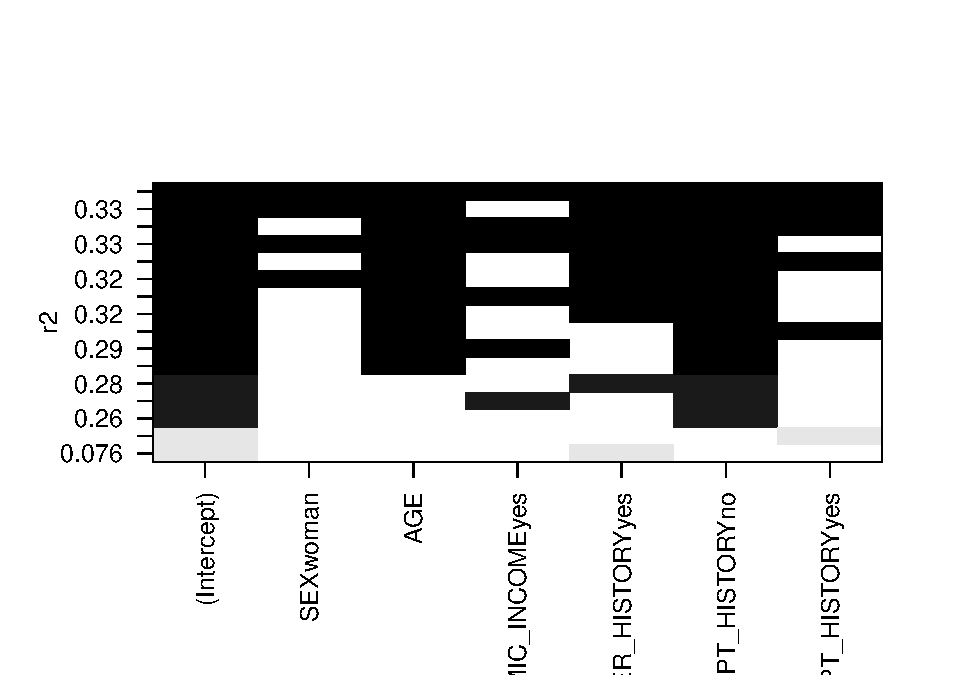
\includegraphics{Nexttry_files/figure-latex/unnamed-chunk-2-31.pdf}

\begin{Shaded}
\begin{Highlighting}[]
\FunctionTok{plot}\NormalTok{(leapsbestwith,}\AttributeTok{scale=}\StringTok{"adjr2"}\NormalTok{)}
\end{Highlighting}
\end{Shaded}

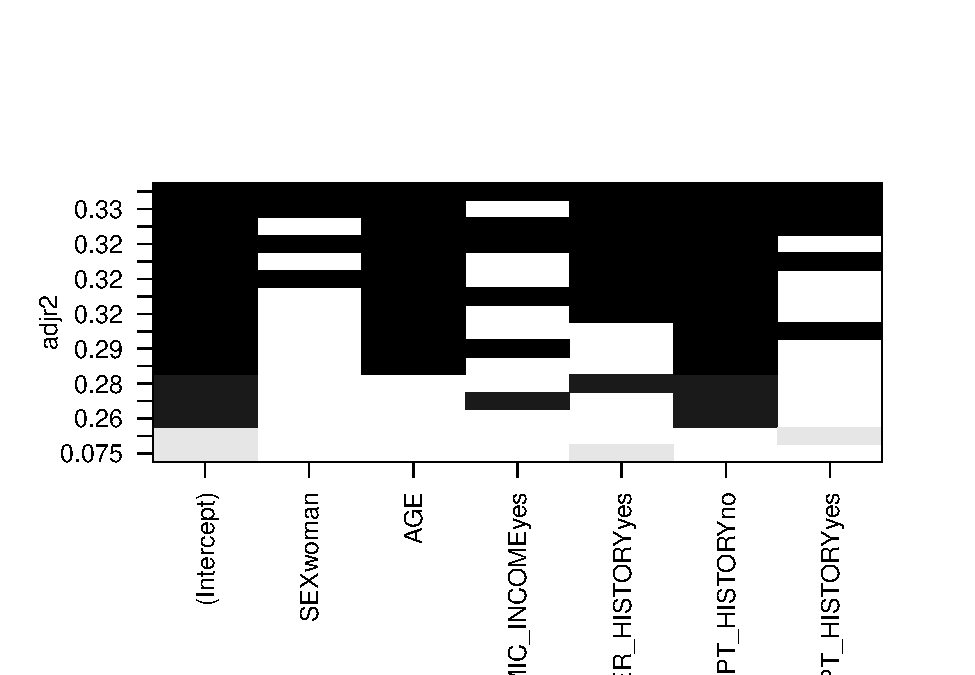
\includegraphics{Nexttry_files/figure-latex/unnamed-chunk-2-32.pdf}

\begin{Shaded}
\begin{Highlighting}[]
\CommentTok{\# First: AGE + SUIC\_ATTEMPT\_HISTORY (no):}
\NormalTok{besttwowithfirst}\OtherTok{\textless{}{-}}\FunctionTok{lm}\NormalTok{(SUIC\_RISK}\SpecialCharTok{\textasciitilde{}}\NormalTok{AGE}\SpecialCharTok{+}\NormalTok{SUIC\_ATTEMPT\_HISTORY,}\AttributeTok{data=}\NormalTok{table)}
\NormalTok{besttwowithfirst}
\end{Highlighting}
\end{Shaded}

\begin{verbatim}
## 
## Call:
## lm(formula = SUIC_RISK ~ AGE + SUIC_ATTEMPT_HISTORY, data = table)
## 
## Coefficients:
##             (Intercept)                      AGE   SUIC_ATTEMPT_HISTORYno  
##                 47.7289                  -0.2443                 -15.1119  
## SUIC_ATTEMPT_HISTORYyes  
##                  6.9983
\end{verbatim}

\begin{Shaded}
\begin{Highlighting}[]
\FunctionTok{summary}\NormalTok{(besttwowithfirst)}
\end{Highlighting}
\end{Shaded}

\begin{verbatim}
## 
## Call:
## lm(formula = SUIC_RISK ~ AGE + SUIC_ATTEMPT_HISTORY, data = table)
## 
## Residuals:
##     Min      1Q  Median      3Q     Max 
## -34.555  -9.596  -1.588   8.025  48.781 
## 
## Coefficients:
##                          Estimate Std. Error t value Pr(>|t|)    
## (Intercept)              47.72894    1.27892  37.320  < 2e-16 ***
## AGE                      -0.24434    0.03588  -6.810 1.61e-11 ***
## SUIC_ATTEMPT_HISTORYno  -15.11187    0.97372 -15.520  < 2e-16 ***
## SUIC_ATTEMPT_HISTORYyes   6.99832    1.80927   3.868 0.000116 ***
## ---
## Signif. codes:  0 '***' 0.001 '**' 0.01 '*' 0.05 '.' 0.1 ' ' 1
## 
## Residual standard error: 13.71 on 1096 degrees of freedom
## Multiple R-squared:  0.2976, Adjusted R-squared:  0.2957 
## F-statistic: 154.8 on 3 and 1096 DF,  p-value: < 2.2e-16
\end{verbatim}

\begin{Shaded}
\begin{Highlighting}[]
\FunctionTok{confint}\NormalTok{(besttwowithfirst)}
\end{Highlighting}
\end{Shaded}

\begin{verbatim}
##                               2.5 %      97.5 %
## (Intercept)              45.2195375  50.2383518
## AGE                      -0.3147459  -0.1739428
## SUIC_ATTEMPT_HISTORYno  -17.0224394 -13.2012929
## SUIC_ATTEMPT_HISTORYyes   3.4482992  10.5483376
\end{verbatim}

\begin{Shaded}
\begin{Highlighting}[]
\CommentTok{\# Second: MENTAL DISORDER (yes) + SUIC\_ATTEMPT\_HISTORY (no):}
\NormalTok{besttwowithsecond}\OtherTok{\textless{}{-}}\FunctionTok{lm}\NormalTok{(SUIC\_RISK}\SpecialCharTok{\textasciitilde{}}\NormalTok{MENTAL\_DISORDER\_HISTORY}\SpecialCharTok{+}\NormalTok{SUIC\_ATTEMPT\_HISTORY,}\AttributeTok{data=}\NormalTok{table)}
\NormalTok{besttwowithsecond}
\end{Highlighting}
\end{Shaded}

\begin{verbatim}
## 
## Call:
## lm(formula = SUIC_RISK ~ MENTAL_DISORDER_HISTORY + SUIC_ATTEMPT_HISTORY, 
##     data = table)
## 
## Coefficients:
##                (Intercept)  MENTAL_DISORDER_HISTORYyes  
##                     38.833                       5.468  
##     SUIC_ATTEMPT_HISTORYno     SUIC_ATTEMPT_HISTORYyes  
##                    -15.353                       5.422
\end{verbatim}

\begin{Shaded}
\begin{Highlighting}[]
\FunctionTok{summary}\NormalTok{(besttwowithsecond)}
\end{Highlighting}
\end{Shaded}

\begin{verbatim}
## 
## Call:
## lm(formula = SUIC_RISK ~ MENTAL_DISORDER_HISTORY + SUIC_ATTEMPT_HISTORY, 
##     data = table)
## 
## Residuals:
##    Min     1Q Median     3Q    Max 
## -40.30  -9.48  -1.48   7.52  49.52 
## 
## Coefficients:
##                            Estimate Std. Error t value Pr(>|t|)    
## (Intercept)                 38.8331     0.9006  43.121  < 2e-16 ***
## MENTAL_DISORDER_HISTORYyes   5.4681     0.9741   5.613 2.51e-08 ***
## SUIC_ATTEMPT_HISTORYno     -15.3533     0.9797 -15.672  < 2e-16 ***
## SUIC_ATTEMPT_HISTORYyes      5.4216     1.8288   2.965   0.0031 ** 
## ---
## Signif. codes:  0 '***' 0.001 '**' 0.01 '*' 0.05 '.' 0.1 ' ' 1
## 
## Residual standard error: 13.8 on 1096 degrees of freedom
## Multiple R-squared:  0.2884, Adjusted R-squared:  0.2864 
## F-statistic: 148.1 on 3 and 1096 DF,  p-value: < 2.2e-16
\end{verbatim}

\begin{Shaded}
\begin{Highlighting}[]
\FunctionTok{confint}\NormalTok{(besttwowithsecond)}
\end{Highlighting}
\end{Shaded}

\begin{verbatim}
##                                 2.5 %     97.5 %
## (Intercept)                 37.066113  40.600112
## MENTAL_DISORDER_HISTORYyes   3.556768   7.379458
## SUIC_ATTEMPT_HISTORYno     -17.275587 -13.431048
## SUIC_ATTEMPT_HISTORYyes      1.833339   9.009860
\end{verbatim}

\begin{Shaded}
\begin{Highlighting}[]
\CommentTok{\# Third: ECONOMIC\_INCOME (yes) + SUIC\_ATTEMPT\_HISTORY (no):}
\NormalTok{besttwowiththird}\OtherTok{\textless{}{-}}\FunctionTok{lm}\NormalTok{(SUIC\_RISK}\SpecialCharTok{\textasciitilde{}}\NormalTok{ECONOMIC\_INCOME}\SpecialCharTok{+}\NormalTok{SUIC\_ATTEMPT\_HISTORY,}\AttributeTok{data=}\NormalTok{table)}
\NormalTok{besttwowiththird}
\end{Highlighting}
\end{Shaded}

\begin{verbatim}
## 
## Call:
## lm(formula = SUIC_RISK ~ ECONOMIC_INCOME + SUIC_ATTEMPT_HISTORY, 
##     data = table)
## 
## Coefficients:
##             (Intercept)       ECONOMIC_INCOMEyes   SUIC_ATTEMPT_HISTORYno  
##                  44.233                   -4.034                  -16.237  
## SUIC_ATTEMPT_HISTORYyes  
##                   6.237
\end{verbatim}

\begin{Shaded}
\begin{Highlighting}[]
\FunctionTok{summary}\NormalTok{(besttwowiththird)}
\end{Highlighting}
\end{Shaded}

\begin{verbatim}
## 
## Call:
## lm(formula = SUIC_RISK ~ ECONOMIC_INCOME + SUIC_ATTEMPT_HISTORY, 
##     data = table)
## 
## Residuals:
##     Min      1Q  Median      3Q     Max 
## -40.436  -9.962  -1.962   7.801  53.038 
## 
## Coefficients:
##                         Estimate Std. Error t value Pr(>|t|)    
## (Intercept)               44.233      1.234  35.832  < 2e-16 ***
## ECONOMIC_INCOMEyes        -4.034      1.145  -3.525 0.000442 ***
## SUIC_ATTEMPT_HISTORYno   -16.238      0.970 -16.740  < 2e-16 ***
## SUIC_ATTEMPT_HISTORYyes    6.237      1.836   3.397 0.000706 ***
## ---
## Signif. codes:  0 '***' 0.001 '**' 0.01 '*' 0.05 '.' 0.1 ' ' 1
## 
## Residual standard error: 13.92 on 1096 degrees of freedom
## Multiple R-squared:  0.2761, Adjusted R-squared:  0.2742 
## F-statistic: 139.4 on 3 and 1096 DF,  p-value: < 2.2e-16
\end{verbatim}

\begin{Shaded}
\begin{Highlighting}[]
\FunctionTok{confint}\NormalTok{(besttwowiththird)}
\end{Highlighting}
\end{Shaded}

\begin{verbatim}
##                              2.5 %     97.5 %
## (Intercept)              41.810619  46.654886
## ECONOMIC_INCOMEyes       -6.279346  -1.788186
## SUIC_ATTEMPT_HISTORYno  -18.140646 -14.334281
## SUIC_ATTEMPT_HISTORYyes   2.634389   9.839644
\end{verbatim}

```

  \bibliography{book.bib,packages.bib,referenties.bib}

\end{document}
